% Fichero principal para libro de MATLAB y Octave para editorial Garceta
\documentclass[11pt, table]{book}

% -----------------------------------------------
% Título y autor
% -----------------------------------------------
\title{Introducción a la programación funcional}
\author{Santiago Higuera de Frutos \\ \vspace{1em}\small Universidad Politécnica de Madrid}
\date{ 
	\begin{center}
		\includegraphics[width=0.3\textwidth]{img/Rustacean-orig-noshadow.png}
	\end{center}
%	\begin{center}
%		\includegraphics[width=0.25\textwidth]{img/rust-logo.png}
%	\end{center}
   \begin{center}
      \footnotesize \textbf{\color{red}(Versión de fecha  \today)}
   \end{center}
}

% Fichero de estilo para este libro
\usepackage{../../garceta_2024}
\usepackage{../../codeboxes}



% -----------------------------------------------
% Inicio del documento
% -----------------------------------------------
\begin{document}
\lstset{language=Rust, style=colouredRust}

\pagestyle{empty}

\begin{center}
   \includegraphics[width=\textwidth]{img/banner_ice.png}
\end{center}

{\centering \vspace{5em} \Huge\bfseries  Introducción a la programación funcional \par}

{\vspace{2em} \centering Santiago Higuera de Frutos \par}

{\centering \small Universidad Politécnica de Madrid \par}

\begin{center}
   \includegraphics[width=0.3\textwidth]{img/Rustacean-orig-noshadow.png}
\end{center}
%	\begin{center}
   %		\includegraphics[width=0.25\textwidth]{img/rust-logo.png}
   %	\end{center}
\begin{center}
   \footnotesize \textbf{\color{red}(Versión de fecha  \today)}
\end{center}


%\maketitle


\blankpage
%\pagestyle{fancy}
% -----------------------------------
% Dedicatoria
\pagestyle{empty}

\vfill
\begin{flushright}
\begin{minipage}{0.7\textwidth}
\begin{flushright}
\footnotesize
\textit{A los alumnos y profesores de la Universidad Politécnica de Madrid y al oficio de profesor, que tan pocos reconocimientos recibe, a pesar de su importancia en la creación de una sociedad mejor.} \\
\textbf{Santiago}
\end{flushright}
\end{minipage}
\end{flushright}

\blankpage


% -----------------------------------
% Tablas de contenidos
\dominitoc
\setcounter{tocdepth}{1} % Índice con secciones
\pagestyle{indice}
\renewcommand{\thepage}{\roman{page}}
\setcounter{page}{7}
{\small
	\tableofcontents
}
\vfill\null
\pagebreak

\blankpage
% ------------------------------------
% Prólogo
% ------------------------------------
\pagestyle{empty}
\chapter*{Prólogo}
\addstarredchapter{Prólogo}
\chaptermark{Prólogo}
\label{sec_prologo}

\noindent La programación funcional no es nueva. El lenguaje LISP (LISt Processing) está considerado uno de los primeros lenguajes de alto nivel que se desarrollaron, junto a Fortran y Cobol. Durante mucho tiempo se ha considerado un paradigma de programación demasiado teórico y alejado de la resolución de los problemas habituales en la programación real.

\smallskip

Durante ese tiempo, la Programación Orientada a Objetos (POO) se consideraba el paradigma base necesario para la programación en cualquier lenguaje. Con el tiempo, la POO ha mostrado algunas de sus debilidades, originadas por el mecanismo de la herencia entre tipos. Ya en 1994 ``\textit{The gang of four}'', en su famoso libro ``\textit{Design Patterns: Elements of Reusable Object-Oriented Software}'',  indicaban que había que primar la composición frente a la herencia al construir los programas \citep{gammaDesignPatternsElements1994}. 

\smallskip

En los últimos años, la programación funcional ha adquirido especial relevancia. Los principios que rigen la programación funcional son muy simples. Los principales lenguajes han ido incorporando algunos de los elementos que caracterizan a la programación funcional, como las funciones de orden superior, las closures, la inmutabilidad y otros. Es posible escribir programas con un estilo funcional casi en cualquier lenguaje.

\smallskip

Rust es un lenguaje de programación con solo unos años de vida pero que está teniendo un crecimiento muy importante debido la seguridad del manejo de memoria que proporciona, a la velocidad de ejecución del código generado, a la calidad de las herramientas que proporciona y a las buenas sensaciones que proporciona al programar. Rust no es un lenguaje funcional estricto, pero proporciona suficientes elementos para poder ser utilizado como tal. 

\smallskip

A lo largo del curso, se va a hacer una introducción a la utilización del lenguaje Rust y a los conceptos que sustentan el paradigma de la programación funcional. Se utilizará principalmente el lenguaje Rust, aunque también se mostrarán ejemplos en otros lenguajes.

\smallskip

Al final del curso, el alumno comprenderá los conceptos que subyacen bajo el paradigma de la programación funcional, de forma que podrá utilizar algunos de ellos en el lenguaje que utilice habitualmente. Ademas, conocerá los conceptos fundamentales de la programación con Rust, lo que le permitirá adentrarse en el lenguaje, si lo considera de interés.

%\blankpage

%\chapter*{Nota}
\addstarredchapter{Nota}
\chaptermark{Nota}
\label{sec_prologo}

\noindent Con el fin de optimizar el tiempo disponible, sería deseable que los alumnos instalaran en los ordenadores que vayan a utilizar en el curso, el entorno de desarrollo de Rust.

\smallskip

El entorno de desarrollo consta del lenguaje Rust y de un editor de texto.

\smallskip

Se adjunta el capítulo 2 de la documentación del curso, en el cual se explica cómo hacerlo.


%\blankpage


\vfill\null
\pagebreak

% -----------------------------------
% Acerca de los autores
\thispagestyle{vacio}
{\centering \huge\textbf{Acerca del autor}\par}
\vspace{6em}

\begin{minipage}{0.9\textwidth}
	\setlength{\parindent}{0pt}
	
	{\centering\large\textbf{Santiago Higuera de Frutos} \par}
	\vspace{1em}
	
	\begin{wrapfigure}{l}{0.4\textwidth} 
		\centering\vspace{-0.5\baselineskip}
		\includegraphics[width=0.4\textwidth]{img/FotoSantiago_bw.jpg}
	\end{wrapfigure}
	
	Doctor Ingeniero de Caminos por la Universidad Politécnica de Madrid (UPM). Ha sido profesor en la Escuela de Ingenieros de Caminos y actualmente en Teleco Campus Sur. Es autor de los libros ``\textit{Programacion en Rust}'' y  ``Programación y métodos numéricos para Ingeniería con MATLAB y Octave'', publicados por la Editorial Garceta, así como de numerosos artículos y conferencias sobre programación, geometría de las carreteras y simuladores de conducción, todo ello en el ámbito del software de código abierto. 
\end{minipage}

\blankpage

\cftpagenumbersoff{section} % Suprime los números de página en las minitablas de contenido generadas con el paquete minitoc. Debido a las interacciones entre tocloft y minitoc, hay que hacerlo desde aquí y no funciona la orden de minitoc \mtcsetpagenumbers{minitoc}{off}. Además, hay que dar la orden después de haber generado el \tableofcontents

\setcounter{minitocdepth}{1} % Índices de los capítulos solo con secciones
% ------------------------------------

% ------------------------------------
% Capítulos
% ------------------------------------
\pagestyle{fancy}
\renewcommand{\thepage}{\arabic{page}}
\setcounter{page}{1}

% Contenido del CursoICE_2024
\chapter{Pensar de manera funcional. Programación declarativa}
\label{ch_intro}

\IndiceCapitulo
\begin{Resumen}
   Se considera que la programación funcional está basada en el \textit{cálculo lambda},  un sistema formal desarrollado en los años 1930 para investigar la naturaleza de las funciones, de la computabilidad y su relación con la recursión. 
   
   \smallskip
   
   El objetivo de este curso es explicar las técnicas y la forma funcional de razonar en programación para mejorar la calidad del código de los programas.
\end{Resumen}

\section{Adiós a la Programación Orientada a Objetos}
\label{sec_adios_poo}
\noindent A partir de los años 90 del siglo pasado, la Programación Orientada a Objetos (POO) se convirtió en el paradigma fundamental de programación. Si no sabías programar orientado a objetos, no sabías programar. Se enseñaba de una forma muy dogmática e incluso se suponía que había que \textit{pensar orientado a objetos}. Cualquier programa se tenía que razonar en términos de clases y objetos, en lo que se denominaba \textit{análisis y diseño orientado a objetos}.

A medida que se fueron desarrollando programas con esta metodología, se comprobó que la POO daba lugar a ciertos desarrollos que producían programas con código complicado, difícil de comprender y que además dificultaba la depuración y la realización de test. Se comprobó que la POO se adaptaba mejor a cierto tipo de problemas que a otros.

El tipo de datos en el que se basa la POO es la \textit{clase}. A las instancias que se crean de una clase determinada se le llaman \textit{objetos}. Las clases incluyen en una misma construcción de programación los datos, frecuentemente llamados \textit{propiedades} y las funciones que operan sobre dichos datos, que se suelen llamar \textit{métodos}. El valor de las propiedades representa el \textit{estado} del objeto; los métodos de la clase representan el \textit{comportamiento} del objeto y proporcionan la forma de modificar su estado.
   
La POO se fundamenta en tres pilares fundamentales: \textit{herencia}, \textit{encapsulación} y  \textit{polimorfismo}.

\vspace{0.7em}
\begin{figure}[htb]
   \begin{center}
      \includegraphics[width=0.4\textwidth]{img/pilares_1.png}
      \caption{Pilares en los que se fundamenta la Programación Orientada a Objetos}
      \label{fig_pilares_1}
   \end{center}
\end{figure}

En relación con el primero de estos pilares, la herencia, es cierto que funciona bien en las típicas jerarquías de clases sencillas que se ponen como ejemplo en los cursos básicos de programación. Es el caso de la clásica descomposición de clases que se muestra en la Figura \ref{fig_figuras}.

\vspace{0.7em}
\begin{figure}[htb]
   \begin{center}
      \includegraphics[width=0.5\textwidth]{img/figuras.png}
      \caption{Descomposición típica de clases usada en los cursos de iniciación a la programación}
      \label{fig_figuras}
   \end{center}
\end{figure}
 

El mundo real no siempre se puede modelizar bien haciendo una descomposición en categorías con propiedades bien definidas. Por ejemplo, se puede organizar una jerarquía para el reino animal que divida los animales en mamíferos, reptiles, aves, etc. Y cuando ya está organizada la jerarquía, aparece el ornitorrinco, que no encaja correctamente en ninguna de las categorías que se habían previsto\footnote{\textit{``The platypus effect'' (el efecto ornitorrinco)} es un término acuñado por Anselm Hook y del que yo he tenido conocimiento a través del artículo ``\textit{The Rise and Fall of Object Oriented Programming}'' de David ``Talin'' Joiner.}. La solución puede ser crear una nueva categoría para el ornitorrinco o rehacer la jerarquía de clases para darle cabida. Cualquiera de las dos soluciones es muy costosa en términos de esfuerzo y complejidad.

Es frecuente que las jerarquías de clases sean muy profundas, con muchos niveles de clases que van heredando unas de otras. Las clases en lo alto de la jerarquía tienen métodos y propiedades que solo utilizan unas pocas clases, así como métodos para mantener estados que en muy rara ocasión se modifican. 

A menudo, esta complejidad está originada por tratar de poner juntas cosas que nada tienen en común. Observe la Figura \ref{fig_herencia_composicion}.

\begin{figure}[htb]
   \begin{center}
      \includegraphics[width=\textwidth]{img/herencia_composicion.png}
      \caption{Diferentes jerarquías de clases según se priorice la herencia o la composición.}
      \label{fig_herencia_composicion}
   \end{center}
\end{figure}

Si se están modelizando figuras, se tienen figuras como la esfera o el cubo. Pero si además se quiere dar cabida a esferas rojas o azules, cubos rojos o azules, etc, se podría caer en crear categorías específicas para las esferas rojas, las esferas azules, los cubos rojos y los cubos azules. Erich Gamma et al., la \textit{banda de los cuatro} (\textit{the Gang Of Four, GoF}), ya indicaron en 1994 en su libro ``Design Patterns''  \citep{gammaDesignPatternsElements1994}, que había favorecer la composición frente a la herencia. En la parte izquierda de la Figura \ref{fig_herencia_composicion} se puede ver la jerarquía de clases que se obtendría priorizando el mecanismo de herencia. En la parte derecha de la misma figura se puede ver el resultado cuando se aplica la composición. 

Otro problema clásico asociado a la creación de jerarquías de clases es el llamado \textit{problema del diamante}, que se esquematiza en la Figura \ref{fig_diamante}. Los lenguajes no suelen permitir que una misma clase herede de dos clases antecesoras, por los problemas que pueden surgir para identificar que método concreto hay que aplicar en determinadas situaciones: ¿qué método \textit{activar()} hereda la \textit{Fotocopiadora}, el del \textit{Scanner} o el de la \textit{Impresora}? La solución, una vez más, es la composición: que la clase \textit{Fotocopiadora} \textit{tenga} una \textit{Impresora} y un \textit{Scanner}, no que derive de ellos. De esta forma, podrá decidir qué método \textit{activar()} utilizará o, quizás, utilizar los dos, uno tras otro.

\vspace{0.7em}
\begin{figure}[htb]
   \begin{center}
      \includegraphics[width=0.5\textwidth]{img/diamante.png}
      \caption{Problema del diamante en una jerarquía de clases}
      \label{fig_diamante}
   \end{center}
\end{figure}

En general, la composición da lugar a jerarquías de clases menos intrincadas, más sencillas de comprender y que se adaptan mejor a las pruebas, la depuración y las modificaciones.

Un problema que no es menor en la POO es que, a medida que las jerarquías de clases crecen, se hace cada vez más difícil preparar test que permitan probar los nuevos métodos que se implementan. Cada nuevo método necesita mucho trabajo de preparación para los test, y esta complejidad se incrementa de manera exponencial a medida que crece la jerarquía de clases.

Modelar el mundo a base de clases y objetos no deja de ser un tema subjetivo: cada programador puede encontrar diferentes formas de entender las categorías necesarias. De hecho, cada entidad de la vida real (clase) puede servir para cosas muy diferentes (métodos de la clase). Una taza puede servir para \textit{beber()}, pero también podría servir como arma para \textit{lanzar()} o como \textit{pisapapeles()}.

Un planteamiento alternativo es que las clases prácticamente solo tengan datos y que las funciones que se necesiten para operar sobre esos datos sean externas a las clases. Esta técnica da lugar a una organización del código mucho más sencilla. Cada función solo realiza una tarea y cuando se quieren hacer test, solo hay que crear algunos juegos de datos de prueba y probar la función concreta, sin tener que luchar con una gran colección de clases y ficheros. Un caso típico donde este planteamiento es muy útil es cuando se trabaja con bases de datos relacionales, que se adaptan mal a la modelización de la POO.


Una de las \textit{promesas} que se asociaba al paradigma de la POO es la reutilización. Suponga que tiene que desarrollar una aplicación y que ya dispone de una jerarquía de clases que se ha utilizado en una aplicación anterior. Surge la necesidad en la nueva aplicación de utilizar una clase similar a una que ya se utilizó en la aplicación anterior y se opta por copiar  y pegar la clase en la nueva aplicación. Pero el programa no compila; dicha clase deriva de otra y esa otra de otra... Al final, es necesario trasladar a la nueva aplicación la clase que se necesita y toda la jerarquía de clases de las que hereda, que pueden no tener ninguna utilidad en la nueva aplicación. Pero sigue sin compilar; resulta que alguna de las clases de esa jerarquía utiliza otra clase que a su vez tiene su propia jerarquía. Al final, para reutilizar una clase concreta, hay que trasladar a la nueva aplicación un montón de clases que no se necesitan en absoluto... o hacer la clase nueva y olvidarse de reutilizar. Joe Armstrong, el creador del lenguaje Erlang, denominaba a este problema el \textit{problema del gorila}: necesito un plátano y termino trayéndome el gorila que sostiene el plátano y, con él, toda su selva\footnote{Esta cita de Armstrong y algunas de las ideas y ejemplos que se muestran en este apartado proceden de artículos escritos por Charles Scalfani, autor del libro ``\textit{Functional Programming Made Easier}'' \citep{scalfaniFunctionalProgrammingMade2021}.}.

Hay problemas más sutiles asociados con la reutilización de clases. Observe el código Java siguiente:

\vspace{0.7em}
\begin{Codigo}
class Array {
   private ArrayList<Object> a = new ArrayList<Object>();
   
   public void add(Object element) {
      a.add(element);
   }
   public void addAll(Object elements[]) {
      for (int i = 0; i < elements.length; ++i)
      a.add(elements[i]); // Esta línea va a cambiar
   }
}
\end{Codigo}

 Se trata de una clase llamada \textit{Array} que proporciona un método \textit{add()}, para añadir elementos individuales y un método \textit{addAll()}, que permite añadir un array ordinario de objetos en una sola operación. 
 
 Suponga ahora que, en nuestra aplicación, derivamos una clase llamada \textit{ArrayCount}, que añade un contador a la clase \textit{Array}. Nuestra clase sobreescribe los métodos de la clase base para gestionar el valor del contador. El código podría ser el siguiente:
  
\vspace{0.7em}
\begin{Codigo}
public class ArrayCount extends Array {
   private int count = 0;

   @Override
   public void add(Object element) {
      super.add(element);
      ++count;
   }
\end{Codigo}

\begin{Codigo}
   @Override
   public void addAll(Object elements[]) {
      super.addAll(elements);
      count += elements.length;
   }
   public int getCount() {
      return this.count;
   }
}
\end{Codigo}

El código para probar nuestra clase \textit{ArrayCount} podría ser el siguiente:

\vspace{0.7em}
\begin{Codigo}
public class Main {
   
   public static void main(String[] args) {
      Integer[] list = {1, 2, 3};
      ArrayCount ac = new ArrayCount();
      ac.addAll(list);
      System.out.println(ac.getCount()); // Imprime 3
   }
}
\end{Codigo}

Si se ejecuta, el programa mostrará que el contador de elementos vale 3, que es el valor correcto.

La clase original podría ser el código de una librería y que solo pudiéramos utilizar los métodos que proporciona, sin que tuviéramos acceso al código fuente. Suponga que los creadores de la librería realizan un cambio en la clase base. El cambio solo afecta al método \textit{addAll()}: en lugar de actuar directamente sobre el \textit{ArrayList}, llaman a su propio método \textit{add()}, como muestra el siguiente código:

\vspace{0.7em}
\begin{Codigo}
public void addAll(Object elements[]) {
   for (int i = 0; i < elements.length; ++i) {
      add(elements[i]); // Esta línea ha cambiado
   }
}
\end{Codigo}

Aparentemente el cambio es inocuo. Los creadores de la librería comprueban que la nueva función pasa todos los test y que el cambio no afecta en nada a la funcionalidad de la librería. Pero nuestro programa falla: si ejecutamos el programa, el contador muestra 6, en lugar de 3. No podemos saber qué está pasando, pues no tenemos acceso al código fuente y nos es imposible saber cuál es el problema.

Este tipo de problemas podría llevarnos a la conclusión de que nunca hay que derivar una clase de otra de la que no tengamos acceso al código fuente.

Hay más problemas asociados a la creación de las jerarquías de clases. Las jerarquías de clases están pensadas para que las clases derivadas sean especializaciones de las clases antecesoras. El planteamiento es que las jerarquías se basen en \textit{categorizar} las clases derivadas. Pero en el mundo real no se suelen encontrar jerarquías de ese tipo, es más frecuente encontrar jerarquías en las que unas clases de objetos contienen a otros. En esos casos, la jerarquía de herencia que ofrecen los lenguajes de programación no se adaptan bien a la modelización de dichas jerarquías. Piense en el caso de una base de datos relacional, con sus tablas, sus registros, sus columnas, sus índices, sus relaciones entre las distintas tablas, etc. No está claro que clases derivan de otras, es más fácil pensar en términos de que unas clases \textit{contienen} a otras. En esos casos, la herencia es de poca ayuda. Hay otros casos con problemas similares, por ejemplo la estructura de ficheros y directorios de un sistema de archivos, o muchas otras.
  
El segundo pilar en el que se apoya la POO es la encapsulación. 
Una de las reglas que se considera que debe cumplir cualquier diseño orientado a objetos es la \textit{encapsulación}, según la cual, el estado de los objetos no se debe poder modificar directamente desde fuera del objeto, sino solo a través de los métodos que proporciona la clase en cuestión. 

Por ejemplo, si se tuviera una clase denominada \textit{Etiqueta} con una propiedad llamada \textit{texto}, no se debería poder borrar el texto de la etiqueta mediante una instrucción del tipo:

{\centering \texttt{etiqueta.text = `` '';} \par}

Un diseño correcto proporcionaría un método \textit{borrar()} que realizase dicha acción de borrar el texto de la etiqueta:

{\centering \texttt{etiqueta.borrar();} \par}

Este procedimiento funciona perfectamente cuando las operaciones son sencillas, pero la cosa se complica cuando las acciones a realizar implican varios objetos de distintas clases. En esos casos, puede ser más sencillo utilizar funciones ajenas a las propias clases. Es una cuestión casi semántica: ¿en qué debemos poner más énfasis, en los sustantivos (\textit{Etiqueta}) o en los verbos (borrar()).

La encapsulación parece proteger los datos internos de la clase de su acceso desde el exterior. Pero resulta que la mayoría de los lenguajes, cuando pasan un objeto a una función, lo que pasan no es una copia del objeto original, sino una referencia al mismo. Esto se hace por motivos de eficiencia. 

Suponga el constructor de una clase recibe una referencia a un objeto que guarda en una propiedad privada interna. Por ejemplo, la clase \textit{Circulo} recibe en su constructor un \textit{Punto} que hace las veces de centro del círculo. Si lo que recibe \textit{Circulo} es una referencia a un \textit{Punto}, el programa que está instanciando la clase tiene acceso a dicha referencia y podría modificar las coordenadas del punto sin utilizar los métodos de \textit{Circulo}. 

Una forma de resolver este problema es no pasar nunca referencias a objetos, pasar copias de los objetos. Hay que crear clones de los objetos realizados como \textit{deep copies}, esto es, hay que copiar recursivamente todos los niveles del objeto que se quiere clonar. En el caso del \textit{Circulo}, en vez de pasar un \textit{Punto} en el constructor, podríamos pasar directamente las coordenadas \textit{x} e \textit{y} del centro. Lo habitual es que los lenguajes, cuando pasan un tipo primitivo como argumento a una función, pasen una copia del valor, no una referencia al mismo. 

Pero no todos los objetos se pueden copiar. En los programas se usan referencias a componentes del sistema operativo como los manejadores de ficheros que no se pueden clonar, o \textit{sockets} de una conexión u otros elementos que no admiten ser clonados. En esos casos, la propiedad interna del objeto estaría siempre expuesta a su acceso desde el exterior, rompiendo la regla de la encapsulación.
 
El tercer pilar en el que se basa la POO es el polimorfismo. No es que el polimorfismo no sea bueno, es que para disponer de él no es necesario un lenguaje orientado a objetos, es suficiente con implementar el polimorfismo basado en la herencia de interfaces. 

Esta última, es la solución que ha implantado Rust. En Rust, los objetos se modelizan con los tipos \textit{struct} o \textit{enum}. Como se verá en el Apartado \ref{sec_tipos_personalizados}, los tipos \textit{struct} y \textit{enum} tienen datos y métodos, pero no disponen de un mecanismo de herencia entre tipos. En Rust, el tipo \textit{trait} sería el equivalente a los interfaces de otros lenguajes. Los \textit{traits} sí tienen la posibilidad de implementar el mecanismo de herencia. También se puede imponer que cualquier tipo de datos \textit{implemente} uno o más \textit{traits}. Con ello y con los denominados \textit{tipos genericos}, se dispone de todos los elementos necesarios para utilizar un polimorfismo más flexible y con menos acoplamientos que el que resulta del polimorfismo basado en la herencia entre objetos. En el Apartado \ref{sec_traits} se explicará cómo hacerlo.

En Java también es posible utilizar los interfaces y la herencia entre interfaces para conseguir este tipo de polimorfismo. De hecho, priorizando este mecanismo y la composición, en vez de la herencia, se consiguen códigos más flexibles y desacoplados que siguiendo el método tradicional jerarquías basadas en la herencia.

\vspace{0.7em}
\begin{figure}[htb]
   \begin{center}
      \includegraphics[width=0.5\textwidth]{img/pilares_2.png}
      \caption{No es necesaria la POO para disponer de polimorfismo}
      \label{fig_pilares_2}
   \end{center}
\end{figure}

\section{¿En qué consiste la programación funcional?}
\noindent Es difícil definir el concepto de \textit{Programación Funcional} (PF). Se considera que la PF está incluida en el paradigma de la \textit{programación declarativa}, en la cual los lenguajes se centran en describir qué quieren hacer en lugar de detallar cómo hacerlo, como sucede en los lenguajes imperativos.

Los siguientes elementos formarían parte del conjunto de componentes que utilizan los lenguajes funcionales:

\begin{itemize}
   \item \textbf{Funciones puras:} se dice que una función es \textit{pura} si no produce efectos secundarios, no depende de ningún estado exterior y siempre proporciona el mismo resultado para el mismo valor de los argumentos de entrada. Se entiende por \textit{efecto secundario} cualquier acción de la función que afecte a algo fuera del contexto de la propia función. Por ejemplo, modificar el estado de una variable global, mostrar un mensaje en una pantalla o enviar un correo electrónico serían ejemplos de efectos secundarios.
   
   \vspace{1em}
   
   \item \textbf{Funciones de orden superior:} las funciones que operan utilizando otras funciones se denominan \textit{funciones de orden superior}. En la programación funcional, las funciones se consideran \textit{elementos de primera clase}, lo que significa que se pueden tratar como cualquier otro tipo de datos: se pueden utilizar como parámetros o como valor devuelto por otras funciones y pueden asignarse a variables. En la mayoría de lenguajes hay elementos que no son de primera clase, por ejemplo los operadores o las cláusulas que definen los bucles o las bifurcaciones.
   
   \vspace{0.5em}

   \item \textbf{Closures:} en programación funcional es habitual utilizar un tipo especial de funciones denominadas \textit{closures}. Se trata de funciones anónimas definidas in situ que son capaces de capturar el entorno en el que fueron definidas, de forma que pueden acceder con posterioridad a variables de ese entorno con los valores que tuvieran en el momento en el que se declaró la \textit{closure}. Actualmente, las \textit{closures} también se incluyen en numerosos lenguajes, a veces bajo la denominación de \textit{funciones anónimas}.
   
   \vspace{0.5em}

   \item \textbf{Inmutabilidad:} la programación funcional pone especial énfasis en la utilización de estructuras \textit{inmutables}. Cambiar el valor de una variable, cambiar su estado, se considera un efecto secundario que hay que tratar de evitar. Decir que las \textit{variables} no deben variar puede parecer un contrasentido, pero no es excepcional en los lenguajes de programación. Por ejemplo, en Java o en Javascript, las variables del tipo \textit{String} son inmutables. Cuando se quiere modificar el estado de una variable inmutable lo que se hace es crear una nueva variable con el nuevo valor. El procedimiento consiste en \textit{transformar} una variable en otra, en vez de en modificar el estado de la variable original. La inmutabilidad facilita los test de los programas y hace más segura la utilización de la programación multiproceso o en paralelo.
   
   \vspace{0.5em}

   \item \textbf{Recursividad:} el control de flujo en la programación funcional favorece la recursividad frente a los bucles. Sustituyendo los bucles del tipo \textit{for} o \textit{while} mediante recursividad se consigue un código más declarativo y, en ocasiones, más elegante.
   
   \vspace{0.5em}

   \item \textbf{Iteradores:} los \textit{iteradores} son una construcción habitual en la programación funcional y que, a día de hoy, incorporan muchos lenguajes. Son estructuras que permiten recorrer una colección de manera ordenada, sin recurrir a bucles y variables de índice. 
   
   \vspace{0.5em}

   \item \textbf{Evaluación perezosa:} las expresiones, siempre que se pueda, se deben comportar de manera \textit{perezosa}. La \textit{evaluación perezosa} (\textit{lazy evaluation}) consiste en que determinados cálculos que impliquen a variables no se realicen hasta que son estrictamente necesarios.
   
   \vspace{0.5em}

   \item \textbf{Sin estado ni efectos secundarios:} en la programación funcional se trata de minimizar los estados mutables y los efectos secundarios. El resultado es un código en el que es más fácil razonar, hacer test y realizar la depuración de errores. Cuando es necesario mantener estados o realizar acciones con efectos secundarios, se controla rigurosamente.
\end{itemize}

Tras leer los párrafos anteriores, el lector puede estar preguntándose cómo es posible realizar un programa de aplicación práctica sin efectos secundarios y sin cambiar el valor de las variables. Bien, no es posible, los programadores funcionales utilizan funciones impuras en numerosas ocasiones y necesitan utilizar variables mutables en determinados contextos. No obstante, durante el desarrollo de un programa, hay numerosas situaciones en las que la utilización de funciones puras y el respeto a la inmutabilidad proporciona más seguridad y da lugar a que el código generado sea más escalable.

La programación funcional no es una sintaxis determinada, consiste en una serie de técnicas orientadas a eliminar los efectos secundarios o, al menos, limitar su alcance. Si se utilizan estas técnicas de manera adecuada, se consigue escribir código más fácil de leer, más correcto, más seguro, más fácil de probar y más fácil de depurar, lo que a fin de cuentas es el objetivo fundamental que se debe perseguir al programar. 

La técnicas de la programación funcional no están restringidas por el lenguaje de programación que se utilice. Los conceptos que se utilizan en la programación funcional se pueden aplicar a la programación orientada a objetos o a la programación basada en procedimientos. Son principios generales que producen beneficios en la codificación de cualquier programa y en cualquier lenguaje. En realidad se trata de buenas prácticas de codificación de carácter universal.

\section{Diferencias con la Programación Orientada a Objetos}
\noindent Mientras que la Programación Orientada a Objetos se centra en la interacción y la comunicación entre diferentes objetos, la Programación Funcional se centra en cómo se van transformando los objetos. Dicha transformación hay que entenderla en el sentido de que un objeto se le pasa como argumento a una función que devuelve un nuevo objeto que incorpora las transformación que se quiere realizar. El objeto que devuelve la función es un nuevo objeto y el objeto original se puede conservar o desechar. En la Programación Funcional, unos objetos se transforman en otros, no se modifican.

\vspace{2em}
   
Se resumen a continuación algunas de las características de la programación orientada a objetos (POO):
\begin{itemize}
   \item \textbf{Estado de los objetos:} la POO está basada en objetos que encapsulan en una sola entidad su estado (propiedades) y su comportamiento (métodos). La \textit{mutabilidad} es una parte inherente de la POO. El estado de los objetos puede variar a lo largo del tiempo, lo que se consigue a través de los métodos que proporcionan las clases. De esta manera, se modelizan las entidades reales y sus relaciones. Esta mutabilidad es una forma natural de representar las propiedades de los objetos que necesitan cambiar de valor a lo largo del tiempo, pero da lugar a problemas complejos para gestionar estados globales y secundarios, por ejemplo en la programación concurrente.

   \vspace{0.5em}

   \item \textbf{Clases y herencia entre tipos:} la POO se basa en el concepto de clases como modelos de los objetos y a menudo utiliza la herencia entre clases para compartir y ampliar el comportamiento de las mismas.

   \vspace{0.5em}
   
   \item \textbf{Polimorfismo:} objetos de diferentes clases pueden ser tratados como si fueran de una misma clase base de la cual todos derivan.
   
   \vspace{0.5em}
      
   \item \textbf{Paradigma imperativo:} en general, la POO utiliza código con un paradigma imperativo, describiendo los pasos que hay que dar para modificar el estado de los objetos.
\end{itemize}

En el caso de la programación funcional (PF), algunas características distintivas son:
\begin{itemize}
   \item \textbf{Funciones sin estado:} está basada en la utilización de funciones que no mantienen ningún estado y operan sobre datos inmutables. En ese sentido, la PF separa el estado de los objetos de su comportamiento. El estado se representa mediante estructuras de datos inmutables. El comportamiento se expresa a través de funciones que operan sobre dichos datos.
   
   \vspace{0.5em}
   
   \item \textbf{Funciones como objetos de primera clase:} las funciones son objetos de primera clase que se pueden utilizar como parámetros de otras funciones, se pueden devolver como resultados y se pueden asignar a variables. Las funciones se utilizan para modelizar abstracciones, encapsular comportamientos. Para conseguir procesamientos complejos se utiliza la composición de funciones.
   
   \vspace{0.5em}

   \item \textbf{Paradigma declarativo:} la PF utiliza una codificación más declarativa, expresando la lógica de lo qué se quiere hacer, sin describir el flujo de instrucciones para ello. 
\end{itemize}

La opinión del autor es que no hay que ser fundamentalista de ningún paradigma de programación. Hay que recordar el viejo dicho: ``\textit{al que la única herramienta que conoce es el martillo, todo le parecen clavos}''. Hay problemas que se adaptan mejor a unas técnicas de programación u otras. En muchas ocasiones, una combinación adecuada de las técnicas de la POO y de la PF será lo más adecuado. En todos los casos hay que analizar el problema que se trata de resolver y utilizar la combinación de técnicas que mejor se adapte al mismo.


% ---------------------------------------------------
\chapter{``¡Hola, Mundo!'' en Rust}
\label{ch_hola_mundo}
% ---------------------------------------------------
\IndiceCapitulo

\begin{Resumen}
Para poder seguir el contenido del curso es importante tener instalado el entorno de desarrollo del lenguaje Rust. La instalación es sencilla y rápida, si se siguen las instrucciones que se dan en la propia página del proyecto y que se indicarán en este primer capítulo de la documentación del curso. 

\smallskip

Además, es importante utilizar un editor de texto con los complementos necesarios para trabajar con Rust. Los contenidos del curso se han desarrollado utilizando Visual Studio Code de Micrososft y RustRover de Jet Brians. Ambos son editores de gran calidad y que ofrecen importantes ayudas a la programación en Rust.

\smallskip

Esté capítulo de la documentación del curso se completa con la explicación de cómo desarrollar el clásico programa ``¡Hola, Mundo!'' y con la explicación de algunos conceptos comunes, como la inclusión de comentarios en el código, la utilización de algunas macros del lenguaje útiles en entornos de depuración y pruebas y la posible utilización del portal ``Rust Playground''.
\end{Resumen}

\section{Instalación de Rust}

Para instalar el entorno de desarrollo de Rust, el método más sencillo es descargarse el \textit{script} de instalación que se proporciona para cada sistema operativo y ejecutarlo en el ordenador. Las instrucciones se dan en la página Web de Rust, en la siguiente dirección:

{\centering \small \texttt{https://www.rust-lang.org/tools/install} \par}

Los usuarios de Linux y de Mac no tendrán problema en seguir las instrucciones que se dan en dicha página. Los usuarios de Windows pueden descargar el instalador directamente del siguiente enlace:

{\centering \footnotesize \texttt{https://static.rust-lang.org/rustup/dist/i686-pc-windows-gnu/rustup-init.exe} \par}

Para poder compilar y construir los programas se necesita un \textit{linker}. Es posible que ya lo tenga instalado en su sistema. Si aparecieran errores relativos a la falta del \textit{linker}, hay que instalar un compilador de \texttt{C}, que suele tener el \textit{linker} ya incorporado. En cualquier caso, es útil tener un compilador de \texttt{C} instalado en el sistema, pues algunos paquetes pueden depender de él para su correcto funcionamiento.

Los usuarios de \textit{Linux} pueden instalar \texttt{GCC} o \texttt{Clang}, el que sea acorde a su distribución. Los usuarios de \textit{Ubuntu} pueden instalar el paquete \texttt{build-essentials}.

Los usuarios de \textit{macOS} pueden obtener un compilador de \texttt{C}
tecleando la siguiente instrucción:

{\centering \texttt{xcode-select --install}\par}

Los usuarios de \textit{Windows} deben seguir las instrucciones de instalación que se dan en la página web del proyecto Rust \citep{klabnikRustProgrammingLanguage}, en la siguiente dirección web:

{\centering\fontfamily{lmss}\selectfont{https://www.rust-lang.org/tools/install}\par}

Durante la instalación, se le indicará al usuario que necesita tener instaladas las herramientas de \texttt{C++} para \textit{Visual Studio 2013} o posterior. Se pueden instalar las herramientas para \textit{Visual Studio 2019} comprobando que se activa la opción correspondiente a la instalación de las \textit{C++ build tools}, el \textit{SDK} para \textit{Windows 10} y los componentes en inglés de dicho \textit{pack}.

La instalación que hace \texttt{rustup} incluye el programa \texttt{rustup}, el compilador \texttt{rustc} y el gestor de paquetes \textit{Cargo}. Para comprobar que el conjunto de desarrollo está correctamente instalado en el ordenador, se pueden probar las siguientes ordenes en la consola:

\begin{Codigo}
rustup show
rustc --version
cargo --version
\end{Codigo}

El resultado debería ser similar al de la Figura \ref{fig_rustup}.

\begin{figure}[H]
   \begin{center}
      \setlength\fboxsep{2pt}
      \setlength\fboxrule{0.5pt}
      \fbox{\includegraphics[width=0.9\textwidth]{img/figura_rustup_bw.png}}
      \caption{Instrucciones en el terminal para comprobar las versiones instaladas de los programas \textit{rustup}, \textit{rustc} y \textit{cargo}}
      \label{fig_rustup}
   \end{center}
\end{figure}

Si no aparecen los mensajes y se está trabajando en \textit{Windows}, debería comprobar que Rust está en la variable \texttt{\%PATH\%} del sistema. En adelante, las instrucciones que se indican en este libro deberían de funcionar en los terminales de cualquiera de los tres sistemas operativos.

Para actualizar a una versión más reciente de Rust, hay que teclear en el terminal la siguiente instrucción:

{\centering\texttt{rustup update}\par}

Para desinstalar Rust hay que teclear:

{\centering\texttt{rustup self uninstall}\par}

Al instalar Rust, se carga en el ordenador una versión de la documentación. Mediante la siguiente instrucción, se puede consultar dicha documentación localmente en el navegador:

{\centering\texttt{rustup doc}\par}

Podrá navegar a través de multitud de documentos y libros que le servirán para profundizar sobre Rust. En particular, un buen comienzo es el ``Libro de Rust'', escrito y mantenido por Steve Klabnik y Carol Nichols, con contribuciones de la \textit{Rust Community}. Además de la copia que se instala en su ordenador, puede consultar la versión más actualizada en la web, en la referencia \citep{klabnikRustProgrammingLanguage}:

{\centering \small \texttt{https://doc.rust-lang.org/book/} \par}

El portal oficial de Rust ofrece enlaces a diversos documentos de interés en la siguiente dirección:

{\centering \small \texttt{https://www.rust-lang.org/learn} \par}

Cuando le surjan dudas acerca de alguna función o instrucción de las que se explican en este libro, la mejor manera de acceder a una documentación más completa de la misma es la referencia de la API de la librería estándar. La documentación local le ofrecerá una copia, o también la puede 
consultar en la web en la referencia \citep{rustfoundationRustStandardLibrary}.

A día de hoy, existen numerosos libros donde iniciarse o profundizar en los distintos aspectos del lenguaje. Como no podía ser de otra manera, el autor de estas líneas considera que su libro ``Programación en Rust'', publicado en la Editorial Garceta, es una buena herramienta para aprender a programar en Rust \citep{higueradefrutosProgramacionRust2022}.

Otras editoriales que disponen de libros sobre Rust son:
\begin{itemize}
   \item \textit{Packt}: {\small \texttt{https://www.packtpub.com/}}
   \item \textit{Manning}: {\small \texttt{https://www.manning.com/}}
   \item \textit{O'Reilly}: {\small \texttt{https://www.oreilly.com/}}
\end{itemize}

\subsection{El editor de texto}

\noindent Para completar el entorno de trabajo, será necesario disponer de un editor. El código de los programas en lenguaje Rust se escribe en ficheros de texto plano. Se puede utilizar cualquier editor de texto para ello. En el siguiente enlace se muestran los editores que están comprobados por la fundación Rust y que proporcionan herramientas de compilación integradas, ayudas y corrección de sintaxis y otras:

{\centering \small \texttt{https://www.rust-lang.org/tools} \par}

El autor utiliza habitualmente Visual Studio Code de Microsoft y RustRover de JetBrains. 

\textit{Visual Studio Code} de \textit{Microsoft} \citep{VisualStudioCode}, es una buena opción. Hay versiones para cualquier sistema operativo, es gratuito, de buena calidad y dispone de una buena integración con Rust. El nombre con el que se suele denominar al
programa es \textit{VS Code}.

Para sacar el máximo provecho de la utilización de \textit{VS Code} al programar en Rust, es conveniente instalar la extensión existente para Rust, que ofrece numerosas ayudas, como autocompletado, remarcado de errores, terminal para ejecutar las órdenes de compilación\footnote{En la opción del menú \texttt{View::Terminal}, el programa  \textit{VS Code} ofrece un terminal para ejecutar todos los comandos. En el caso de los usuarios de \textit{Windows}, el terminal ofrecido es \textit{Power Shell}, aunque se puede configurar para utilizar el terminal \texttt{cmd} estándar.}, gestión de paquetes
y otras utilidades que facilitan mucho la gestión de los programas en Rust. Se puede consultar cómo hacerlo en:

{\centering \small \texttt{https://code.visualstudio.com/docs/languages/rust} \par}

\textit{RustRover} está desarrollado por JetBrains. JetBrains dispone de editores de gran calidad para varios lenguajes. Son de pago, pero ofrece versiones completas de manera gratuita para estudiantes y profesores. Utilizando una cuenta de correo de la UPM, se puede disfrutar de dichas ventajas en todos los editores de JetBrains. El editor RustRover se puede desacargar desde la siguiente dirección:

{\centering \small \texttt{https://www.jetbrains.com/rust/} \par}

Los dos editores comentados son de gran calidad y también lo serán, con seguridad, el resto de editores recomendados por la Fundación Rust, aunque el autor no ha tenido ocasión de probarlos.

\pagebreak

\section{¡Hola, mundo! en Rust}
\noindent Siguiendo la tradición, se va a explicar cómo crear el primer programa en Rust, un programa que imprima \texttt{¡Hola, mundo!} en el terminal del ordenador. Se supone que se está trabajando en el terminal del sistema. Se recomienda crear un directorio para los programas escritos en Rust y, dentro de él, directorios individuales para cada programa. Para este primer programa, la forma de proceder en \textit{Linux, macOS} o \textit{Windows} con \textit{Power Shell} podría ser la siguiente:
\begin{Codigo}
mkdir ~/rust_projets
cd ~/rust_projects
mkdir hola_mundo
cd hola_mundo
\end{Codigo}

En el caso de estar trabajando en la terminal \texttt{cmd} de \textit{Windows}, las instrucciones equivalentes serían las siguientes:
\begin{Codigo}
mkdir "%USERPROFILE%\rust_projects"
cd /d "%USERPROFILE%\rust_projects"
mkdir hola_mundo
cd hola_mundo
\end{Codigo}

Con ello, se ha creado un directorio llamado \texttt{rust\_projects} en el directorio del usuario y, dentro de él, un directorio llamado \texttt{hola\_mundo}. Tras crear los directorios, nos hemos posicionado dentro del directorio \texttt{hola\_mundo}. Obsérvese que, para el nombre de los directorios del proyecto, se ha utilizado lo que será el convenio habitual para nombrar programas, variables y funciones en el lenguaje Rust, el denominado \textit{snake case}: letras minúsculas separando las palabras con el guión bajo.

A continuación, utilizando el editor de texto, cree un fichero llamado \texttt{main.rs} para teclear el código del programa. Los ficheros de código en Rust tienen la extensión \texttt{rs}. Se podría llamar al fichero con otro nombre, pero también es convenio que el programa que contiene la función \texttt{main()} se llame \texttt{main.rs}. Esta función  es lo primero que se ejecuta en los programas escritos en Rust. Teclee el siguiente código en la función recién creada:

\begin{Codigo}
fn main() {
   println!("¡Hola, mundo!");
}
\end{Codigo}

La primera línea es la signatura\footnote{En teoría de programación, se denomina \textit{signatura} de una función a la primera línea, en la que se declara el nombre, los parámetros y el valor devuelto por la función.} de la función \textit{main()}. Como se puede observar, consta de la palabra clave \textit{fn},
que indica al compilador que se está declarando una función, seguida por el nombre de la función, en este caso \textit{main}. A continuación se escriben dos paréntesis, en esta ocasión vacíos. Dentro de estos paréntesis se escriben los parámetros que admite la función. En este caso, la función \textit{main()} no recibe ningún parámetro. A continuación, se pondría el tipo de datos del valor devuelto por la función, pero en este caso la función \textit{main()} tampoco devuelve ningún valor.

A continuación se escribe el código de la función, encerrado entre una pareja de llaves \texttt{\{\}}. El convenio de escritura en Rust es escribir la llave de apertura en la línea de signatura; las instrucciones que componen el cuerpo de la función se escriben en las lineas siguientes, tabuladas hacia la derecha; finalmente, la llave de cierre de la función se escribe en una línea nueva tras la última instrucción, alineada con la palabra \texttt{fn} de la signatura.

Al instalar Rust, se instala también la utilidad \texttt{rustfmt} que permite formatear los ficheros de código fuente siguiendo los convenios de escritura de Rust. Para ello, solo hay que teclear en el terminal la orden siguiente:

{\centering\texttt{rustfmt nombre\_del\_fichero\_fuente}\par}

El código de la función \texttt{main()} recién creada consta de una sola línea. Se trata de la macro \texttt{println!()} que escribe una línea de texto en la pantalla. En este caso se le ordena escribir la cadena de caracteres \texttt{"¡Hola, mundo!"}. Se hablará algo más de la macro \texttt{println!()} en el Apartado \ref{sec_codigo_ejemplos}.

Para poder ejecutar el programa hay que compilarlo. Esto se consigue tecleando la siguiente instrucción en el terminal:

\vspace{0.2em}
{\centering\texttt{rustc main.rs}\par}

El programa \texttt{rustc} es el compilador de Rust. Al ejecutar la instrucción anterior, se compila el programa y se crea un ejecutable, llamado \texttt{main}. 

\pagebreak

Si tras esa instrucción se listan los ficheros del directorio, se ve que hay un fichero ejecutable \texttt{main}. En \textit{Windows}, el ejecutable se llama \texttt{main.exe} y además, se crea otro fichero llamado \texttt{main.pdb} que contiene instrucciones internas de compilación.

Para ejecutar el programa, en \textit{Linux} y \textit{macOS} hay que teclear la siguiente instrucción:

\vspace{0.2em}
{\centering\texttt{./main}\par}

\vspace{0.2em}
En el terminal \texttt{cmd} de \textit{Windows}, la instrucción sería:

{\centering\texttt{.\textbackslash main.exe}\par}

En ambos casos, se obtendrá en pantalla la frase:

{\centering\texttt{¡Hola, mundo!}\par}

%\vspace{0.2em}
\section{¡Hola, mundo!, utilizando Cargo}
\label{sec_cargo}
\noindent El proceso descrito en el apartado anterior, consistente en compilar directamente con \texttt{rustc} el fichero fuente, puede servir para programas que constan de un solo fichero fuente. Pero, en general, los programas constarán de más de un fichero fuente y es conveniente organizar el código de todos los ficheros y el proceso de compilación de manera eficiente.

Una de las utilidades que queda instalada en el ordenador con Rust es el gestor de paquetes \textit{Cargo}. Se trata de un gestor de paquetes muy completo que facilita mucho la tarea de creación y mantenimiento de los programas escritos en lenguaje Rust.

El gestor \textit{Cargo} se encarga de construir y compilar los programas. También se encarga de gestionar las \textit{dependencias} de los proyectos. En Rust, se denominan \textit{dependencias} las librerías externas que se deban incorporar al programa. Una vez definidas las dependencias del proyecto, \textit{Cargo} se encarga de descargarlas,  mantenerlas actualizadas y compilarlas. Existen miles de librerías disponibles para Rust. Puede consultarlas en el repositorio público ``The Rust community’s crate registry'' \citep{communityofrustdevelopersRustCommunityCrate}.

Se va a realizar ahora un programa tipo ``\textit{Hola Mundo}'', similar al realizado en el apartado anterior, pero utilizando el gestor de paquetes \textit{Cargo}. Para ello, desde el terminal, sitúese en el directorio que creó para albergar los proyectos de Rust y teclee la siguiente instrucción:

{\centering\texttt{cargo new hola\_cargo}\par}

Con esta instrucción, el programa \textit{Cargo} creará una nueva carpeta de nombre \texttt{hola\_cargo} y, dentro de ella, varias carpetas y archivos que constituyen un programa ejecutable. Si se sitúa dentro de la carpeta del proyecto recién creado y lista los archivos y carpetas creados por \textit{Cargo} al crear el programa, obtendrá un resultado similar al de la Figura \ref{fig_holacargo}.

\begin{figure}[H]
   \begin{center}
      \setlength\fboxsep{2pt}
      \setlength\fboxrule{0.5pt}
      \fbox{\includegraphics[width=0.5\textwidth]{img/figura_holacargo_bw.png}}
      \caption{Ficheros y carpetas creados en el directorio del proyecto \textit{hola\_cargo}, tras su creación por \textit{Cargo}}
      \label{fig_holacargo}
   \end{center}
\end{figure}

En la Figura \ref{fig_holacargo} se puede ver que se ha creado el fichero \texttt{Cargo.toml} \footnote{TOML es el acrónimo de <<\textit{Tom's Obvious, Minimal Language}>>. Este lenguaje está pensado para los ficheros de configuración. Su creador fue \textit{Tom Preston-Werner}.}. Este fichero contiene la información necesaria para compilar el programa. También se incluirían ahí las dependencias, si las hubiera. El contenido de dicho fichero, en el proyecto recién creado es similar al siguiente:
\begin{Codigo}
[package]
name = "hola_cargo"
version = "0.1.0"
edition = "2021"

# See more keys and their definitions at
# https://doc.rust-lang.org/cargo/reference/manifest.html

[dependencies]
\end{Codigo}

Las secciones de este fichero comienzan con un nombre de sección entre corchetes. La primera sección, \texttt{[package]}, contiene el nombre y la versión del programa y la edición de Rust utilizada para su creación. A continuación hay unos comentarios, que son las líneas que comienzan con el carácter \#. Finalmente, hay una sección \texttt{[dependencies]} inicialmente vacía.

Además del fichero \texttt{Cargo.toml}, en la carpeta del proyecto recién creado aparece un fichero \texttt{.gitignore} y una carpeta \texttt{.git}. Al crear un nuevo programa, \textit{Cargo} inicializa un repositorio \textit{GIT} para el mismo. Se pueden utilizar también otros gestores de versiones.

También se puede crear un nuevo proyecto Rust en un directorio donde ya exista un repositorio \textit{GIT}, mediante la orden \texttt{cargo init}. Puede teclear en la consola la orden \texttt{cargo new --help} para obtener más información o consultar el <<Libro de Cargo>> \citep{CargoBook} en la
documentación de Rust.

En el directorio del proyecto hay un directorio llamado \texttt{src} y, dentro de él, un fichero llamado \texttt{main.rs}. Si edita el fichero \texttt{main.rs} verá que contiene un código como el siguiente:
\begin{Codigo}
fn main() {
   println!("Hello, world!");
}
\end{Codigo}

Es la función \texttt{main()} con la misma instrucción \texttt{println!()} que se utilizó en el apartado anterior. Cada vez que \textit{Cargo} crea un nuevo programa, lo crea como un programa <<\textit{Hola Mundo}>> listo para funcionar.

Para compilar y ejecutar el programa hay que teclear en el terminal la siguiente instrucción:

{\centering\texttt{cargo run}\par}

Si vuelve a listar el directorio del proyecto verá que se ha creado una nueva carpeta llamada \texttt{target}. Dentro de ella hay otras carpetas y ficheros. El ejecutable creado está en la carpeta \texttt{target/debug} y lo podrá ejecutar en \textit{Linux} y \textit{macOS} con la instrucción siguiente:

{\centering\texttt{./target/debug/hola\_cargo}\par}

En \textit{Windows}, la instrucción que hay que teclear para ejecutar el programa es:

{\centering\texttt{.\textbackslash target\textbackslash debug\textbackslash hola\_cargo.exe}\par}

En el directorio del proyecto verá que también se ha creado un fichero \texttt{Cargo.lock}. Se trata de un fichero que utiliza el programa \textit{Cargo} para gestionar las versiones utilizadas de las dependencias. Dicho fichero lo mantiene de manera automática el programa \textit{Cargo} y el usuario no necesita modificarlo. Si tiene curiosidad, puede listar el fichero para ver su contenido.

Se puede compilar o construir el programa sin ejecutarlo, mediante la siguiente instrucción:

{\centering\texttt{cargo build}\par}

El comando \texttt{cargo build} admite diferentes opciones de compilación en combinación con las especificaciones del fichero \texttt{Cargo.toml}. Tienen que ver con la versión a construir, la realización de test y otras. Se recomienda consultar el ``\textit{Libro de Cargo}'' \citep{CargoBook} para ampliar la información al respecto.

A veces, la primera vez que se construye el programa o tras varias sesiones de trabajo consecutivas, puede suceder que el comando \texttt{cargo build} no funcione de la manera esperada. Una posible solución es ejecutar el comando \texttt{cargo clean}, que eliminará el directorio \texttt{target}. Tras esta limpieza, el comando \texttt{cargo build} debería volver a funcionar de manera adecuada.

Otra opción interesante es \texttt{cargo check}, que comprueba el código sin llegar a compilar el ejecutable. En programas extensos puede ser más rápido que compilar el programa completo.

En Rust, los programas se denominan ``\textit{crates}''. Hay dos tipos de \textit{crates}: programas binarios (ejecutables) y librerías. Los programas que hemos visto hasta ahora entran en la categoría de programas ejecutables. Para crear una librería, la orden que hay que teclear en el terminal es la siguiente:

{\centering\texttt{cargo new {-}{-}lib mi\_libreria}\par}

El programa \textit{Cargo} creará la estructura de directorios correspondiente. Dentro del directorio \textit{src} crea un fichero \textit{lib.rs} con el código inicial de la librería creada, que consiste en un test. 

\section{Código de los ejemplos}
\label{sec_codigo_ejemplos}
\noindent A lo largo de este texto se dan numerosos ejemplos de código. Sería muy farragoso crear un nuevo proyecto para cada ejemplo. Una manera más eficiente de probar el código de los ejemplos puede ser utilizar \textit{Cargo} para crear un proyecto genérico de nombre arbitrario y luego limitarse a cambiar el código de la función \textit{main()} por el código que aparece para cada ejemplo concreto. Tras ello, se puede comprobar el resultado ejecutando la orden \textit{cargo run}.

Otra forma de probar los ejemplos es el portal \textit{Rust Playground}, que permite probar los programas en línea y ofrece algunas opciones adicionales interesantes:

{\centering \texttt{https://play.rust-lang.org/} \par}

En algunos ejemplos, se incluye código que da lugar a errores de compilación, que se indicarán en los comentarios del código. Se hace a propósito, con fines didácticos y para que el lector pueda observar los mensajes de error que muestra el compilador de \textit{Rust}. Una de las características destacadas de \textit{Rust} es la calidad de los mensajes de error y las sugerencias para resolver dichos errores que ofrece el compilador. La lectura detenida de estos mensajes constituye también una valiosa fuente de aprendizaje.

A lo largo de los ejemplos se utilizan profusamente la instrucción \texttt{println!()} y la instrucción  \texttt{assert\_eq!()}. Se trata de macros del lenguaje. Las macros son un tipo especial de funciones; se diferencian de las funciones ordinarias en que el último carácter del nombre es el símbolo de exclamación ``\texttt{!}''. El uso básico de estas dos macros en los ejemplos se hace necesario. Se supone que el lector comprenderá rápidamente su funcionamiento cuando ejecute por sí mismo los ejemplos que se proponen. Se da a continuación una pequeña explicación de su funcionamiento:

\begin{itemize}
   \item \textbf{\texttt{println!()}:} esta macro permite hacer salidas por pantalla.
   Recibe una cadena de caracteres. Dentro de la cadena se pueden incluir \textit{especificaciones de formato}, que son una pareja de llaves `` \texttt{\{\}}``. En la salida, la pareja de llaves se sustituye por el valor de las variables que aparecen listadas tras la cadena de caracteres. Por ejemplo:
   
   \begin{Codigo}
      println!("La variable x vale {}", x);
   \end{Codigo}
   
   \vspace{0.8em}
   Esta instrucción escribirá en pantalla la cadena \texttt{"La variable x vale "}, seguida del valor que tenga en ese momento la variable \texttt{x}.
   
   \item \textbf{\texttt{assert\_eq!()}:} esta macro compara los valores de los resultados de las dos expresiones que recibe como parámetros. Si son iguales, no hace nada, pero si no lo son, interrumpe la ejecución del programa con un mensaje de error.
\end{itemize}

\section{Conceptos comunes en programación}
\noindent En la década de los años treinta del siglo XX, Alan Turing estableció los principios que debía cumplir un sistema de programación para poder resolver cualquier problema de computación. Traducido a los conceptos que se manejan en los lenguajes de programación actuales, se pueden resumir en tres condiciones:
\begin{itemize}
   \item \textbf{Asignación de variables:} las variables son nombres simbólicos (etiquetas) asociados a valores en memoria. Mediante el procedimiento de asignación, se asocia el nombre simbólico a un valor guardado en la memoria. De esta forma, una vez que se declara y se asigna valor a una variable, queda
   guardado en memoria y dicho valor se podrá utilizar en otra parte del programa, recuperándolo mediante el nombre de la variable
   
   \item \textbf{Bifurcaciones:} procedimiento que permite variar el flujo del programa, en base a condiciones lógicas
   
   \item \textbf{Bucles:} procedimiento que permite repetir cierto número de veces un bloque de código
\end{itemize}

Además de estos conceptos, casi todos los lenguajes permiten utilizar determinados tipos básicos de datos, permiten utilizar líneas de comentarios en el código fuente del programa y proporcionan la posibilidad de definir funciones.

En \textit{Rust} es importante distinguir entre las instrucciones que dan lugar a un valor y las que no. Se denominan \textit{declaraciones}, (\textit{statements}), las instrucciones que realizan alguna acción pero sin devolver ningún valor. Por ejemplo, la siguiente instrucción es una declaración.

\begin{Codigo}
   let x=7;
\end{Codigo}

Se denominan \textit{expresiones}, (\textit{expressions}), las instrucciones que dan lugar a un resultado. Por ejemplo, la siguiente instrucción es una expresión:

\begin{Codigo}
   x+y
\end{Codigo}

El concepto existe en todos los lenguajes, pero en algunos no es muy importante. En cambio, en \textit{Rust} es una diferencia que adquiere importancia en numerosas situaciones, como se irá viendo a lo largo de esta documentación.

Todos los conceptos de programación comentados en los párrafos precedentes son comunes a casi todos los lenguajes de programación, si bien cada uno los resuelve con diferente sintaxis o mediante procedimientos
específicos.

Otra particularidad común a todos los lenguajes es la existencia de palabras reservadas del lenguaje, que no se pueden utilizar como nombres de variables o funciones. Una vez más, cada lenguaje tiene su propio conjunto de palabras reservadas.

\section{Comentarios en los programas}
\label{sec_comentarios}
\noindent El código de los programas puede incluir comentarios informativos. Se puede hacer de dos maneras: comentarios de una línea o comentarios de bloque de varias líneas.

Los comentarios de línea, se añaden anteponiendo dos barras inclinadas \texttt{//} al texto que se quiera usar como comentario. Si las barras están al principio de la línea, toda la línea será un comentario. Si están tras alguna instrucción, el comentario será desde donde aparecen las barras inclinadas hasta el final de la línea.

También se pueden hacer comentarios de bloque, que abarquen varias líneas. Se hacen poniendo el bloque comentario entre los símbolos \texttt{/*} y \texttt{*/}. Todo lo que quede entre los dos símbolos, se tratará como un comentario:

\begin{Codigo}
   // Comentario de una línea
   let x = 2; // Comentario de parte de una línea
   /* Este es un comentario de bloque,
   que abarca varias líneas de texto.
   El criterio de estilo es poner los símbolos
   de apertura al principio de la primera línea,
   y los símbolos de cierre, al principio de la
   siguiente línea a la última de texto comentado
   */
\end{Codigo}

En general, el criterio de estilo al codificar programas en \textit{Rust} es utilizar comentarios con doble barra inclinada, incluso si ocupan más de una línea. En los ejemplos que acompañan a las explicaciones de los capítulos, se verá en numerosas ocasiones la utilización de comentarios.

A veces, los comentarios se utilizan para inutilizar algunas líneas de código y que no se ejecuten. Es una técnica habitual durante la depuración de los programas.

Hay otro tipo de comentarios que sirven para generar la documentación de los programas, pero que no se tratan en este curso. El lector interesado puede consultar la forma de documentar programas en el siguiente enlace:


{\centering\small \texttt{https://doc.rust-lang.org/rustdoc/how-to-write-documentation.html} \par}


% ---------------------------------------------------
% ---------------------------------------------------
\chapter{Elementos fundamentales del lenguaje Rust}
\label{ch_elementos_rust}
% ---------------------------------------------------
% ---------------------------------------------------
\IndiceCapitulo
\begin{Resumen}
La sintaxis del lenguaje Rust es similar a la de C o Java, con algunas diferencias que se irán indicando a lo largo del documento.

\smallskip

Rust dispone de una amplia colección de tipos de datos. En este texto se hará una introducción los siguientes:

\begin{enumerate}
   \item \textit{Tipos primitivos:} números enteros, números en coma flotante, valores booleanos, caracteres y el tipo unidad.
   \item \textit{Tipos compuestos:} arrays, vectores y tuplas.
   \item  \textit{Cadenas de caracteres}.
   \item \textit{Tipos personalizados:} estructuras y enumeraciones.
\end{enumerate}

Los tipos de datos básicos son similares a los de cualquier otro lenguaje, aunque Rust ofrece tipos enteros de 16 bytes, que no están disponibles en todos los lenguajes y, para los caracteres, se utilizan valores unicode. También es característico el tipo unitario, utilizado en expresiones que no devuelven ningún valor.

\smallskip

Los tipos compuestos, arrays y tuplas, en principio son similares a las que se pueden encontrar en otros lenguajes, si bien su conexión con los iteradores les confieren mayores posibilidades. Existen diferentes tipos para colecciones. Se tratarán los vectores, por ser los más sencillos y más habituales.

\smallskip

Hay varios tipos de datos para operar con cadenas de caracteres. Se utilizan valores unicode, lo que permite trabajar en cualquier idioma, incluso a nivel de nombres de identificadores. 

\smallskip

Las diferencias con otros lenguajes de programación son más evidentes en los tipos de datos personalizados: las estructuras y las enumeraciones. En Rust se trata de tipos de datos muy potentes que permiten incorporar funciones asociadas y, en el caso de las enumeraciones, unos patrones de coincidencia que posibilitan la utilización de técnicas de programación funcional.

\smallskip

También se tratarán en este capítulo conceptos como la asignación de variables, la declaración de mutabilidad, las construcciones habituales para bifurcaciones, bucles y la sintaxis básica para definir funciones.
 
\end{Resumen}


\section{Tipos de datos primitivos}

\subsection{Tipos para números enteros}
\label{sec_numeros_enteros}
Rust admite números enteros de 8, 16, 32, 64 y 128 bits, con signo o sin signo. Los tipos con signo se declaran poniendo una letra ``i'' y el número de bits. Los números sin signo se declaran poniendo la letra ``u'' y el número de bits. Además existen otros dos tipos denominados \textit{isize} y \textit{usize} que, según la plataforma para la que se esté desarrollando, tendrán un tamaño u otro. Se corresponden con el tamaño de los punteros en la plataforma. Por ejemplo, en plataformas con procesador de 32 bits, tienen 4 bytes de tamaño y, en plataformas de 64 bits, tienen un tamaño de 8 bytes. 

Cuando se escribe un número entero literal, sin especificar ninguna longitud de bits, se interpreta que es un número del tipo \textit{i32}. Los \textit{i32} son números enteros que ocupan 4 bytes en memoria. Su valor está entre -2147483648 y 2147483647 (entre menos dos mil millones y más dos mil millones, aprox). Es el tipo de número entero usado habitualmente por lenguajes como Java, por ejemplo. 

El siguiente ejemplo declara un número entero \textit{i32} y lo escribe en pantalla. A continuación, escribe el valor del mínimo número \textit{i32} y de máximo número \textit{i32}:

\vspace{0.7em}
\begin{Codigo}
let n = 127;
println!("El valor de n es {}", n);
println!("Mínimo:{} Máximo:{}", i32::MIN, i32::MAX);
\end{Codigo}

Observe la primera línea de código dentro de la función \textit{main()}:

{\centering \texttt{let n = 127;} \par}

Esta línea de código crea una variable de nombre \textit{n} y le asigna el valor 127. La cláusula \textit{let} se utiliza para declarar una variable. En este caso, se crea la variable \textit{n} y, en la misma línea de código, se le asigna el valor \textit{127}. El signo \textit{=} es el \textit{operador de asignación}: asigna el resultado de la expresión que aparece a la derecha del operador a la variable cuyo nombre aparece a la izquierda del operador. Más adelante se hablará más sobre creación y asignación de variables. La línea de código termina con \textit{punto y coma}.

En la línea de código que se ha analizado en el párrafo anterior, como no se ha especificado ningún tipo de datos y el valor literal es un entero, Rust interpreta que la variable \textit{n} es del tipo \textit{i32}, entero de 4 bytes.

Las siguientes líneas de código utilizan la macro \textit{println!()}. El funcionamiento de esta macro es similar al de la instrucción \textit{printf()} de los lenguajes Java o C: en la cadena entrecomillada se ponen especificaciones de formato que se sustituirán en la salida por el valor de las variables que aparecen a continuación de la cadena de caracteres. En este caso, la línea de código es:

{\centering \texttt{println!(``El valor de n es \{\}'', n);} \par}

La cadena de caracteres tiene un texto y una pareja de llaves. La pareja de llaves es la forma de especificar en Rust el formato de salida. En esa posición se incrustará el valor de la variable que aparece a continuación de la cadena de caracteres, la variable \textit{n}. Más adelante se verán formas de alterar el formato de salida. Si solo se ponen las dos llaves, el formato de salida será el que tiene definido Rust por defecto. Una vez más, la línea de código se termina con punto y coma.
\vspace{1em}

La siguiente línea de código es:

{\centering \texttt{println!("Mínimo:\{\} Máximo:\{\}", i32::MIN, i32::MAX);} \par}

En este caso, la cadena de caracteres de la macro \textit{println!()} tiene dos especificaciones de formato, dos parejas de llaves. Ahí se incrustará el valor de las variables que aparecen a continuación, que son \textit{i32::MIN} e \textit{i32::MAX}. Estas variables corresponden a los valores mínimo y máximo de los números del tipo \textit{i32}. Son constantes predefinidas en la librería de Rust. 

Observe cómo se accede a ellas: se pone el nombre del tipo de datos, dos veces dos puntos y el nombre de la constante. En Rust, \textit{dos veces dos puntos} es la forma de acceder a los valores estáticos de las librerías o de los tipos de datos definidos por el usuario. Java, por ejemplo, utiliza un solo punto para acceder a los valores. En Java, para acceder al valor mínimo del tipo \textit{int}, se habría escrito así:

{\centering \texttt{Integer.MIN\_VALUE} \par}

En Java, la constante se llama \textit{MIN\_VALUE} y es un atributo estático de la clase \textit{Integer}. En Java, para acceder a los métodos o atributos estáticos de una clase se utiliza el nombre de la clase, un punto y el nombre del atributo. En Rust, para acceder a los métodos o atributos estáticos se utilizan dos veces dos puntos. Se verá más adelante que para acceder a los métodos o atributos \textit{de instancia} se utiliza un solo punto, como en Java.

Cuando se quiere utilizar una variable de un tipo entero que no sea el \textit{i32}, hay que declarar explícitamente el tipo de datos. Para declarar que una variable es de un tipo de datos concreto se pueden utilizar dos procedimientos:

\begin{itemize}
   \item Declarando el tipo de datos a continuación del nombre de la variable, separado por dos puntos. Por ejemplo, la siguiente línea de código declara y asigna valor a una variable de nombre \textit{x} y del tipo \textit{u8}, o sea un entero sin signo de un byte de tamaño:
   
   {\centering \texttt{let x:u8 = 255;} \par}
   
   \item También se puede especificar el tipo de datos escribiendo el nombre del tipo  a continuación del valor literal, sin espacios. La siguiente línea de código sería equivalente a la anterior:
   
   {\centering \texttt{let x = 255u8;} \par}   
\end{itemize}

\subsection{Números en coma flotante}
Rust ofrece dos tipos de datos primitivos para números en coma flotante: \textit{f64} y \textit{f32}. Los valores del tipo \textit{f64} utilizan 8 bytes de almacenamiento en memoria; es el equivalente del tipo \textit{double} de otros lenguajes. Los valores del tipo \textit{f32} utilizan 4 bytes para el almacenamiento; es el tipo equivalente al \textit{float} de otros lenguajes. Como se sabe, los números \textit{f64} ofrecen una precisión aproximada de 15 decimales y los números \textit{f32} ofrecen una precisión aproximada de 8 decimales.

Las siguientes serían declaraciones y asignaciones válidas de variables de los tipos \textit{f64} y \textit{f32}:

\vspace{0.7em}
\begin{Codigo}
let a = 3.141592;
let b = 2.1e-3;
let c = 3.14f32;
let d: f32 = 3.1e5;
println!("{} {} {} {}", a, b, c, d);
\end{Codigo}
\vspace{1em}

El separador de decimales que se utiliza en los literales es el punto. Si se asigna a una variable un valor literal que incluya el punto decimal y no se específica otra cosa, Rust interpreta que la variable es del tipo \textit{f64}. Se puede utilizar la notación exponencial para escribir números literales.

Rust ofrece varias constantes predefinidas para números \textit{f64} o \textit{f32}. El siguiente código muestra algunos ejemplos:

\vspace{0.7em}
\begin{Codigo}
let a = std::f64::consts::PI;
let b = std::f32::consts::E;
let c = std::f64::consts::SQRT_2;
println!("{:.12} {:.6} {:.2}", a, b, c);
\end{Codigo}

Observe que se ha utilizado la especificación de formato ``\{:.n\}'' para fijar el número de decimales que se muestran en la salida. 

Hay dos juegos independientes de constantes para valores \textit{f64} y \textit{f32}. Se pueden consultar en los siguientes enlaces:

{\centering \texttt{https://doc.rust-lang.org/std/f64/consts/index.html} \par}   

{\centering \texttt{https://doc.rust-lang.org/std/f32/consts/index.html} \par}   

\subsection{Valores booleanos}
El tipo de datos se denomina \textit{bool}. Las variables del tipo bool pueden tomar el valor \textit{true} o \textit{false}. No se pueden utilizar el número 1 o el número 0 para sustituir a las palabras \textit{true} o \textit{false}.

El siguiente código podría servir para declarar una variable del tipo \textit{bool}:

{\centering \texttt{let si = true;} \par}   

\section{El tipo unidad}
El \textit{tipo unidad} o \textit{tupla vacía} se representa por ``()'' y sirve para indicar que una expresión devuelve un valor vacío. En Rust, es importante la distinción entre \textit{expresiones} y \textit{declaraciones}. Las declaraciones son instrucciones o líneas de código que no devuelven ningún valor, mientras que las expresiones son instrucciones o líneas de código que devuelven algún valor. Como se irá comprobando a lo largo del curso, Rust utiliza preferentemente expresiones que devuelven valores, aunque puede suceder que el valor devuelto sea el valor unidad o valor vacío ``()''.

\subsection{Caracteres}
El tipo utilizado para almacenar caracteres individuales el el tipo \textit{char}. Cada carácter es un valor \textit{Unicode}, por lo que es posible guardar no solo caracteres, sino todo tipo de símbolos. Una consecuencia es que un carácter puede ocupar más de un byte. El siguiente ejemplo muestra cómo usar valores \textit{unicode}:

\vspace{0.7em}
\begin{Codigo}
let a = 'a';
let epsilon = '\u{0190}';
let esqui = '\u{26f7}';
let emoticono = '\u{1f601}';
println!("{} {} {} {}", a, epsilon, esqui, emoticono);
\end{Codigo} 

\section{Tipos de datos compuestos}

\subsection{Arrays}
En programación, un \textit{array} es un tipo de datos que agrupa en una misma entidad una colección de valores del mismo tipo de datos que se guardan en memoria en posiciones consecutivas; se puede acceder a cada valor individual utilizando un índice. A cada valor de un array se le suele denominar \textit{elemento} o \textit{componente} del array.

En Rust, los arrays tienen que tener un tamaño y un tipo de datos conocidos en tiempo de compilación. Una vez creado un array, se puede acceder a los elementos con la notación de índices entre corchetes, siendo el primer elemento el de índice 0. El siguiente código declara algunos arrays e imprime algunos elementos individuales:

\vspace{0.7em}
\begin{Codigo}
let a = [1, 2, 3, 4, 5];
println!("{}", a[2]); // Imprime 3
let b: [f32;3]; // Declara un array de 3 elementos del tipo f32
let c: [u8;3] = [0, 101, 255]; // Crea array de 3 u8
println!("{:?}", c); // Imprime [0, 101, 255]
\end{Codigo}

Observe, en la última línea de código, la especificación de formato ``\{:?\}''. Algunos tipos de datos, como es el caso de los arrays, se pueden imprimir utilizando dicha especificación de formato\footnote{La especificación de formato ``\{:?\} se puede utilizar con los tipos de datos que implementan el \textit{trait Debug}. A este formato se le suele denominar \textit{pretty-print}.}. 

\subsection{Tuplas}
Las tuplas son un tipo de datos que une en una sola entidad varios elementos que no tienen por qué ser del mismo tipo de datos. Se declaran con paréntesis (no corchetes como los arrays). Al igual que sucede con los arrays, hay que definir en tiempo de compilación el tamaño y el tipo de datos de cada una de las componentes de la tupla. Una vez creada una tupla, no se puede cambiar su tamaño ni el tipo de datos de sus componentes. Los elementos individuales pueden ser accedidos con la notación \textit{variable-punto-índice}, como se hace en el siguiente código:

\vspace{0.7em}
\begin{Codigo}
let a: (u8, u8, u8) = (255, 127, 255);
println!("{}", a.1); // Imprime 127
\end{Codigo}

\subsection{Vectores}
Los vectores son similares a los arrays pero, a diferencia de estos, pueden cambiar de tamaño de manera dinámica (en tiempo de ejecución). Todos los elementos de un vector tienen que ser del mismo tipo de datos. Para poder modificar las componentes o para añadir o eliminar componentes de un vector, será necesario declararlo \textit{mutable}. Más adelante se explicará cómo hacerlo. Se puede acceder a los elementos individuales con notación de índice entre corchetes. 

El siguiente ejemplo crea un vector de 3 componentes del tipo \textit{f64} utilizando la macro \textit{vec![]}, lo imprime en pantalla y luego imprime uno de sus elementos:

\vspace{0.7em}
\begin{Codigo}
let v = vec![3.14, 6.28, 3.14];
println!("{:?}", v); // Imprime [3.14, 6.28, 3.14]
println!("{}", v[1]);
\end{Codigo}

El tipo de datos es \textit{Vec<T>}. Se trata de un tipo de datos parametrizado en el que \textit{T} representa el tipo de datos de las componentes del vector. En Rust, es habitual denominar a \textit{T} un \textit{tipo genérico}. El tipo \textit{Vec<T>} ofrece numerosos métodos utilitarios que se pueden consultar en la documentación de la librería estándar, en la siguiente dirección:

{\centering \texttt{https://doc.rust-lang.org/std/vec/struct.Vec.html} \par}   

\section{Tipos de datos personalizados}

\subsection{Estructuras}
Las estructuras definen un tipo de datos que incorpora en la misma variable varias componentes de distintos tipos. Se puede acceder al valor individual de un campo de una estructura mediante la notación \textit{variable-punto-nombre\_campo}

El siguiente ejemplo crea una estructura \textit{Point}, con dos campos \textit{x} e \textit{y} del tipo \textit{i32}. En el programa principal se crea una instancia de dicha estructura y se imprime en pantalla el valor de sus campos:

\vspace{0.7em}
\begin{Codigo}
struct Point {
   x: i32,
   y: i32
}
fn main() {
   let origen = Point{x: 0, y: 0};
   println!("{} {}", p.x, p.y); // Imprime 0 0
}
\end{Codigo}

Observe la sintaxis para crear la instancia \textit{p} de la estructura, poniendo entre llaves los nombre de campos y los valores que se asignan a los mismos.

Se pueden definir funciones asociadas al tipo de datos, lo que convierte a las estructuras de Rust en un tipo de datos similar a las clases de otros lenguajes. Más adelante, cuando se expliquen las funciones, se explicará cómo crear funciones asociadas a las estructuras.

Las estructuras descritas contienen campos con nombre, pero también es posible crear estructuras con campos sin nombre, que se suelen denominar \textit{estructuras tuplas}, como se hace en el siguiente ejemplo:

\vspace{0.7em}
\begin{Codigo}
struct Color(i32, i32, i32);
struct Point(i32, i32, i32);

fn main() {
   let black = Color(0, 0, 0);
   let origin = Point(0, 0, 0);
}
\end{Codigo}

En este caso, las instancias de \textit{Point} y de \textit{Color} son distintos tipos de datos, aunque los dos consten de tres números \textit{i32}. No se puede utilizar una variable de un tipo en sustitución de una variable del otro tipo. Para acceder a los campos, se utiliza el nombre de variable, un punto y el índice que ocupa, como en las tuplas:

{\centering \texttt{let x = origin.0;} \par}

Otra variante es la denominada \textit{estructuras unidad}, que no tienen campos. Pueden ser útiles para depuración de código o en otros contextos en los que solo se necesita \textit{marcar} la existencia de un tipo sin datos:

\vspace{0.7em}
\begin{Codigo}
struct SinCampos;

fn main() {
   let x = SinCampos;
}
\end{Codigo}

\subsection{Enumeraciones}
En programación, las enumeraciones son un tipo de datos que agrupa en una misma entidad un conjunto de valores con nombre. A cada uno de los valores que componen la enumeración se le denomina \textit{variante} o \textit{miembro} de la enumeración. Las variables de dichos tipos pueden tomar solo uno entre los valores de las variantes definidas. En un programa, se asocian variables a dichas variantes, permitiendo la comparación entre ellas.
 
En algunos lenguajes, las enumeraciones son simplemente una forma de dar nombre a algunas constantes, asociando cada variante con un número entero, por ejemplo. Esto permite hacer comparaciones entre distintas variables. El siguiente código muestra un ejemplo de utilización en C:

\vspace{0.7em}
\begin{Codigo}
enum Level {
   LOW,
   MEDIUM,
   HIGH
};
int main() {
   enum Level nivel = MEDIUM;
   if (nivel == LOW) {
      // haz_una_cosa()
   } else {
      // haz_otra_cosa()
   }  
}
\end{Codigo}

Combinando este tipo de enumeraciones con las estructuras, sería posible distinguir unas instancias de otras. Otros lenguajes, como Java, añaden algunas capacidades extra a las enumeraciones, convirtiéndolas en un tipo especial de clase de objetos con propiedades y métodos asociados. 

En Rust, las enumeraciones son un tipo de datos muy potente que permite asociar un valor de cualquier tipo de datos a cada una de las variantes de la enumeración o asociar funciones al tipo de datos, de manera similar a lo que se hace con las estructuras. 

Rust utiliza dos enumeraciones especiales, \textit{Result} y \textit{Option}, para gestionar los errores de ejecución o los valores devueltos por las funciones. Estas dos características, en combinación con la instrucción \textit{match}, proporcionan a Rust algunos patrones de diseño característicos de la programación funcional, como se irá viendo. 

La sintaxis de la declaración de una enumeración en Rust es similar a la de C o Java. El siguiente ejemplo declara un tipo de enumeración y crea un valor de dicho tipo.

\vspace{0.7em}
\begin{Codigo}
enum Color {
   Rojo,
   Verde,
   Azul
}
fn main() {
   let color = Color::Verde;
}
\end{Codigo}

Al tipo, en este caso \textit{Color}, se le denomina \textit{identificador} o simplemente \textit{tipo}. A cada uno de los posibles valores que pueden tomar las variables, \textit{Rojo}, \textit{Verde} o \textit{Azul}, se les denomina \textit{variantes} o \textit{miembros} del tipo \textit{Color}, como ya se ha indicado.

Para poder realizar comparaciones entre variables del tipo creado, se debe indicar al compilador que implemente para dicho tipo el \textit{trait PartialEq}, lo que equivale a imponer que se pueden utilizar los operadores \textit{==} y \textit{!=}. Esto se consigue escribiendo una anotación \texttt{\#derive[PartialEq]} en el tipo de datos creado. Con esto, sería posible hacer una comparación entre dos variables del tipo \textit{Color}, como se hace en el siguiente código:

\vspace{0.7em}
\begin{Codigo}
#[derive(PartialEq)]
enum Color {
   Rojo,
   Verde,
   Azul
}

fn main() {
   let color_1 = Color::Rojo;
   let color_2 = Color::Azul;  
   if color_1 == color_2 {
      // haz_algo()
   }
}
\end{Codigo} 

Al compilar el código anterior, se muestra un mensaje de advertencia indicando que la variante \textit{Color::Verde} no se utiliza nunca en el código. 

Cada variante de una enumeración puede llevar asociado un valor de cualquier tipo de datos, que además puede ser diferente para cada variante.

El siguiente ejemplo utiliza una enumeración para definir un color. La variante \textit{RGB} define un color mediante sus proporciones de \textit{Red}, \textit{Green} y \textit{Blue}; la variante \textit{RGBA} añade una componente con el nivel de transparencia \textit{Alpha} y la variante \textit{CMYK}  combina \textit{Cyan}, \textit{Magenta}, \textit{Yellow} y \textit{Key} (\textit{Negro}). 

\vspace{0.7em}
\begin{Codigo}
#[derive(PartialEq)]
enum Color {
   RGB(u8, u8, u8),
   RGBA(u8, u8, u8, u8),
   CMYK { cyan: u8, magenta: u8, yellow: u8, key: u8 },
}
\end{Codigo}

En el código anterior, se utilizan dos maneras diferentes de asociar valores a las variantes del tipo \textit{Color}. En las variantes \textit{RGB} y \textit{RGBA}, se ha asociado una tupla de enteros tipo \textit{u8}, en un caso con tres valores y en el otro con cuatro. En cambio, la variante \textit{CMYK} utiliza una estructura de campos con nombre. En un caso real, lo lógico sería utilizar un mismo criterio con todas las variantes del tipo.

Definido el tipo \textit{Color}, se podrían crear variables y hacer comparaciones:

\vspace{0.7em}
\begin{Codigo}
#[derive(PartialEq)]
enum Color {
   RGB(u8, u8, u8),
   RGBA(u8, u8, u8, u8),
   CMYK { cyan: u8, magenta: u8, yellow: u8, key: u8 },
}

fn main() {
   let alice_blue = Color::RGB(240, 248, 255);
   let naranja = Color::RGBA(243, 156, 18, 255);
   println!("{}", alice_blue==naranja); // false
}
\end{Codigo}

También es posible utilizar los valores asociados a cada variante, utilizando instrucciones \textit{match}\footnote{La instrucción \textit{match} se explicará en el Apartado \ref{sec_bifurcaciones}. El lector necesitará comprender dicho apartado para comprender el ejemplo que se muestra.}:

\vspace{0.7em}
\begin{Codigo}
match alice_blue {
   Color::RGB(red, green, blue) => {
      println!("Red:{red} Grren:{green} Blue:{blue}");
   },
   _ => println!("No es RGB")
}
\end{Codigo}

Se pueden definir funciones asociadas al tipo de datos. El siguiente ejemplo implementa una función que imprime los valores asociados a cada color:

\vspace{0.7em}
\begin{Codigo}
impl Color {
   pub fn to_hex(&self) -> String {
      match self {
         Color::RGB(red, green, blue) => {
            format!("#{:X}{:X}{:X}", red, green, blue)
         },
         _ => format!("No implementado"),
      }
   }
}
\end{Codigo}

\section{Cadenas de caracteres}
Las cadenas de caracteres tienen un tratamiento especial en todos los lenguajes de programación y, en general, un tratamiento diferente en cada lenguaje. 

Como se ha indicado, en Rust los caracteres individuales son valores Unicode y las cadenas de caracteres también están formadas por valores Unicode.

Se usan dos tipos de datos para cadenas de caracteres:

\begin{itemize}
   \item \textbf{\&str:} se usa para los \textit{literales entrecomillados}. Cuando en el código de un programa se asigna a una variable un literal entrecomillado, el tipo asignado es \textit{\&str}, que no está afectado por las reglas de propiedad que se verán más adelante, aunque sí que está afectado por las reglas de \textit{vida útil} que afectan a las referencias. 
   \item \textbf{String:} es el tipo de datos que se utiliza para las cadenas de caracteres propiamente dichas. Es un tipo afectado por las reglas de propiedad.
\end{itemize}

Las variables del tipo \textit{\&str} se crean asignando un valor entre comillas dobles:

{\centering \texttt{let nombre = ``Ramón Requena'';} \par}

Las variables del tipo \textit{String} disponen de método para su creación a partir de un literal entrecomillado:

{\centering \texttt{let nombre = String::from(``Ramón Requena'');} \par}

En Rust, el tipo \textit{String} es muy potente y con una gran cantidad de métodos utilitarios. Se puede consultar su documentación en el siguiente enlace:

{\centering \small \url{https://doc.rust-lang.org/std/string/struct.String.html} \par}

\section{Criterios para los nombres de los identificadores}
Los nombres válidos de los identificadores deben seguir la norma \textit{Unicode Standard Annex \#31} \citep{UAX31Unicode}. Se admiten caracteres Unicode, por lo que es posible utilizar la letra \textit{ñ} u otros caracteres de otros idiomas. También está permitido usar el guion bajo, el símbolo de dólar u otros. No obstante, para facilitar la internacionalización del código, se recomienda utilizar solo los caracteres del alfabeto inglés, en mayúsculas o minúsculas, números y el guion bajo. 

Además, se siguen las siguientes reglas:

\begin{itemize}
   \item El lenguaje distingue entre mayúsculas y minúsculas, por lo que la variable \textit{X} mayúscula es diferente de la variable \textit{x} minúscula.
   \item Los números pueden formar parte del nombre de un identificador, pero no pueden ser el primer carácter del mismo.
   \item El guion bajo sí que puede ser el primer carácter del identificador, pero es costumbre que los nombre que comienzan con guion bajo se utilicen para identificadores que no se van a utilizar posteriormente.
\end{itemize}

En Rust, es costumbre utilizar para los identificadores de variables, nombres de funciones y otros el criterio llamado \textit{snake case}, que consiste en utilizar palabras en minúsculas separadas por guiones bajos. Ejemplos de la utilización de este criterio podrían ser los siguientes:

{\centering \texttt x \hspace{2em} min\_value \hspace{2em} get\_sum()\par}

Cuando se trata de constantes, es habitual utilizar el llamado \textit{screaming snake case}, en el que las palabras se escriben con todas las letras en mayúsculas, por ejemplo:

{\centering \texttt VALOR\_RESIDUAL \hspace{2em} SCREAMING\_SNAKE\_CASE \par}

Los nombres de los tipos de datos, como los nombres de estructuras o enumeraciones, en cambio, utilizan el criterio \textit{camel case}, con las palabras en mayúsculas y sin espacios ni guiones bajos entre ellas, por ejemplo:

{\centering \texttt Color \hspace{2em} LineaDePuntos \par}

Aunque se podría utilizar cualquier otro criterio en los nombres de los identificadores, la utilización de este código de conducta facilita la lectura del código por distintos programadores.

Si necesita más información al respecto, puede consultar la referencia del lenguaje en la siguiente dirección:

{\centering \small \url{https://doc.rust-lang.org/reference/identifiers.html} \par}

\section{Mutabilidad}
En Rust, las variables son \textit{inmutables} por defecto. Una vez que se ha asignado un valor, no es posible modificarlo. El código siguiente no compila, la variable \textit{x} es inmutable y no es posible asignarle un nuevo valor:

\vspace{0.7em}
\begin{Codigo}
fn main() {
   let x = 8.5;
   x = 3.4; // ¡ERROR, no compila, x es inmutable!
}
\end{Codigo}


Para que una variable sea \textit{mutable}, hay que indicarlo explícitamente en la declaración de la variable utilizando la cláusula \textit{mut}, como se hace en el siguiente código:

\vspace{0.7em}
\begin{Codigo}
fn main() {
   let mut v = vec![1, 2, 3];
   v[1] = 100;
   v.push(200);
}
\end{Codigo}

Una cosa diferente es redefinir una variable ya existente utilizando \textit{let}, lo que se denomina \textit{shadowing}. En realidad, lo que se hace es crear una nueva variable con el mismo nombre. La variable anterior queda inaccesible. La nueva variable no tiene por qué ser del mismo tipo que la original:

\vspace{0.7em}
\begin{Codigo}
fn main() {
   let x: f64 = 3.14;
   println!("{}", x); // Imprime 3.14
   let x: u8 = 255;
   println!("{}", x); // Imprime 255
}
\end{Codigo}

\section{Obtener el tipo de una variable}
La librería estándar de Rust ofrece una función que permite obtener el nombre del tipo de datos de una variable. Se muestra su uso con un ejemplo:

\vspace{0.7em}
\begin{Codigo}
let v = vec![1, 2, 3, 4, 5];
println!("{}", std::any::type_name_of_val(&v)); 
// Imprime alloc::vec::Vec<i32>
\end{Codigo}

\section{El operador de asignación}
Hay un operador fundamental en cualquier lenguaje que ya se ha utilizado anteriormente, dando por hecho que el lector tiene una comprensión, al menos intuitiva, de su funcionamiento: el \textit{operador de asignación}. 

En Rust, el operador de asignación utiliza el símbolo = (igual). A la derecha del símbolo igual se escribe una expresión, esto es, código que devuelve un resultado; a la izquierda del operador se pone el nombre de una variable. Lo que hace el operador es asignar a la variable cuyo nombre aparece a la izquierda del signo igual el resultado de la expresión que aparece a la derecha del mismo. 

La línea de código de una asignación tiene que terminar en punto y coma. 

El ejemplo más sencillo de expresión sería un literal, por ejemplo un número. De esta forma, el operador asignaría el valor de dicho número a la variable cuyo nombre figura a la izquierda del operador. Observe el siguiente ejemplo:

{\centering \texttt{v = 5;} \par}

A la izquierda figura el nombre de una variable llamada \textit{v} y, tras el signo igual, el número 5. Como resultado de la aplicación del operador, el valor 5 se asignará a la variable \textit{v}. 



Para poder utilizar una línea de código como la anterior, es necesario que la variable \textit{v} haya sido declarada con anterioridad, con una instrucción \textit{let} o con una instrucción \textit{let mut}. En el primer caso, la asignación solo puede hacerse una vez; en el segundo caso, la asignación se puede hacer más de una vez. Es habitual hacer la declaración de la variable y la asignación de valor en la misma línea de código:

{\centering \texttt{let v = 5;} \par}

Un detalle imprescindible en toda asignación es que el resultado de la expresión que aparece a la derecha del operador tiene que ser del mismo tipo de datos que la variable a la que se le asigna. En este caso, el tipo de datos es \textit{i32} y queda establecido en el valor del literal; en  otros casos, será necesario establecer el tipo de datos, bien en la declaración de la variable o bien en el propio literal, como se explicó en el Apartado \ref{sec_numeros_enteros}.

Las expresiones que aparecen a la derecha del operador de asignación son cualquier código que devuelva un resultado. En la mayoría de los lenguajes de programación, las expresiones están formadas por una combinación de literales, operadores e identificadores de otras variables o funciones. En Rust, hay construcciones del lenguaje que también son expresiones y devuelven un resultado, como los bloques de instrucciones del tipo \textit{if} o los bloques correspondientes a los bucles (\textit{loop}, \textit{for} y \textit{while}). Más adelante se verán ejemplos de estos usos del operador de asignación.

Otro caso de asignación que hay que tener en cuenta es cuando la expresión que aparece a la derecha del operador de asignación es el nombre de otra variable. En ese caso, según el tipo de datos de las variables, hay dos comportamientos posibles. Como se verá en el Apartado \ref{sec_propiedad}, hay tipos de datos que funcionan con semántica \textit{Copy} y otros tipos de datos que funcionan con semántica \textit{Move}. 

En las asignaciones (y también en el paso de parámetros a funciones), los tipos que funcionan con \textit{Copy} realizan una copia del valor de una variable en la otra, quedando dos variables útiles, con valores iguales. Esto sucede con los tipos primitivos, los arrays y las tuplas cuyos elementos son tipos primitivos y cualquier otro tipo de datos que implemente el \textit{trait Copy}. El siguiente sería un ejemplo utilizando números \textit{f64}:

\vspace{0.7em}
\begin{Codigo}
let x: f64 = 0.75;
let y = x;
assert_eq!(x, 0.75);
assert_eq!(y, 0.75);
\end{Codigo}

Tras la asignación, las dos variables \textit{x} e \textit{y} siguen existiendo.

En cambio, si las variables son de un tipo que funciona con \textit{Move}, tras la asignación la variable original deja de ser accesible y la propiedad del valor pasa a la nueva variable:

\vspace{0.7em}
\begin{Codigo}
let v = vec![1, 2, 3];
let w = v;
assert_eq!(w, vec![1, 2, 3]);
assert_eq!(v, vec![1, 2, 3]); // ERROR, v ya no es accesible
\end{Codigo}

\section{Otros operadores}
Además del operador de asignación, hay otros operadores que también son habituales en cualquier lenguaje de programación:

\begin{itemize}
   \item Operadores aritméticos.
   \item Operadores relacionales o de comparación.
   \item Operadores lógicos.
   \item Operadores de asignación compuestos.
\end{itemize}

En todos los casos, estos operadores representan una forma abreviada de utilizar ciertas funciones que reciben uno o dos argumentos y devuelven un resultado calculado en base al valor de dichos argumentos. Los argumentos se suelen llamar también \textit{operandos}.

En Rust, el tipo de datos de los operandos tiene que ser el mismo. No se pueden operar valores de diferentes tipos de datos. El resultado puede ser del mismo tipo que los operandos o no, según el operador que se esté utilizando.

\subsection{Operadores aritméticos}
Los operadores aritméticos utilizan dos argumentos de tipo numérico y devuelven como resultado un valor numérico del mismo tipo de datos. Se resumen en la Tabla \ref{tabla_operadores_aritmeticos}.

\begin{center}
   \begin{mytable}[label=tabla_operadores_aritmeticos]{\centering\footnotesize Operadores aritméticos}
      \footnotesize
      \begin{tabular}{c l}
         \hline
         \textbf{Operador} & \textbf{Significado} \\ \hline
         $+$ & Suma \\
         $-$ & Resta \\
         $*$ & Producto \\
         $/$ & División \\
         $\%$ & Resto de la división \\
      \end{tabular}
   \end{mytable}
\end{center}


Como se ha dicho, los dos operandos tienen que ser del mismo tipo de datos y el resultado también lo será. No es posible, or ejemplo, sumar un entero \textit{i32} con un entero \textit{u8}:

\vspace{0.7em}
\begin{Codigo}
let x : i32 = 12;
let y : u8 = 5;
println!("{}", x+y); // ERROR, no son del mismo tipo
\end{Codigo}

Rust ofrece la cláusula \textit{as} para hacer \textit{casting} de unos tipos de datos a otros:

\vspace{0.7em}
\begin{Codigo}
let x : i32 = 12;
let y : u8 = 5;
println!("{}", x as u8 + y); // Imprime 17
println!("{}", x + y as i32); // Imprime 17
\end{Codigo}

En una expresión en la que se combinen varios operadores, el interprete del lenguaje opera de izquierda a derecha, pero hay elementos que alteran el orden de las operaciones. Por ejemplo, las expresiones que estén encerradas entre paréntesis, las llamadas a funciones o los nombre de otras variables, se ejecutan antes y su resultado se sustituye en la expresión. También se ejecutan antes los productos, las divisiones y el resto que las sumas y restas. 

Se muestran a continuación algunos ejemplos:
\begin{align*}
& 5 + 3 + 4 \quad \rightarrow \quad 8 + 4 \quad \rightarrow \quad 12\\
& 5 + 3 * 4 -1 \quad \rightarrow \quad 5 + 12 - 1 \quad \rightarrow \quad 17 - 1 \quad \rightarrow \quad 16\\
& (5 + 3) * 4 -1 \quad \rightarrow \quad 8 * 4 - 1 \quad \rightarrow \quad 32 - 1 \quad \rightarrow \quad 31\\
& 3 + 5 {\:} \% {\:}  2 \quad \rightarrow \quad 3 + 1 \quad \rightarrow \quad 4\\
\end{align*}

\subsection{Operadores relacionales o de comparación}
Los operadores \textit{relacionales}, también llamados \textit{de comparación}, reciben dos operandos de tipo numérico y devuelven un valor \textit{bool:} \textit{true} o \textit{false}. Se resumen en la Tabla \ref{tabla_operadores_relacionales}.

\begin{center}
   \begin{mytable}[label=tabla_operadores_relacionales]{\centering\footnotesize Operadores relacionales o de comparación}
      \footnotesize
      \begin{tabular}{c l}
         \hline
         \textbf{Operador} & \textbf{Significado} \\ \hline
         $<$ & Menor que \\
         $<=$ & Menor o igual que \\
         $>$ & Mayor que \\
         $>=$ & Mayor o igual que \\
         $==$ & Igual (\textit{Igual-Igual}) \\
         $!=$ & No igual \\
      \end{tabular}
   \end{mytable}
\end{center}

Como se puede ver en la Tabla \ref{tabla_operadores_relacionales}, algunos operadores constan de dos caracteres. Merece mención especial el operador \textit{==} (\textit{igual-igual)}), que no hay que confundir con el operador de asignación \textit{=} (\textit{igual}). Esta confusión, frecuente entre estudiantes que están iniciándose en programación, da lugar a algunos \textit{bugs}\footnote{En programación, hay distintos tipos de errores. Por una parte, están los errores de sintaxis o de codificación que hacen que el programa no compile. Suelen ser los errores más fáciles de depurar. También hay errores de ejecución que, según el tipo concreto, pueden ser más o menos difíciles de depurar. Por último están los \textit{bugs}, errores en la lógica del programa; en los \textit{bugs}, el programa compila y se ejecuta sin interrupciones, pero los resultados no coinciden con lo que cabría esperar. Suelen ser los más difíciles de depurar.} difíciles de depurar.

En cuanto al operador \textit{!=} (\textit{no igual}), hay otros lenguajes que utilizan otra sintaxis, por ejemplo, en MATLAB se utiliza $\sim =$.

Cuando en una expresión se combinan varios operadores, se operan de izquierda a derecha. Si aparecen operadores aritméticos y operadores de comparación, los operadores aritméticos se ejecutan antes que los de comparación. A continuación se muestran algunos ejemplos:
\begin{align*}
   & 5 > 2 + 3 \quad \rightarrow \quad 5 > 5 \quad \rightarrow \quad false\\
   & 5 + 1 > 2 + 3 \quad \rightarrow \quad 6 > 2 + 3 \quad \rightarrow \quad 6 > 5 \quad \rightarrow \quad true\\
\end{align*}


\subsection{Operadores lógicos}
Los operadores \textit{lógicos} reciben uno o dos operandos del tipo \textit{bool} y devuelven un resultado del tipo \textit{bool}. Se resumen en la Tabla \ref{tabla_operadores_logicos}.

\begin{center}
   \begin{mytable}[label=tabla_operadores_logicos]{\centering\footnotesize Operadores lógicos}
      \footnotesize
      \begin{tabular}{c l}
         \hline
         \textbf{Operador} & \textbf{Significado} \\ \hline
         $\&\&$ & AND : \textit{true}, si los dos operandos son \textit{true}, \textit{false} en caso contrario \\
         $||$ & OR : \textit{true}, si al menos uno de los operadores es \textit{true}, \textit{false} en caso contrario \\
         $!$ & NOT : \textit{true}, si el operando es \textit{false}, \textit{false} en caso contrario\\
      \end{tabular}
   \end{mytable}
\end{center}

En Rust, los operadores lógicos aplican el llamado \textit{short-cicuiting}, esto es, evalúan el primer operando y si queda resuelto el resultado, no evalúan el segundo. Por ejemplo, en un \textit{AND}, si el primer operando es \textit{false}, el resultado es \textit{false} cualquiera que sea el valor del segundo operando. En el operador \textit{OR}, si el primer operando es \textit{true}, el resultado es \textit{true} con seguridad.

En cierto sentido, el operador lógico \textit{AND} se podría equiparar al operador aritmético producto y el operador lógico \textit{OR} se podría equiparar a la suma. De hecho, si en una expresión aparecen operadores \textit{AND} y operadores \textit{OR}, se ejecutan primero los \textit{AND}. El operador \textit{NOT} tiene precedencia sobre los otros operadores lógicos: primero se ejecuta los operadores \textit{NOT}, luego los operadores \textit{AND} y, por último, los operadores \textit{OR}.
 
Cuando en una expresión aparecen operadores lógicos y operadores de comparación, los operadores de comparación se operan antes que los lógicos (recuerde que los operadores aritméticos se ejecutan antes que los de comparación). 

Un caso paradigmático de esta regla de precedencia de los operadores de comparación sobre los lógicos es la condición para indicar que un número está dentro de determinado intervalo. En notación algebraica, un ejemplo podría ser:
\[x \in (a, b) \Rightarrow a < x < b\]
La expresión algebraica $a<x<b$ encierra dos comparaciones y un operador \textit{AND}: \textit{a es menor que x Y x es menor que b}. En Rust, se podría poner:

{\centering \texttt{a<x \&\& x<b} \par}

El orden de precedencia de los operadores hace innecesarios los paréntesis, aunque también se podrían utilizar para facilitar la lectura.

\subsection{Operadores compuestos de asignación}
Son operadores que realizan una operación aritmética y una asignación. Se resumen en la Tabla \ref{tabla_operadores_compuestos_asignacion}.

\begin{center}
   \begin{mytable}[label=tabla_operadores_compuestos_asignacion]{\centering\footnotesize Operadores compuestos de asignación}
      \footnotesize
      \begin{tabular}{c l}
         \hline
         \textbf{Operador} & \textbf{Significado} \\ \hline
         $+=$ & Suma y asignación \\
         $-=$ & Resta y asignación \\
         $*=$ & Producto y asignación\\
         $/=$ & División y asignación\\
         $\%=$ & Resto y asignación\\
      \end{tabular}
   \end{mytable}
\end{center}

\section{Funciones de los tipos en coma flotante}
Todos los tipos de datos que se han visto en los apartados anteriores disponen de funciones utilitarias que se pueden consultar en la documentación de la librería estándar:

{\centering \texttt{https://doc.rust-lang.org/std/index.html} \par}

En este apartado se van a comentar las funciones asociadas a los tipos \textit{f64} y \textit{f32}, por ser de uso frecuente en cálculos matemáticos. La totalidad de los métodos se pueden consultar en los siguientes enlaces:

{\centering \texttt{https://doc.rust-lang.org/std/primitive.f64.html} \par}

{\centering \texttt{https://doc.rust-lang.org/std/primitive.f32.html} \par}

Lo primero que hay que indicar es que hay un juego de funciones para operar con valores \textit{f32} y otro juego de funciones para operar con valores \textit{f64}. Como se comentó en el caso de los operadores, no se pueden mezclar tipos, cuando se opera con valores \textit{f64} hay que utilizar funciones del tipo \textit{f64} y análogamente cuando se opera con valores \textit{f32}.

Lo siguiente que suele sorprender al trabajar con funciones matemáticas en Rust es la forma de invocarlas. No se llama a una función y se le pasa el argumento entre paréntesis, se invoca con la notación \textit{valor-punto-función}, de la misma forma que se llama a las funciones asociadas a otros tipos de datos. Por ejemplo, para calcular la raíz cuadrada de \textit{4.0} se haría de la siguiente forma:

{\hspace{5em} \texttt{4.0f64.sqrt()} \par}

Observe que ha sido necesario especificar el tipo de datos concreto, \textit{f64}, en el literal del valor \textit{4.0}. Si no se hace, el compilador indica que hay ambigüedad entre la función \textit{sqrt()} para \textit{f64} y la función \textit{sqrt()} para \textit{f32}. Si el valor ya tuviera el tipo de datos asignado, no sería necesario hacerlo así:

{\hspace{5em} \texttt{let x: f64 = 4.0;} \par}

{\vspace{-0.7em}\hspace{5em} \texttt{let y = x.sqrt();} \par}

Normalmente, uno está acostumbrado a trabajar con lenguajes en los que las funciones reciben los parámetros entre los paréntesis. Por ejemplo, en Java se habría escrito algo así:

{\hspace{5em} \texttt{double x = 4.0;} \par}

{\vspace{-0.7em}\hspace{5em} \texttt{double y = Math.sqrt(x);} \par}

En un primer momento, la forma de escribir las funciones en Rust se hace un poco rara. Pero es una cuestión de cambiar la forma en la que se interpretan las expresiones anteriores. En el caso de la función \textit{sqrt(x)}, la leeríamos como \textit{``raíz cuadrada de x''}. En el caso de la sintaxis de Rust, \textit{x.sqrt()}, es mejor leerlo como ``al valor x se le aplica la función raíz cuadrada''. 

Puede parecer artificioso, pero piense en el caso de varias funciones compuestas, por ejemplo una expresión del tipo:

\[\sqrt{\sin{(x^2)}}\]

En realidad, la forma de operar una expresión de ese tipo es de dentro hacia afuera: se calcula el cuadrado de \textit{x}, luego el seno de ese resultado y, finalmente, la raíz cuadrada del resultado. Se leería: ``\textit{raíz cuadrada del seno de x al cuadrado}''. En Java se escribiría:

{\centering \texttt{Math.sqrt(Math.sin(x*x))} \par}


En el caso de Rust, esa expresión se escribiría así:

{\centering \texttt{(x*x).sin().sqrt()} \par}
 
Se podría leer como: ``\textit{Se calcula x al cuadrado, se le aplica la función seno y, al resultado, se le aplica la función raíz cuadrada}''. En la sintaxis se recoge el orden en el que se realizan las operaciones, la forma en la que se componen las funciones que se van aplicando. Es una forma más \textit{declarativa} de escribir las operaciones, aunque se aleje de la forma en la que estamos acostumbrados a escribir esas expresiones.

De hecho, una vez que uno se acostumbra a escribir las operaciones de esta manera, se convierte en natural y lógica y, lo que se hace extraño y artificioso, es la forma clásica de escritura de esas mismas expresiones. En realidad, las dos formas de escribir las expresiones se corresponden con las dos formas de expresar la composición de funciones en matemáticas:

\[f(g(h(x)))  \quad \rightarrow \quad (h \cdot g \cdot f) (x) \]

Por último, hacer notar cómo se encadenan varias operaciones en Rust con la notación punto. A lo largo de este escrito se verán otras ocasiones en las que se utiliza esta composición de operaciones, una tras otra, simplemente poniendo el punto.

No obstante, si el lector no consigue acostumbrarse a esta forma de escribir las funciones y prefiere a toda costa utilizar la forma tradicional de invocar funciones, siempre podría codificar las que necesite para poder invocarlas de la manera tradicional, como se hace en el siguiente programa:

\vspace{0.7em}
\begin{Codigo}
fn main() {
   let x: f64 = 0.75;
   let y = sqrt(sin(x));
   println!("{y:.4}"); // Imprime 0.8256
}
fn sin(x: f64) -> f64 {
   x.sin()
}
fn sqrt(x: f64) -> f64 {
   x.sqrt()
}
\end{Codigo}


\section{Bifurcaciones}
\label{sec_bifurcaciones}

La sintaxis es similar a la de otros lenguajes. La condición tiene que ser una expresión que devuelva un valor \textit{bool}, no se admiten números ni otros tipos de datos. Como detalle, no es necesario poner la condición entre paréntesis. El siguiente código muestra un ejemplo de \textit{if} con cláusula \textit{else}:

\vspace{0.7em}
\begin{Codigo}
fn main() {
   let n = 3;
   if n < 5 {
      println!("Condición verdadera");
   } else {
      println!("Condición falsa");
   }
}
\end{Codigo}

Es posible utilizar bifurcaciones \textit{if} sin rama \textit{else} y también con ramas múltiples del tipo \textit{else if}, como se hace en el siguiente ejemplo:

\vspace{0.7em}
\begin{Codigo}
fn main() {
   let n = 3;
   if n==0 {
      println!("Cero");
   } else if n%2==0 {
      println!("Par");
   } else {
      println!("Impar");
   }
}
\end{Codigo}

Si bien la sintaxis es similar a la de otros lenguajes, hay una diferencia fundamental en cuanto al comportamiento de la instrucción. En Rust, la instrucción \textit{if} es una expresión, no una declaración. Esto quiere decir que cada rama de un \textit{if}, devuelve un valor. El valor que devuelven las dos ramas del ejemplo anterior es el valor unidad, (). 

Al tratarse de una expresión, es posible usar un \textit{if} en la parte derecha de una asignación, como se hace en el siguiente ejemplo:

\vspace{0.7em}
\begin{Codigo}
let n = 3;
let is_par = if n%2==0 {true} else {false};
\end{Codigo}

Las dos ramas del \textit{if} tienen que devolver el mismo tipo de datos, si no, se produce un error de compilación. El siguiente código daría error:

\vspace{0.7em}
\begin{Codigo}
let n = 3;
let is_par = if n%2==0 {n} else {"impar"};
\end{Codigo}


\section{Bucles}
\label{sec_bucles}
Rust tiene tres tipos de bucles: \textit{loop}, \textit{while} y \textit{for}.

El bucle \textit{loop} se ejecuta de manera indefinida, salvo que se le indique explícitamente que termine:

\vspace{0.7em}
\begin{Codigo}
fn main() {
   loop {
      println!("Bucle infinito!");
   }
}
\end{Codigo}

Si ejecuta el código anterior, tendrá que pulsar \textit{CTRL + C} para terminar el programa.

Las cláusulas \textit{break} y \textit{continue} se pueden utilizar dentro de cualquier bucle para alterar el flujo normal del mismo. La cláusula \textit{continue} ignora las restantes instrucciones de la iteración e inicia una nueva iteración. La cláusula \textit{break} ignora el resto del código en el bucle y el resto de las iteraciones que pudiera haber pendientes y salta a la siguiente instrucción de código tras el bucle.

Los bucles \textit{while} también tienen una sintaxis similar a la de otros lenguajes, con la salvedad, si acaso, de que no es necesario encerrar la condición entre paréntesis.

\vspace{0.7em}
\begin{Codigo}
fn main() {
   let mut contador = 0;
   while contador < 5 {
      println!("{contador}");
      contador += 1;
   }
}
\end{Codigo}

\vspace{2em}

Los bucles \textit{for} se utilizan para recorrer colecciones. Su sintaxis es la del siguiente ejemplo:

\vspace{0.7em}
\begin{Codigo}
fn main() {
   let a = [10, 20, 30, 40, 50];
   
   for elemento in a {
      println!("El valor es: {elemento}");
   }
}
\end{Codigo}

Combinando los bucles \textit{for} con los \textit{Range} (\textit{rango}), es posible generar muchos tipos de bucles con una sintaxis más declarativa que la de sus equivalentes bucles \textit{while}. Por ejemplo, el bucle contador se podría codificar de la siguiente forma:

\vspace{0.7em}
\begin{Codigo}
fn main() {
   for contador in 0..4 {
      println!("{contador}");
   }
}
\end{Codigo}

El código resultante, no solo es más declarativo que su equivalente \textit{while}, además no es necesario hacer mutable la variable contador.

Los rangos implementan el \textit{trait Iterator} y otros, lo que les proporciona numerosos métodos de utilidad que pueden servir para definir distintos tipos de bucles. Por ejemplo, el siguiente ejemplo usa los números del rango en orden inverso y de dos en dos:

\vspace{0.7em}
\begin{Codigo}
fn main() {
   for contador in (0..8).rev().step_by(2) {
      println!("{contador}");
   }
}
\end{Codigo}

\vspace{1em}

En Rust, los bucles también son expresiones. Para que un bucle devuelva un valor, se utiliza la cláusula \textit{break}. El valor devuelto será el resultado de la expresión que aparezca a continuación del \textit{break}. 

\vspace{0.7em}
\begin{Codigo}
   fn main() {
      let mut contador = 0;
      let result = loop {
         contador += 1;
         if contador == 10 {
            break contador * 2;
         }
      };
      println!("{result}"); // Imprime 20
   }
\end{Codigo}

La línea de código donde aparece \textit{break} se puede acabar con punto y coma o sin él, pero observe el punto y coma que cierra la asignación a \textit{result}. Ahí sí es necesario el punto y coma, pues se trata de una asignación.


\section{Funciones}
\label{sec_funciones}
De manera similar a la de otros lenguajes, las funciones se definen mediante una línea de signatura seguida del cuerpo de la función entre llaves. La signatura utiliza la cláusula \textit{fn} seguida de un nombre válido de función, la lista de parámetros entre paréntesis y, si devuelven algún valor, se pone una \textit{flecha} ``->'' seguida del tipo de datos del valor devuelto. A continuación, entre llaves, irá el cuerpo de la función.

\vspace{0.7em}
\begin{Codigo}
fn nombre(param_1: tipo_1, ...) -> tipo_devuelto {
   // Instrucciones del cuerpo de la función
}
\end{Codigo}

Para devolver un valor dentro del cuerpo de la función, no es necesario utilizar la cláusula \textit{return}, aunque puede usarse; es suficiente dejar una expresión sin terminar en punto y coma y el resultado de dicha expresión se utilizará como valor devuelto. Solo se puede devolver un valor, aunque puede ser de cualquier tipo, incluyendo arrays, estructuras u otros.

\vspace{1em}

Un ejemplo podría ser el siguiente:

\vspace{0.7em}
\begin{Codigo}
fn por_dos(x: i32) -> i32 {
   2*x
}
\end{Codigo}

En el ejemplo anterior, la función se llama \textit{por\_dos}, recibe un parámetro de nombre \textit{x} del tipo \textit{i32} y devuelve un valor del tipo \textit{i32}. El cuerpo de la función es una sola línea de código que multiplica por 2 el valor de \textit{x} que recibe. Esa línea de código se finaliza sin punto y coma, por lo que el resultado de la expresión \textit{2*x} será el valor devuelto por la función.

\subsection{Funciones asociadas a las estructuras y enumeraciones}
Cuando se implementan funciones asociadas a una estructura o una enumeración, se hace dentro de un bloque \textit{impl}. Hay dos tipos de funciones asociadas a las estructuras y enumeraciones:

\begin{itemize}
   \item \textit{Estáticas:} asociadas al tipo de datos, no a las instancias de dicho tipo. Se invocan usando el nombre del tipo, dos veces dos puntos y el nombre de la función.
   \item \textit{De instancia:} el primer parámetro debe ser la palabra clave \textit{self}, que identifica a la instancia concreta que invoca al método. El parámetros \textit{self} se puede especificar de tres formas: \textit{self}, \textit{\&self} y \textit{\&mut self}, según se pase la propiedad, una referencia al valor o una referencia mutable al valor. Se ira explicando más adelante.
\end{itemize}

El siguiente ejemplo, crea la estructura \textit{Point} e implementa dos métodos: uno estático llamado \textit{new()}, que hace las veces de constructor y otro de instancia, llamado \textit{sum()}, que devuelve la suma de las componentes del \textit{Point}. En el programa principal se crea una instancia de \textit{Point} y se invocan ambos métodos:

\vspace{0.7em}
\begin{Codigo}
struct Point {
   x: i32,
   y: i32
}
\end{Codigo}
\begin{Codigo}
impl Point {
   fn new(x: i32, y: i32) -> Point {
      Point{x: x, y: y}
   }
   fn sum(&self) -> i32 {
      self.x + self.y
   }
}
fn main() {
   let p = Point::new(3, 2); // Crea una instancia de Point 
                             // y la asigna a la variable p
   let suma = p.sum();       // Suma las componentes de p
   println!("{}", suma);     // Imprime 5
}
\end{Codigo}

Observe que, en el método \textit{sum()}, se utiliza para el primer parámetro la forma \textit{\&self}, que es una referencia a la instancia que invoca el método, para no consumir la propiedad del mismo. Es la forma habitual de hacerlo y se comprenderá mejor cuando se explique el concepto de propiedad.

Observe también que, en el método \textit{new()}, el nombre de los parámetros coincide con el nombre de los campos de \textit{Point}. En estos casos se podría omitir el nombre del campo en la asignación de valores, haciendo:

\vspace{0.7em}
\begin{Codigo}
fn new(x: i32, y: i32) -> Point {
   Point{x, y}
}
\end{Codigo}

Observe, por último, la forma de invocar los dos métodos: el método estático con el nombre del tipo y dos veces dos puntos y el método de instancia con el nombre de variable y un solo punto.

En el caso de las enumeraciones, la forma de implementar métodos es igual que en el caso de las estructuras.

\subsection{Closures}
Son funciones, frecuentemente anónimas, declaradas \textit{inline} dentro del contexto de otra función y que pueden acceder a las variables de dicho contexto.

Las closures utilizan dos barras verticales, de la misma forma que las funciones ordinarias utilizan los paréntesis. Entre las barras verticales se ponen los nombres de los parámetros. En la mayoría de los casos, el compilador es capaz de inferir el tipo de los parámetros y no es necesario especificarlo. A continuación, se pone el código de la closure que, si solo consta de una línea, no es necesario encerrarlo entre llaves.

El siguiente ejemplo muestra una closure:

\vspace{0.7em}
\begin{Codigo}
let suma_uno = |x| x+1;
println!("{}", suma_uno(5)); // Imprime 6
\end{Codigo}

En el ejemplo, se declara una closure y se asigna a la variable \textit{suma\_uno}; se trata de una closure que recibe un argumento \textit{x} y devuelve \textit{x+1}.

Esta inferencia del tipo de datos de los parámetros en las closures puede permitir desarrollar closures para tipos genéricos. El siguiente código define una closure que recibe un parámetro \textit{x}. Al no especificar el tipo de datos de \textit{x}, la closure se puede utilizar con un valor entero o con una cadena de caracteres. Eso sí, el primer uso que se haga de la closure definirá el tipo de datos de \textit{x} y ya solo se podrá usar la closure con ese tipo de datos.

\vspace{0.7em}
\begin{Codigo}
fn main() {
   let f = |x| x;
   let s = f(String::from("hello"));
   let n = f(5); // ERROR, x ha quedado fijado a  tipo String 
}
\end{Codigo}

En el código anterior, el primer uso que se haga de la closure fijará el tipo de datos del parámetro para todos los usos subsiguientes. Si se hubiera usado primero con un valor entero, el uso posterior con una cadena de caracteres habría resultado en un error de compilación. 

Una característica de las closures es que pueden acceder a las variables del contexto en el que ha sido definida la closure. Según la forma en la que se realice dicho acceso, Rust establece tres tipos de closures:

\begin{itemize}
   \item Acceso por referencia: \textit{\&T}. Da lugar a closures del tipo \textit{Fn}.
   \item Acceso por referencia mutable: \textit{\&mut T}. Son closures del tipo \textit{FnMut}.
   \item Acceso por valor: \textit{T}. Según el tipo de datos de \textit{T}, la closure puede tomar la propiedad del mismo. En este caso la closure es del tipo \textit{FnOnce}.
\end{itemize}

En cada caso, Rust trata de asignar a la closure el tipo menos restrictivo que sea posible. Toda función es al menos \textit{FnOnce}. 

Hay que tener en cuenta que, para acceder a una variable del contexto, no es necesario especificar su nombre como parámetro de la closure. Los parámetros formales que se indican entre las barras verticales de la closure se refieren a argumentos que se recibirán en la invocación de la closure.

En el siguiente código, la closure utiliza una referencia a la variable \textit{x}. Es un ejemplo de closure del tipo \textit{Fn}:

\vspace{0.7em}
\begin{Codigo}
fn main() {
   let x = 10;
   let cuadrado = || {x*x};
   println!("{}", cuadrado(x)); // Imprime 100
}
\end{Codigo}

El siguiente ejemplo utiliza una referencia mutable a la variable \textit{x} del contexto. Se trata de una closure del tipo \textit{FnMut}. Es necesario declarar como mutables la variable \textit{x} y la closure \textit{incrementa\_x}:

\vspace{0.7em}
\begin{Codigo}
fn main() {
   let mut x = 10;
   let mut incrementa_x = || x+=1;
   incrementa_x();
   println!("{}", x); // Imprime 100
}
\end{Codigo}

La siguiente closure, en cambio, solo se puede ejecutar una vez, pues la variable \textit{v} se \textit{consume}, esto es, la propiedad se pasa a una variable local de la closure. Es un ejemplo de closure del tipo \textit{FnOnce}\footnote{El concepto de \textit{propiedad} de los valores se explicará en el Capítulo \ref{ch_propiedad}. Es posible que algunos de los conceptos que se están explicando en relación con las closures sea necesario releerlos tras leer dicho capítulo, a fin de comprenderlos mejor.}:

\vspace{0.7em}
\begin{Codigo}
fn main() {
   let v = vec![1, 2, 3];
   let consume_x =  || {let w = v;};
   consume_x();
   consume_x(); // ¡ERROR, v se ha movido fuera de su contexto!
}
\end{Codigo}

Se puede usar la cláusula \textit{move} para que la closure tome la propiedad del valor de una variable del contexto. Esto no impide que la closure se ejecute más de una vez, pero impide volver a utilizar dicha variable fuera de la closure:

\vspace{0.7em}
\begin{Codigo}
fn main() {
   let x = vec![1, 2, 3];
   let captura_x =  move || println!("{:?}", x);
   captura_x();
   captura_x();
   println!("{:?}", x); // ERROR, x se ha movido a la closure 
}
\end{Codigo}

Cuando se utiliza una variable del contexto dentro de una closure, se está compartiendo la propiedad de manera inmutable o de manera mutable. Dicha circunstancia estará activa mientras lo esté la closure y se regirá por las reglas generales sobre la forma de compartir referencias. Así, si se comparte una referencia mutable a un valor del contexto, no pueden existir simultáneamente otras referencias, ni mutables ni inmutables al mismo valor. 

Observe el siguiente ejemplo:

\vspace{0.7em}
\begin{Codigo}
fn main() {
   let mut x = vec![1, 2, 3];
   let mut modifica_x =  || {x.push(4); println!("{:?}", x)};
   
   modifica_x(); // Referencia mutable
   x.push(5);    // Referencia mutable
   println!("{:?}", x); // Referencia inmutable
}
\end{Codigo}

El código anterior sí que compila, a pesar de que se utilizan dos referencias mutables (\textit{modifica\_x()} y \textit{x\_push(5)}) y una referencia inmutable (\textit{printf!()}). Ninguna de las referencias compartidas se intenta utilizar por segunda vez después de haber usado otras. Así, si se hace una segunda llamada a \textit{modifica\_x()} después de haber utilizado la referencia inmutable o la otra referencia mutable, como se hace en el siguiente código, el compilador señalará dos errores: uso simultáneo de dos referencias mutables y uso simultáneo de una referencia inmutable mientras existe una referencia mutable:

\vspace{0.7em}
\begin{Codigo}
fn main() {
   let mut x = vec![1, 2, 3];
   let mut modifica_x =  || {x.push(4); println!("{:?}", x)};
   modifica_x();                                              
   x.push(5); // Segundo uso de una referencia mutable        
   println!("{:?}", x); // Uso de una referencia inmutable    
   modifica_x(); // Esta línea hace saltar los errores  
}
\end{Codigo}

Este segundo uso de \textit{modifica\_x()} hace ver al compilador que, entre los dos usos, la referencia mutable está activa y, por tanto, no permite la utilización entre medias de otras referencias, ni mutables ni inmutables.

Observe el siguiente código:

\vspace{0.7em}
\begin{Codigo}
fn main() {
   // Se declara y asigna x en el contexto
   let mut x = 10.9;
   // f accede al valor de x
   let f = || {return x};
   // Se modifica el valor de x en el contexto
   let x = 17.0;
   
   // f() sigue usando el antiguo valor de x
   println!("{:?}", f()); // Imprime 10.9
   // Dentro del contexto, x ha cambiado de valor
   println!("{v:?}");     // Imprime 17.0
}
\end{Codigo}

Cuando una closure accede a una variable del contexto, lo hace al valor que tenía dicha variable en el momento de declarar la closure. Si con posterioridad a la declaración de la closure se modifica el valor de la variable, la closure seguirá utilizando el valor que tenía la variable cuando se declaró la closure. El código del ejemplo anterior muestra claramente esta circunstancia.


El uso de closures es un patrón habitual en Rust. Son útiles en diversas situaciones:

\begin{itemize}
   \item Se pueden usar como argumentos de otras funciones.
   \item Se usan profusamente con los iteradores, en métodos como \textit{map()}, \textit{filter()} y otros.
   \item Se pueden usar como campos de una estructura y definir un comportamiento de la misma.
\end{itemize}

El uso como parámetros de funciones, ya sean funciones ordinarias o métodos de los iteradores, se verá más adelante. El código que sigue sería un ejemplo del tercer uso indicado. Se trata de una estructura que simboliza un \textit{botón} que llama a una closure cuando se pulsa:

\vspace{0.7em}
\begin{Codigo}
struct Button<F> {
   callback: F,
}

impl<F: Fn()> Button<F> {
   fn new(callback: F) -> Self {
      Self { callback }
   }
   fn click(&self) {
      (self.callback)();
   }
}

fn main() {
   let button = Button::new(|| println!("¡Botón pulsado!"));
   button.click();  // Imprime: ¡Botón pulsado!
}
\end{Codigo}






% ------------------------------------------------------------
\chapter{Propiedad de los valores}
\label{ch_propiedad}
% ------------------------------------------------------------

\IndiceCapitulo

\begin{Resumen}
Rust es un lenguaje de tipado estático, esto es, todos los tipos de datos de los valores asociados a cualquier variable  tienen que ser conocidos en tiempo de compilación. El concepto de la propiedad de los valores es probablemente el elemento más disruptivo del lenguaje Rust en relación con otros lenguajes de programación.

\smallskip

En Rust, durante la ejecución de un programa, cada valor alojado en memoria tiene un propietario y se impone que sea único en cada momento. Se establecen reglas estrictas en relación con la forma de compartir dicha propiedad mediante referencias. Cuando la variable propietaria de un valor llega al final de su ámbito, se destruyen la variable y el valor asociado. Ninguna referencia puede sobrevivir al valor al que apunta.

\smallskip

El cumplimiento de las reglas de propiedad se realiza mediante un componente del compilador denominado ``borrow checker''. Es frecuente entre programadores de Rust, entre ``rustaceans'', decir que se está peleando con el ``boorow checker'', para indicar las dificultades que se encuentran a veces para conseguir una compilación sin errores relacionados con el incumplimiento de las reglas de propiedad.

\smallskip

En este capítulo se va tratar el tema de la propiedad de valores. 

\end{Resumen}


\section{El concepto de propiedad de los valores}
\label{sec_propiedad}

En programación, una \textit{variable} es un identificador (una etiqueta) que hace referencia a un determinado \textit{valor} almacenado en alguna posición de memoria. Es habitual referirse al valor utilizando el nombre de la variable, pero las \textit{variables} y los \textit{valores} a los que referencian son conceptos diferentes.

Las variables, según el tipo de datos que lleven asociado, se comportan de manera diferente en las asignaciones, cuando se pasan como argumentos de funciones y en otras situaciones que se irán comentando.

Las variables de tipos de datos primitivos, funcionan \textit{por copia de valor}. Observe el siguiente código:

\vspace{0.7em}
\begin{Codigo}
fn main() {
   let x: i32 = 10;
   let y: i32 = x;
   println!("{}", y); // Imprime 10
   println!("{}", x); // Imprime 10
}
\end{Codigo}

En el código anterior, se crea una variable \textit{x} del tipo \textit{i32} y se le asigna el valor 10. En la memoria se guarda la variable \textit{x} asociada al valor 10. A continuación, se crea la variable \textit{y}, a la que se asigna el valor de \textit{x}. Lo que sucede es que se guarda en memoria la variable \textit{y} asociada con una copia del valor que tiene \textit{x}. Tras esto, en memoria hay dos variables, y dos valores: \textit{x}, \textit{y}, 10 y 10. 

La Figura \ref{fig_memoria_2} esquematiza la situación final de la memoria tras las dos asignaciones. Si se imprimen los valores de \textit{x} e \textit{y}, como se hace en el programa, se imprimen los dos valores.

\begin{figure}[htb]
   \begin{center}
      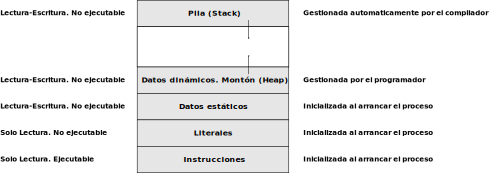
\includegraphics[width=0.3\textwidth]{img/memoria_2.png}
      \caption{Esquema de la memoria tras ejecutar dos asignaciones de números i32}
      \label{fig_memoria_2}
   \end{center}
\end{figure}

Este mecanismo de copia del valor en la nueva variable sucede siempre que los tipos implicados sean tipos primitivos y también con arrays y con tuplas de tipos primitivos. 

Observe, en cambio, el comportamiento cuando se hace un programa similar al anterior, pero en el que las variables son vectores:

\vspace{0.7em}
\begin{Codigo}
fn main() {
   let v = vec![10, 20];
   let w = x;
   println!("{:?}", w); // Imprime 10
   println!("{:?}", v); // ERROR, x no existe
}
\end{Codigo}

El programa anterior crea una variable \textit{v} de tipo \textit{Vec<i32>} y asigna valor a sus componentes. A continuación, crea una variable \textit{w} y le asigna el valor de \textit{v}. En asignaciones de este tipo, los vectores funcionan de manera diferente que los tipos primitivos (vea el esquema de la Figura \ref{fig_memoria_3}). 

Cuando se crea la variable \textit{w} y se le asigna el valor de \textit{v}, no se copia el valor de las componentes de \textit{v} en la nueva variable, lo que se asocia con la variable \textit{w} es la posición de memoria donde están guardadas las componentes del vector. En otros lenguajes, por ejemplo Java, a partir de ese momento habría dos variables en memoria, \textit{v} e \textit{w}, apuntando a la misma posición de memoria; se dice que Java \textit{asigna por referencia}, no por valor. En Rust, el funcionamiento es diferente: la variable \textit{w} se queda apuntando al valor, esto es, a la posición de memoria donde se guardan las componentes del vector, mientras que la variable \textit{v} queda inaccesible. Se dice que el valor de las componentes del vector se ha \textit{movido} de la variable \textit{v} a la variable \textit{w} o que la \textit{propiedad} del valor ha pasado de \textit{v} a \textit{w}.

La Figura \ref{fig_memoria_3} esquematiza este proceso. En la parte izquierda de la figura se muestra la situación tras la creación de la variable \textit{v}: se guarda la variable \textit{v} asociada a la posición de memoria en la que están almacenadas las componentes del vector, por ejemplo, la posición 5000. La parte derecha de la misma figura muestra la situación tras asignar a la variable \textit{w} el valor de la variable \textit{v}: la variable \textit{v} deja de existir y la propiedad del valor pasa a la variable \textit{w}\footnote{En realidad, la forma de asignar la memoria de un vector en Rust es un poco más compleja de lo que se esquematiza en la Figura \ref{fig_memoria_3}, pero a los efectos de la explicación del concepto de propiedad se ha considerado conveniente simplificarlo como se ha hecho.}.

\begin{figure}[htb]
   \begin{center}
      \includegraphics[width=\textwidth]{img/memoria_3.png}
      \caption{Izquierda: esquema de la memoria tras crear la variable \textit{v} del tipo \textit{Vec<i32>}. Derecha: esquema de la memoria tras asignar a la variable \textit{w} el valor de la variable \textit{v}}
      \label{fig_memoria_3}
   \end{center}
\end{figure}

En programación, se entiende por \textit{ámbito} de una variable (en inglés \textit{scope}) la parte del programa en la que dicha variable es accesible. En Rust, el ámbito de una variable lo determina el bloque en el que se crea la variable. Los bloques están delimitados entre dos llaves. Por ejemplo, en el siguiente código, la variable \textit{x} existe durante toda la extensión de la función \textit{main()}; en cambio, la variable \textit{y} solo existe dentro del bloque en el que se ha creado y cuando se intenta imprimir fuera de ese bloque, se produce un error.

\vspace{0.7em}
\begin{Codigo}
fn main() {
   let x= 10;
   {
      let y = 20;
   }
   println!("{:?}", x); // Imprime 10
   println!("{:?}", y); // ERROR, y no existe
}
\end{Codigo}

Las reglas por las que se rige el concepto de la \textit{propiedad de los valores} en Rust son las siguientes:

\begin{itemize}
   \item Cada valor tiene un propietario.
   \item En todo momento, cada valor tiene un solo propietario.
   \item Si se termina el ámbito del propietario, se destruyen el valor y el propietario.
\end{itemize}

Los tipos de datos que no están afectados por el concepto de propiedad se dice que se rigen por una semántica \textit{Copy}, mientras que los tipos que sí están afectados por el concepto de propiedad se dice que funcionan con semántica \textit{Move}.

\section{Referencias}
Es posible tomar prestada la propiedad de un valor utilizando una referencia al mismo. El compilador de Rust se encarga de comprobar que ninguna referencia sobreviva más allá que el valor al que apunta.

Hay dos tipos de referencias:

\begin{itemize}
   \item \textbf{Referencias inmutables (\&):} permiten utilizar el valor al que apuntan, pero no permiten modificarlo. Pueden existir al mismo tiempo varias referencias inmutables a un mismo valor en memoria.
   \item \textbf{Referencias mutables (\&mut):} permiten utilizar el valor al que apuntan y permiten también su modificación. Solo puede existir una referencia mutable a un valor en cada momento. Si durante la ejecución de un programa existe una referencia mutable a un valor en memoria, no pueden existir simultáneamente otras referencias al mismo valor, ni mutables ni inmutables.
\end{itemize}

Se denomina \textit{desreferenciar} a obtener el valor al que apunta una referencia. En muchas situaciones, Rust desreferencia directamente. Por ejemplo, si ejecuta el siguiente código, el valor que se imprime en pantalla es el valor al que apunta la referencia, no la referencia en sí misma:

\vspace{0.7em}
\begin{Codigo}
fn main() {
   let x = 32.6;
   let ref_x = &x;
   println!("{}", ref_x); // Imprime 32.6
}
\end{Codigo}

Hay ocasiones, no obstante, en que es necesario forzar la desreferenciación explícitamente. Para ello, se usa el operador $*$ (asterisco) colocado delante de la referencia, como se hace en el siguiente ejemplo:

\vspace{0.7em}
\begin{Codigo}
fn main() {
   let mut v = vec![10, 20, 30];
   for num in &mut v {
      if *num > 20 {
         *num = 40;
      }
   }
   println!("{:?}", v); // [10, 20, 40]
}
\end{Codigo}

Si se quiere imprimir la dirección de memoria a la que apunta una referencia, hay que utilizar la especificación de formato \textit{{:p}}:

\vspace{0.7em}
\begin{Codigo}
fn main() {
   let x = 32.6;
   let ref_x = &x;
   println!("{}", ref_x); // Imprime 32.6
   println!("{:p}", ref_x); // Imprime 0x7fff189f4bb8
}
\end{Codigo}



% -----------------------------------------------------------
\chapter{Funciones de orden superior, closures e iteradores}
\label{ch_funciones}
% -----------------------------------------------------------

\begin{Resumen}
En matemáticas y en ciencias de la computación, se denominan funciones de orden superior a las que cumplen al menos una de las siguientes condiciones:

\begin{itemize}
   \item Tomar una o más funciones como parámetro de entrada.
   \item Devolver una función como salida.
\end{itemize}

En matemáticas, un ejemplo lo podría constituir la función derivada, que toma una función como parámetro y devuelve otra función.

\smallskip

Las funciones de orden superior se han implementado en los lenguajes más conocidos, pero su uso es particularmente frecuente en la programación funcional. 

\smallskip

En programación funcional, las funciones son consideradas elementos de primera clase, esto es, pueden usarse como argumentos de otras funciones, como valores devueltos y también asignarse a un símbolo o variable. La mayoría de los lenguajes han adoptado ya esta premisa y dan un tratamiento de primera clase a las funciones.

\smallskip

En este capítulo se va a hablar de funciones, de cómo asignarlas a variables y de cómo  utilizarlas como argumento o como valor devuelto de otras funciones. También se hablará de las closures, que son un tipo especial de funciones definidas dentro de otras funciones, que pueden acceder al contexto en el que se han definido. Por último, se hablará de los iteradores y cómo encadenar procesos utilizando iteradores y funciones de orden superior.

\end{Resumen}

\section{Funciones de primera clase}
En programación, se denominan \textit{elementos de primera clase} a los elementos del lenguaje que se pueden asignar a variables y se pueden utilizar como argumentos o como valor devuelto por otras funciones.

No todos los elementos del lenguaje son elementos de primera clase. Por ejemplo, en muchos lenguajes, los operadores aritméticos como el $+$, el $-$ y otros, no son de primera clase. También sucede algo parecido con algunas construcciones, como los bucles o las bifurcaciones.

Es importante entender la diferencia entre el concepto de \textit{declaración} y el de \textit{expresión}. Un elemento de un lenguaje se considera que es una \textit{declaración} cuando no devuelve ningún valor; una \textit{expresión}, en cambio, es un elemento que devuelve un valor.

En los lenguajes funcionales se da prioridad a las expresiones que devuelven valores. Así se hace en Rust. Algunas construcciones que en otros lenguajes son declaraciones, en Rust son expresiones. Es el caso de las bifurcaciones \textit{if} o de los bucles \textit{loop, for} o \textit{while}, como se indicó en los apartados \ref{sec_bifurcaciones} y \ref{sec_bucles}. En cambio, el operador \textit{let} es una declaración que no devuelve ningún valor.

Se podría realizar un código como el siguiente:

\vspace{0.7em}
\begin{Codigo}
fn main() {
   let x = 2;
   println!("{}", suma(if x==2 {3} else {4}, 5));
   
   let mut n = 1;
   println!("{}", loop {
      n=n+1;
      if n>3 {
         break 10
      }
   });
}
fn suma(x: i32, y: i32) -> i32 {
   x+y
}
\end{Codigo}

En el programa anterior, se utiliza una bifurcación \textit{if} como argumento de la función \textit{suma()} y un bucle \textit{loop} como argumento de la macro \textit{println!()}. Observe que, en realidad, lo que se utiliza como argumento es el valor que devuelven dichas expresiones. 

Actualmente, numerosos lenguajes se han adherido a la línea marcada por los lenguajes funcionales y consideran las funciones como elementos de primera clase. Esto es, permiten que las funciones se puedan asignar a variables y se puedan utilizar como parámetros o como valor devuelto por otras funciones. En Rust, las funciones son objetos de primera clase.

Se denominan \textit{Funciones de primer orden} o también \textit{funciones ordinarias} aquellas en las que ni los parámetros ni el valor devuelto son otras funciones. Por contra, las \textit{Funciones de orden superior} son aquellas en las que o bien alguno de los parámetros o bien el valor devuelto son una función.

Hay varias maneras de definir funciones en Rust:

\begin{itemize}
   \item Dentro de un módulo o fichero \textit{.rs}, con la visibilidad que le corresponda y acceso a otras funciones y a sus variables locales .
   \item Dentro de otra función o bloque de código, con visibilidad restringida a dicho bloque y acceso a otras funciones, pero no a variables del contexto del bloque en el que se ha definido.
   \item Cómo función asociada a un tipo de datos personalizado, como es el caso de las estructuras y las enumeraciones.
   \item Como closure definida dentro de otra función o bloque de código. Su visibilidad estará restringida al bloque en el que se ha definido, pero las closures sí que tienen acceso a las variables existentes en el contexto del bloque en el que se haya definido. 
\end{itemize}

Ya se comentó este tema en el Apartado \ref{sec_funciones}. También se habló allí de los tres tipos de funciones que considera Rust, en función del uso que hacen de la propiedad de los parámetros: el tipo \textit{Fn}, para funciones ordinarias, el tipo \textit{FnMut}, para funciones con parámetros mutables y el tipo \textit{FnOnce} para funciones que solo se pueden invocar una vez.

\subsection{Asignación de funciones a variables}
Cualquiera de los tipos de funciones presentes en Rust se pueden asignar a una variable. Luego, se puede utilizar la variable como si fuera la función. 

El siguiente código asigna a una variable de nombre \textit{raiz2} la función \textit{sqrt} de los números \textit{f64}. Como resultado, la variable \textit{raiz2} es del tipo \textit{fn(f64) -> f64}, esto es, una función que recibe un argumento del tipo \textit{f64} y devuelve un valor \textit{f64}. Observe la forma de calcular la raíz cuadrada utilizando la variable así definida:

\vspace{0.7em}
\begin{Codigo}
fn main() {
   let raiz2  = f64::sqrt;
   let y = raiz2(4.0); // Equivale a 4.0f64.sqrt()
   println!("{}", y);
}
\end{Codigo}

Se podría asignar una función previamente codificada, como se hace en el siguiente código:

\vspace{0.7em}
\begin{Codigo}
fn main() {
   let f = saludo;
   f(); // Imprime Hola, ¿qué tal?
}
fn saludo() {
   println!("Hola, ¿qué tal?");
}
\end{Codigo}

En este caso, la variable \textit{f} es del tipo \textit{fn()}, esto es, del tipo de las funciones que no reciben argumentos y no devuelven ningún valor.

Las closures también se pueden asignar a variables, como se hace en el siguiente ejemplo:

\vspace{0.7em}
\begin{Codigo}
fn main() {
   let cuadrado = |x| {x*x};
   println!("{}", cuadrado(3.0)); // Imprime 9
}
\end{Codigo}

\subsection{Utilización de funciones como parámetros de otras funciones}
Observe el código siguiente:

\vspace{0.7em}
\begin{Codigo}
fn main() {
   let pi = std::f64::consts::PI;
   println!("{}", operador(f64::sin, pi/2.0)); // Imprime 1
   println!("{}", operador(f64::cos, pi)); // Imprime -1
   println!("{}", operador(|x| x*x, 4.0)); // Imprime 16
   println!("{}", operador(duplica, 5.0)); // Imprime 10
}
fn operador(f:fn(f64) -> f64, x: f64) -> f64 {
   f(x)
}
fn duplica(x: f64) -> f64 {
   x*2.0
}
\end{Codigo}

En el código anterior, la función \textit{operador} es una función de orden superior que se ha definido con la siguiente signatura:

{\centering \texttt{fn operador(f:fn(f64) -> f64, x: f64) -> f64} \par}

Cualquier función con un único parámetro del tipo \textit{f64} y que devuelve un valor del tipo \textit{f64}, se podrá utilizar como argumento en la llamada a \textit{operador}. La función \textit{operador} devolverá el resultado de aplicar la función \textit{f} que recibe como primer argumento al valor \textit{x} del tipo \textit{f64} que recibe como segundo argumento.


\subsection{Uso de funciones como valor devuelto por otras funciones}
En el siguiente código se define una función de orden superior llamada \textit{operador} que recibe un número entero como argumento. Si el valor recibido es mayor que cero, \textit{operador} devuelve la función \textit{f64::sin}; en caso contrario, devuelve la función \textit{f64::cos}.

\vspace{0.7em}
\begin{Codigo}
fn main() {
   let pi = std::f64::consts::PI;
   let seno = operador(3);
   println!("{}", seno(pi/2.0)); // Imprime 1
   let coseno = operador(-2);
   println!("{}", coseno(pi)); // Imprime -1
}
fn operador(n: i32) -> impl Fn(f64) -> f64 {
   if n>0 {f64::sin} else {f64::cos}
}
\end{Codigo}

Observe la utilización de la cláusula \textit{impl} para indicar el tipo de función que devuelve \textit{operador}:

{\centering \texttt{fn operador(n: i32) -> impl Fn(f64) -> f64} \par}

\section{Mónadas en Rust}
La mónadas son un patrón de diseño que permite encadenar cálculos. Se les ha denominado \textit{el operador punto y coma}. Hay dos mónadas de uso habitual en Rust: las enumeraciones \textit{Option} y \textit{Result}. 

La enumeración \textit{Option} tiene la siguiente declaración:

\vspace{0.7em}
\begin{Codigo}
   pub enum Option<T> {
      None,
      Some(T),
   }
\end{Codigo}

El tipo \textit{T} puede ser cualquiera. Es fácil definir un valor del tipo \textit{Option}. Por ejemplo, el siguiente código declara dos variables del tipo \textit{Option<u32>}, una con cierto valor y otra sin valor:

\vspace{0.7em}
\begin{Codigo}
   let n = Some(3);
   let m: Option<u32> = None; 
\end{Codigo}

Observe que, en el caso de la variable \textit{n} que sí tiene valor, el tipo de datos viene definido por el valor en sí, mientras que en el caso de la variable \textit{m} hay que especificr el tipo de datos del \textit{Option}.

Los métodos \textit{is\_some()} e \textit{is\_none()} permiten saber si determinada variables del tipo \textit{Option} es la variante \textit{Some} o la variante \textit{None}:

\vspace{0.7em}
\begin{Codigo}
   fn main() {
      let n = Some(3);
      let m: Option<u32> = None;
      assert!(n.is_some());
      assert!(m.is_none());
   }
\end{Codigo}

Cuando la variante de la variable es \textit{Some}, se puede extraer su valor con el método \textit{unwrap()}:

\vspace{0.7em}
\begin{Codigo}
   let n = Some(3);
   assert_eq!(n.unwrap(), 3);
\end{Codigo}

La función \textit{unwrap()} interrumpe la ejecución del programa con \textit{panic!} si la variante es \textit{None}. Por ello, se suele utilizar más el método \textit{unwrap\_or()}, que proporciona un valor del mismo tipo que el contenido en el \textit{Option} como valor devuelto en el caso de que la variante sea \textit{None}:

\vspace{0.7em}
\begin{Codigo}
   assert_eq!(Some("car").unwrap_or("bike"), "car");
   assert_eq!(None.unwrap_or("bike"), "bike");
\end{Codigo}

También existen unos métodos \textit{unwrap\_or\_else()} y \textit{unwrap\_or\_default()}, que puede consultar en la documentación del tipo \textit{Option}.

Es habitual utilizar el tipo \textit{Option} como resultados de funciones. Como se sabe, Rust no dispone de tipo \textit{null} ni de ningún mecanismo de excepciones para la gestión de errores. 

Suponga una función que reciba dos parámetros enteros y devuelva la división de uno entre el otro. En Java, la solución podría ser la siguiente:

\vspace{0.7em}
\begin{Codigo}
   public class Main {
      public static void main(String[] args) {
         dividir(3, 0);
      }
      static int dividir(int num, int den) {
         return num/den;
      }
   }
\end{Codigo}

En Java, si el denominador es cero, se lanzará una excepción. En principio hay dos posibilidades para gestionar una función de ese tipo: capturar la excepción o interceptar los denominadores cero. Tenga en cuenta que no se podría hacer que la función devuelva \textit{null} o \textit{Not A Number}, pues no existen para valores del tipo \textit{int}.

En Rust, en cambio, se puede imponer que la función \textit{dividir()} devuelva un \textit{Option<i32>} en lugar de un valor entero. El código podría ser el siguiente:

\vspace{0.7em}
\begin{Codigo}
   fn main() {
      let n = dividir(3, 0);
      assert_eq!(n, None);
   }
   fn dividir(num: i32, den: i32) -> Option<i32> {
      match den {
         0 => None,
         _ => Some(num/den)
      }
   }
\end{Codigo}

La ventaja de devolver resultados de funciones con \textit{Option} es más evidente cuando hay que encadenar varias funciones en las que una o más de ellas pueden devolver resultados no válidos. Por ejemplo, suponga que se quiere realizar el siguiente cálculo, operando con números en coma flotante:
\begin{equation}
   \frac{\sqrt{log(x)}}{y}   
\end{equation}

En Java, la función podría ser parecida a la siguiente:

\vspace{0.7em}
\begin{Codigo}
   public class Prueba {
      public static void main(String[] args) {
         double x = -10;
         double y = 0;
         System.out.println(f(x, y));
      }
      double f(double x, double y) {
         double z = Math.sqrt(Math.log(x)) / y;
         return z;
      }   
   }
\end{Codigo}

En la expresión anterior, si el valor de \textit{y} es cero y el numerador es distinto de cero, el resultado será \textit{Infinity}. También podría pasar que \textit{x} tuviera un valor negativo, en cuyo caso el logaritmo no existiría. Si el valor de \textit{x} no es negativo, pero es menor que \textit{1}, su logaritmo es negativo y la raíz cuadrada de un valor negativo devolvería \textit{Not A Number, NAN}. Como consecuencia, la función puede devolver un número del tipo \textit{double}, \textit{Infinity} o \textit{NaN}.

\begin{Nota}[Java online]
   \small
   Hay diversos portales online donde probar código Java. Si lo desea, puede probar el código anterior, dando diferentes valores a las variables \textit{x} e \textit{y}, en el siguiente enlace:
   
   {\centering \texttt{https://onlinegdb.com/2ea9z\_GhF} \par}
   
   \vspace{1em}
   
   Una vez en el portal, el código no es editable, pero puede pulsar el botón \textit{Fork} que aparece en la parte superior de la ventana para obtener la copia editable. 
\end{Nota}






\section{Pattern Matching}
In computer science, pattern matching is the act of checking a given sequence of tokens for the presence of the constituents of some pattern. 

Lexical tokenization is conversion of a text into (semantically or syntactically) meaningful lexical tokens belonging to categories defined by a "lexer" program. In case of a natural language, those categories include nouns, verbs, adjectives, punctuations etc. In case of a programming language, the categories include identifiers, operators, grouping symbols and data types. Lexical token consists of a token name and an optional token value. The token name is a category of a rule-based lexical unit. Ejemplos de tokens podrían ser los identificadores, las palabras clave del lenguaje, los separadores o símbolos de puntuación, los operadores, los literales, los comentarios y los espacios en blanco.

Por ejemplo, observe la siguiente expresión:

{\lstinline[language=Rust]!x = a + b;!}

El análisis lexicográfico daría lugar a los siguientes tokens:

{\lstinline[language=Rust]![(identifier, x),(operator, =),(identifier, a),(operator, +),(identifier, b),(separator, ;)]!}

\section{Patrones de programación funcional en Rust}
\begin{itemize}
   \item \textbf{Inmutabilidad:} se trata de una característica de la programación funcional que proporciona algunas ventajas: 
   \begin{itemize}
      \item Es más fácil razonar acerca del código, pues se tiene la seguridad de que no se van a producir cambios inesperados de los valores.
      \item Se pueden hacer optimizaciones como la \textit{memoization}, cacheando resultados.
      \item Simplifica la programación concurrente, ya que los valores inmutables se pueden compartir entre procesos sin tener que establecer bloqueos.
   \end{itemize}
   \item \textbf{Funciones puras:} son funciones que para unos mismos valores de entrada devuelven siempre el mismo resultado y que no tienen efectos secundarios de ningún tipo (no modifican estados globales ni modifican ningún datos fuera de su ámbito). Los beneficios de usar funciones puras son similares a los de la inmutabilidad: facilitan el razonamiento acerca del código y la depuración, facilitan la composición de funciones y permiten optimizaciones como la memoización o el paralelismo. 
   \item \textbf{Closures:} funciones anónimas que pueden capturar valores de su entorno.
   \begin{Codigo}
      let suma_uno = |x| x + 1;
   \end{Codigo}
   \item \textbf{Iteradores:} secuencias perezosas de elementos.
   \begin{Codigo}
      let v = vec![1, 2, 3];
      let double_v = v.iter().map(|x| 2 * x);
   \end{Codigo}
   \item \textbf{Funciones de orden superior:} funciones que se pueden pasar como parámetros o ser devueltas como resultados. 
   \begin{Codigo}
      fn square(x: i32) -> i32 {
         x * x
      }
      fn higher_order(f: fn(i32) -> i32, x: i32) -> i32 {
         f(x)
      }
      let result = higher_order(square, 10); // result is 100
   \end{Codigo}
   
   
   \item \textbf{Funciones como objetos de primera clase:} funciones de orden superior que se pueden usar como cualquier otro tipo de datos, asígnándolos a variables.
   \item \textbf{Coincidencia de patrones (\textit{Pattern matching}):} descomposición de estructuras.
   \begin{Codigo}
      let x = [1, 2, 3];
      match x {
         [1, _, _] => println!("{} {}", x[1], x[2]),
         _         => println!("El array no empieza por 1")
      }
   \end{Codigo}
   \item \textbf{Mónadas:} son un patrón de diseño que permite encadenar cálculos. Se les ha denominado \textit{el operador punto y coma}.
\end{itemize}

\section{Iteradores}
\label{sec_iteradorees}
Un \textit{Iterador} es un objeto que permite recorrer ordenadamente los elementos de una fuente de datos. En muchas ocasiones, la fuente de datos es una colección de objetos, pero también se pueden utilizar iteradores para leer ficheros línea a línea o para leer streams procedentes de un puerto de comunicaciones, por ejemplo.

Cuando un tipo de datos implementa el \textit{trait Iterator}, se convierte en una especie de colección, que es posible recorrer de manera ordenada. Por ello, es habitual referirse a los elementos de dicho tipo de datos como \textit{los elementos del iterador}, como si se tratase de una colección.

El uso de iteradores es un patrón de diseño muy utilizado en la programación funcional y que se ha incorporado progresivamente en todos los lenguajes de programación. Su origen se marca en el lenguaje CLU del año 1973 \citep{wikipediaCLUProgrammingLanguage2024}.

Técnicamente, un iterador en Rust es un tipo de datos que implementa el \textit{trait Iterator}, que impone la existencia del método \textit{next()}. Este método, si hay más elementos por iterar, devuelve \textit{Some(E)}, donde \textit{E} es el tipo de datos del iterador; si no quedan más elementos por iterar, devuelve \textit{None}.

Las colecciones que ofrece el lenguaje Rust ---arrays, vectores, hashmaps y otras--- permiten obtener un iterador sobre los elementos de la colección mediante el método \textit{into\_iter()}, o bien un iterador sobre referencias a los elementos de la colección utilizando el método \textit{iter()}. La diferencia fundamental entre ambos métodos es que, si se utiliza el método \textit{into\_iter()}, se \textit{consume} la colección, pasando la propiedad al proceso que la esté utilizando; el método \textit{iter()}, en cambio, utiliza referencias y no \textit{consume} la propiedad de la colección.

El siguiente ejemplo utiliza el método \textit{iter()} con un vector. Tras recorrer el vector, los elementos de la colección siguen estando disponibles:

\vspace{0.7em}
\begin{Codigo}
fn main() {
   let v = vec![1, 2, 3, 4, 5];
   for num in v.iter() {
      println!("{}", num);
   }
   println!("{}", v[0]);
}
\end{Codigo}

En cambio, si en el ejemplo anterior se utiliza el método \textit{into\_iter()}, se consume el vector en el bucle y los elementos de la colección ya no estarán accesibles después de la ejecución del mismo:

\vspace{0.7em}
\begin{Codigo}
fn main() {
   let v = vec![1, 2, 3, 4, 5];
   for num in v.into_iter() { // into_iter() mueve la propiedad
      println!("{}", num);
   }
   println!("{}", v[0]); // Error, v se movió al bucle
}
\end{Codigo}

Es posible utilizar un bucle \textit{for} para recorrer una colección sin llamar explícitamente a ninguno de los dos métodos. El problema será similar: si se recorre la colección, se pasa la propiedad al bucle, mientras que si se recorre utilizando una referencia, la colección no se consume en el bucle. 

El siguiente ejemplo utiliza una referencia a la colección y los elementos del vector siguen disponibles tras finalizar el bucle:

\vspace{0.7em}
\begin{Codigo}
fn main() {
   let v = vec![1, 2, 3, 4, 5];  
    
   for num in &v { // Se utiliza una referencia &v
      println!("{}", num);
   }
   println!("{}", v[0]); // v sigue disponible
}
\end{Codigo}

En cambio, en el siguiente ejemplo, el bucle utiliza directamente la colección y consume la propiedad de la misma. Al finalizar el bucle, no se puede acceder a los elementos de la colección:

\vspace{0.7em}
\begin{Codigo}
fn main() {
   let v = vec![1, 2, 3, 4, 5];      
   // Se recorre la colección, se pasa la la propiedad de v 
   for num in v {
      println!("{}", num);
   }
   // Ahora v ya no está disponible
   println!("{}", v[0]); // Error
}
\end{Codigo}

En Rust, al definir los iteradores, se hace referencia al tipo de elementos que recorre, pero no al tipo de colección o a la fuente de los datos que los alberga. Ésto permite definir funciones que describen la intención de lo que se quiere conseguir al procesar una fuente de datos, de manera independiente a la forma que adopten dichos datos. De esta forma, se podría cambiar la fuente de datos o su forma interna de organización, manteniendo las funciones que procesan dichos datos. Se trata de una codificación más declarativa que los bucles.

Los iteradores proporcionan numerosos métodos que permiten operar con los elementos que se iteran. Básicamente hay dos tipos de métodos:

\begin{itemize}
   \item Métodos que devuelven un nuevo iterador obtenido al realizar alguna operación sobre los elementos del iterador original. Se suelen llamar \textit{adaptadores} o también \textit{iteradores internos}. Ejemplos de estos métodos serían \textit{map()} y \textit{filter()}.
   \item Métodos que realizan alguna operación directamente sobre los elementos del iterador. Se suelen denominar \textit{iteradores externos}. Un ejemplo de estos métodos sería \textit{for\_each()}. 
\end{itemize}

Los métodos adaptadores permiten encadenar operaciones haciendo que la salida de cada uno ellos, sea la entrada del siguiente. Ésto favorece la \textit{canalización del procesamiento} de los datos (\textit{processing pipeline}). La codificación obtenida es declarativa y muestra de manera explícita qué se quiere hacer con los datos, en contra de lo que sucede al realizar el procesamiento a base de bucles.

La totalidad de los métodos que proporcionan los iteradores se pueden consultar en la documentación de la librería estándar, en la siguiente dirección:

{\centering\small \texttt{https://doc.rust-lang.org/std/iter/trait.Iterator.html} \par}

Una característica de los iteradores en Rust es que actúan de manera perezosa, esto es, las operaciones asociadas a sus métodos no se ejecutan hasta que son necesarias. En concreto, es habitual tras una serie de operaciones encadenadas utilizando los métodos del iterador, querer convertir el iterador resultante en algún tipo de colección, como un vector u otra. Para ello, se suele utilizar el método \textit{collect()}, que permite obtener una colección a partir de un iterador. En ese momento se ejecutarán las operaciones. En los ejemplos que siguen se verá cómo utilizar el método \textit{collect()} en diferentes situaciones.

Muchos de los métodos que se utilizan cuando se trabaja con iteradores son más o menos estándar y están disponibles en todos los lenguajes que hacen uso de iteradores, si bien, en algunos casos pueden utilizar nombres diferentes. 

Los métodos de los iteradores es frecuente que sean ejemplos paradigmáticos de funciones de orden superior: reciben una función como argumento que es la que se utilizará para operar sobre los elementos del iterador. También es frecuente que la función que se pasa como argumento sea una closure.

Tres de estos métodos que podríamos decir que son estándar en cualquier lenguaje que utilice iteradores son los métodos \textit{map}, \textit{filter} y \textit{fold}:

\begin{itemize}
   \item \textit{map()}: este método recibe como argumento una función que se aplica sobre cada uno de los elementos del iterador. El método \textit{map} devuelve un nuevo iterador cuyos elementos no tienen por qué ser del mismo tipo que los del iterador original.
   \item \textit{filter()}: recibe como argumento una función que al aplicarla a los elementos del iterador devuelve \textit{true} o \textit{false}. A esta función que recibe como argumento se le llama el \textit{filtro}. El método \textit{filter} devuelve un nuevo iterador con los elementos del iterador original en los que el filtro devuelve \textit{true}.
   \item \textit{fold()}: este método acumula los valores del iterador en un valor que puede ser de otro tipo diferente que el de los elementos del iterador. También utiliza una función como argumento. Es posible encontrar este método en otros lenguajes con el nombre \textit{reduce}. En Rust también hay un método \textit{reduce}, similar a \textit{fold()}. 
\end{itemize}

   
En los siguientes apartados se van a tratar en profundidad estos tres métodos.
   
\section{El método \textit{map()}}
Como se ha dicho, el método \textit{map()} recibe como argumento una función y la aplica a los elementos del iterador para obtener un nuevo iterador. La función que se pasa como argumento a \textit{map()}, toma como argumento un elemento del iterador original y devuelve otro elemento, que puede ser del mismo tipo o de otro. El resultado final es un nuevo iterador con elementos que no tienen por qué ser del mismo tipo que los del iterador original. La Figura \ref{fig_map} muestra el esquema de funcionamiento de \textit{map()}.

\begin{figure}[htb]
   \begin{center}
      \includegraphics[width=0.7\textwidth]{img/map.png}
      \caption{Esquema de funcionamiento de \textit{map()}}
      \label{fig_map}
   \end{center}
\end{figure}
      
En el siguiente código se crea un vector \textit{v} de números enteros y se obtiene un nuevo vector formado por los cuadrados de dichos números.

\vspace{0.7em}
\begin{Codigo}
fn main() {
   let v = vec![1, 2, 3, 4, 5];
   
   let iterador_original = v.into_iter();
   let new_iterador = iterador_original.map(|x| x*x);
   let new_vector: Vec<i32> = new_iterador.collect();
   
   println!("{:?}", new_vector); // Imprime [1, 4, 9, 16, 25]
}
\end{Codigo}

Observe los pasos que se han seguido:
\begin{enumerate}
   \item Se obtiene un iterador a partir del vector \textit{v} utilizando el método \textit{into\_iter()}.
   \item Se obtiene un nuevo iterador aplicando el método \textit{map} al iterador original. El método \textit{map} recibe como argumento una closure que, para cada valor \textit{x} del iterador original, devuelve su cuadrado.
   \item El iterador resultante de la aplicación de \textit{map()} se convierte de nuevo en un vector utilizando el método \textit{collect()}. Al método \textit{collect} hay que indicarle el tipo de colección que se quiere obtener, que en este caso es \textit{Vec<i32>}.
\end{enumerate}

Aunque en el ejemplo se ha desglosado cada paso para hacerlo más didáctico, lo habitual es hacer todas las operaciones encadenadas. También es habitual ir poniendo las sucesivas operaciones en diferentes líneas, utilizando la tabuladores para dar claridad al código. El siguiente ejemplo es equivalente al anterior:

\vspace{0.7em}
\begin{Codigo}
fn main() {
   let v = vec![1, 2, 3, 4, 5];
   
   let new_vector: Vec<i32> = v.into_iter() 
      .map(|x| x*x)
      .collect();
   
   println!("{:?}", new_vector); // Imprime [1, 4, 9, 16, 25]
}
\end{Codigo}

Como se ha dicho, el iterador resultante de la aplicación de \textit{map()} puede tener elementos de distinto tipo que el iterador original. En el siguiente ejemplo, el iterador original es de cadenas de caracteres y se obtiene un iterador con el número de caracteres de cada una de esas cadenas:

\vspace{0.7em}
\begin{Codigo}
fn main() {
   let v = vec!["Uno", "Dos", "Tres", "Cuatro", "Cinco"];
   
   let new_vector: Vec<i32> = v.into_iter()
      .map(|x| x.len() as i32)
      .collect();
   
   println!("{:?}", new_vector); // Imprime [3, 3, 4, 6, 5]
}
\end{Codigo}

\section{El método \textit{filter()}}
El método \textit{filter()} recibe como argumento un función de retorno lógico: \textit{true} o \textit{false}. El parámetro de la función es del tipo de los elementos del iterador. El resultado es un nuevo iterador formado por los elementos del iterador original que \textit{pasan el filtro}, esto es, los elementos en los que la función filtro devuelve \textit{true}. La Figura \ref{fig_filter} esquematiza el funcionamiento de \textit{filter()}.


\begin{figure}[htb]
   \begin{center}
      \includegraphics[width=0.7\textwidth]{img/filter.png}
      \caption{Esquema de funcionamiento de la función \textit{filter()}}
      \label{fig_filter}
   \end{center}
\end{figure}

El siguiente ejemplo parte de un vector de tuplas con las de dos coordenadas \textit{f64} de una serie de puntos. Se aplica un filtro para extraer los puntos del vector original que son interiores a un círculo de radio \textit{1} centrado en el origen.

\vspace{0.7em}
\begin{Codigo}
   fn main() {
      let v: Vec<(f64, f64)> = vec![
      (1., 1.), (0.5, -0.25), 
      (2., 0.1), (-0.5, -0.5)
      ];
      
      let new_vector: Vec<(f64, f64)> = v.into_iter()
         .filter(|(x, y)| (x * x + y * y).sqrt() < 1.0)
         .collect();
      
      println!("{:?}", new_vector); // [(0.5, -0.25), (-0.5, -0.5)]
   }
\end{Codigo}

Observe que en la función \textit{filter}, a diferencia de lo que ocurría con la función \textit{map()}, los elementos del iterador resultante son del mismo tipo que los del original. De hecho, son un subconjunto de los elementos del iterador original.

\section{El método \textit{fold()}}
El método \textit{fold()} aplica la función que recibe como argumento a los valores del iterador original, acumulando los valores en un solo valor que no tiene por qué ser del mismo tipo. A diferencia de \textit{map} y \textit{filter}, el método \textit{fold()} tiene dos parámetros: el valor inicial del acumulador y la función que se utilizará para realizar los cálculos. La signatura de \textit{fold()} es la siguiente:

{\centering \texttt{fn fold(valor\_inicial\_acumulador: B, f)-> B)} \par}

La función \textit{f} es del tipo \textit{FnMut}, recibe dos parámetros: el elemento del iterador original que se está procesando y un valor del tipo de datos \textit{B} del acumulado; la función debe devolver un valor del tipo de datos \textit{B} del acumulado. Llamando \textit{A} al tipo de datos de los valores del iterador original y \textit{B} al tipo de datos del valor acumulado, esto se puede expresar así:

{\centering \texttt{f: FnMut(B, T) -> B} \par}

Seguramente, un ejemplo ayude a comprender el funcionamiento de la función \textit{fold()} mejor que tanta explicación. El siguiente código, calcula la suma de los elementos de un vector de números enteros:

\vspace{0.7em}
\begin{Codigo}
fn main() {
   let v: Vec<i32> = vec![1, 2, 3, 4, 5];
   
   let suma: i32 = v.iter()
      .fold(0, |acc, x| acc+x);
   println!("{suma}"); // Imprime 15
}
\end{Codigo}

Observe que, en este caso, el valor inicial del acumulador es \textit{0}. La función acumuladora declara dos parámetros: \textit{acc} y \textit{x}. En cada iteración, \textit{acc} contendrá el actual valor del acumulador. La función devuelve la suma de \textit{acc} y \textit{x}. 

Observe también que, para obtener el iterador del vector, se ha utilizado el método \textit{iter()}, por lo que las \textit{x} de la función acumuladora son referencias a los valores del vector original y no se consume el vector.

La variable \textit{acc} que se utiliza para el acumulador necesita ser mutable, de ahí que se haya dicho que la función acumuladora es del tipo \textit{FnMut}.

En el siguiente ejemplo, los valores del iterador original son del tipo \textit{char}, mientras que el valor acumulado es del tipo \textit{String}:

\vspace{0.7em}
\begin{Codigo}
fn main() {
   let v: Vec<char> = vec!['h', 'o', 'l', 'a'];
   
   let suma: String = v.into_iter()
      .fold(String::new(), |mut acc, c| {
            acc.push(c);
            acc
         }
      );
   println!("{suma}"); // Imprime hola
}
\end{Codigo}

En este caso, ha sido necesario declarar que el parámetro \textit{acc} de la closure es mutable. También ha sido necesario operar en dos pasos, pues la función \textit{push()} modifica la cadena original pero devuelve el valor unitario \textit{()}.

Otro ejemplo clásico es el cálculo del máximo de una serie de números:

\vspace{0.7em}
\begin{Codigo}
fn main() {
   let v: Vec<i32> = vec![-1, 2, 5, 1, -2];
   
   let maximo: i32 = v.iter()
      .fold(v[0], |acc, x | if *x>acc {*x} else {acc});
   println!("{}", maximo); // Imprime 5
}
\end{Codigo}

Un ejemplo un poco más complejo podría ser el calculo de la longitud de una polilínea definida mediante las coordenadas de sus puntos:

\vspace{0.7em}
\begin{Codigo}
fn main() {
   let v: Vec<(f64, f64)> = vec![(0., 0.), (1., 1.), (2., 2.)];
   
   let acumulado: (f64, f64, f64) = v.iter()
      .fold((v[0].0, v[0].1, 0.0), |acc, p |{
         let d = ((p.0 - acc.0)*(p.0 - acc.0) + 
                  (p.1 -acc.1)*(p.1 -acc.1)).sqrt();
         (p.0, p.1, acc.2 + d)
      }
   );
   println!("{:.4}", acumulado.2); // Imprime 2.8284
}
\end{Codigo}

Observe que, en este caso, cada iteración necesita las coordenadas del punto anterior, de ahí la técnica que se ha utilizado para definir los valores acumulados como una tupla de tres componentes.




\subsection{Ejemplo: cálculo del máximo}


\section{Herramientas de los Iteradores}




Rust ofrece otras funciones que se pueden aplicar a los iteradores. 

\begin{itemize}
   \item \textbf{for\_each():} devuelve la lista resultante de aplicar la closure que recibe como argumento a cada elemento de la lista original. Es equivalente a un bucle \textit{for}, aunque en determinadas situaciones puede ser más rápido.
   
   \item \textbf{filter():} devuelve la lista resultante de filtrar los elementos de la lista original utilizando para ello la closure que recibe como argumento. La closure acepta como parámetro un elemento del tipo de datos de los elementos de la lista y devuelve \textit{true} o \textit{false}. La lista resultante contendrá solo los elementos en los que la closure devuelva \textit{true}.
   
   El siguiente ejemplo extrae los elementos pares del array original:
   \vspace{0.7em}
   \begin{Codigo}
      fn main() {
         let lista = [1, 2, 3, 4, 5];
         let nueva_lista: Vec<&i32> = lista.iter().filter(|&x| *x%2==0).collect();
         println!("{:?}", nueva_lista); // [2, 4]
      }
   \end{Codigo}
   En el ejemplo anterior, la función \textit{filter()} opera sobre un iterador de referencias a valores, por lo que primero hay que convertir el array original en un iterador de referencias a números enteros usando el método \textit{iter()}. La closure recibe una referencia a un elemento como parámetro, \textit{\&x}, y comprueba si el resto de dividir por 2 el valor al que apunta dicha referencia es igual a 0. Sucede que, a priori, no se conoce el tamaño del array resultante y el tamaño de un array hay que conocerlo en tiempo de compilación, por lo que se utiliza el método \textit{collect()} para convertir el iterador resultante en un vector de referencias a números enteros.  
   
   
   
   \vspace{0.7em}
   \begin{Codigo}
      
   \end{Codigo}
\end{itemize}



La totalidad de las funciones aplicables a los iteradores se pueden consultar en el siguiente enlace:

{\centering \url{} \par}

(Fuentes: 
\begin{itemize}
   \item \url{https://blog.jetbrains.com/rust/2024/03/12/rust-iterators-beyond-the-basics-part-i-building-blocks/})
   \item Module iter: \url{https://doc.rust-lang.org/std/iter/}
   \item Processing a Series of Items with Iterators: \url{https://doc.rust-lang.org/book/ch13-02-iterators.html}
   \item \url{https://mustafabugraavci.blog/2024/04/23/mastering-iterators-in-rust-enhancing-performance-and-productivity/}
   
\end{itemize}



% -------------------------------------------
\chapter{Funciones puras, inmutabilidad}
\label{ch_funciones_puras}
% -------------------------------------------

\IndiceCapitulo

\begin{Resumen}
   Como se indicó en el Capítulo \ref{ch_intro}, una de las características distintivas de la Programación Funcional es su preferencia por la utilización de las \textit{funciones puras}, esto es, funciones sin efectos secundarios. Algunos autores utilizan la denominación \textit{cálculos}, para referirse a las funciones puras y \textit{acciones}, para referirse a las funciones con efectos secundarios \citep{normandGrokkingSimplicityTaming2021}. Esta será la denominación que se utilizará preferentemente en el texto a partir de este momento.
   
   \smallskip
   
   Otro de los pilares de la programación funcional es la utilización de las estructuras de datos inmutables, lo que proporciona ventajas a la hora de hacer determinadas optimizaciones en el código compilado y facilita la programación concurrente y en paralelo. 
   
   \smallskip
   
   En este capítulo se va a ahondar en la utilización de las funciones puras y variables inmutables. Las técnicas que se van a explicar, que proceden en su mayoría de patrones de diseño de la Programación Funcional, no dependen del lenguaje de programación que se utilice y su aplicación  produce beneficios al código generado, haciéndolo más fácil de comprender, favoreciendo su reutilización y facilitando el proceso de pruebas y depuración. Se pueden aplicar por igual a la programación orientada a objetos o a la programación basada en procedimientos. En realidad, se podría decir que se trata simplemente de buenas prácticas de programación.
   
   \smallskip
   
   Hay dos ideas principales que subyacen en todas estas técnicas:
   
   \begin{itemize}
      \item Separar las acciones de los cálculos y de los datos.
      \item Propiciar el uso de abstracciones de orden superior.
   \end{itemize}
    
\end{Resumen}

\section{Distinguir entre datos, cálculos y acciones}
El código de los programas se puede dividir en tres categorías: 

\begin{itemize}
   \item Datos.
   \item Cálculos (funciones puras, funciones sin efectos secundarios).
   \item Acciones (funciones impuras, funciones con efectos secundarios).
\end{itemize}

Los \textit{datos} son la plasmación de hechos que han sucedido. Los datos no producen efectos secundarios ni dan lugar a ningún resultado. Son código inerte. Lo que sí admiten, son diferentes interpretaciones. Un mismo dato, por ejemplo una cadena de texto con una palabra, puede admitir diferentes interpretaciones según el programa concreto que haga uso de ella.

Las \textit{funciones puras} son aquellas que no producen efectos secundarios, no dependen de ningún estado exterior y siempre proporcionan el mismo resultado para el mismo valor de los argumentos de entrada (ver Figura \ref{fig_funcion_pura}). Se suelen denominar también \textit{funciones matemáticas} o \textit{cálculos}. En este texto, siguiendo la denominación utilizada por Eric Normand, se denominarán frecuentemente \textit{cálculos} \citep{normandGrokkingSimplicityTaming2021}.

\vspace{0.7em}
\begin{figure}[htb]
   \begin{center}
      \includegraphics[width=0.75\textwidth]{img/funcion_pura.png}
      \caption{Funciones puras y efectos secundarios.}
      \label{fig_funcion_pura}
   \end{center}
\end{figure}

Se entiende por \textit{efecto secundario} cualquier acción del programa que no sea un cálculo. Por ejemplo, modificar el estado de una variable, mostrar un mensaje en una pantalla o enviar un correo electrónico serían ejemplos de efectos secundarios. Cuando una función produce algún efecto secundario, se dice que es una \textit{función impura}, una \textit{función con efectos secundarios} o, siguiendo la denominación de Eric Normand, una \textit{acción}. Así se denominarán frecuentemente en el texto a partir de ahora.

No es posible hacer un programa de utilidad sin producir efectos secundarios. De hecho, los efectos secundarios suelen ser la razón de ser de los programas. Lo que sí se puede hacer es codificar los programas de forma que las acciones siempre se lleven a cabo dentro de ámbitos controlados y bajo una supervisión minuciosa.

Al inspeccionar cualquier fragmento de código, hay que distinguir las partes que son acciones, de las que son cálculos y de las que son simplemente datos. En general, se debe dar preferencia a la utilización de datos sobre los cálculos y a los cálculos sobre las acciones.

\pagebreak

Un ejemplo de cálculo sería la función siguiente:

\vspace{0.7em}
\begin{Codigo}
fn cuadrado(x: f64) -> f64 {
   x*x
}
\end{Codigo}

La función anterior, recibe como argumento un número del tipo \textit{f64} y devuelve el cuadrado de dicho número. El código dentro de la función no afecta a nada externo a la misma, no tiene ninguna entrada de información que no sea a través de su parámetro ni ninguna salida que no sea a través de su valor devuelto; el valor que devuelve, siempre será el mismo si recibe el mismo valor como argumento, independientemente de en qué momento se llame a la función o cuántas veces se llame a la misma. 

Las acciones, en cambio, son funciones con efectos secundarios. Los efectos secundarios pueden tomar distintas formas dentro del código. Por ejemplo:
\begin{itemize}
   \item Llamadas a otras funciones o métodos: \texttt{println!("Hola, qué tal")}   
   \item Constructores: \texttt{new Date()}
   \item Expresiones: \texttt{x} (si \texttt{x} es mutable).   
   \item Declaraciones: \texttt{x = 3} (si se muta \texttt{x}).
\end{itemize}

Las funciones que son acciones, pueden estar compuestas por otras acciones, cálculos y datos. Una función que sea un cálculo puede estar compuesta por varios cálculos menores. Los datos solo pueden contener otros datos.

A continuación, se van a explicar con más detalle las características de los datos, los cálculos y las 
acciones.

\subsection{Datos}
Los datos son hechos resultantes de acontecimientos que han sucedido a lo largo de la ejecución del programa. Sus características principales son las siguientes:
\begin{itemize}
   \item Se implementan utilizando los tipos de datos que ofrezca el lenguaje de programación que se esté utilizando.
   \item Las estructura de los datos encierra parte de su significado, por ejemplo, el orden de los elementos en una lista.
   \item Los datos en sí mismos, son inmutables. Los datos de un acontecimiento no varían, lo que puede suceder es que se produzcan nuevos acontecimientos que den lugar a nuevos datos.
   \item \textit{Ventajas de los datos:} son serializables, se pueden comparar para comprobar su igualdad, están abiertos a distintas interpretaciones.
   \item \textit{Desventajas:} el hecho de que admitan distintas interpretaciones puede ser un arma de doble filo. Un cálculo es útil, aunque no entendamos cómo está hecho, pero un dato no tiene ningún significado sin una interpretación adecuada.
\end{itemize}

En los programas, conviene separar la generación de los datos de su utilización. Por ejemplo, si un programa tiene que enviar unos correos a una serie de personas, conviene proceder primero a generar los correos, guardarlos en una estructura de datos y luego enviarlos. 

Es preferible hacerlo así, que ir generando los correos uno a uno e ir enviando cada correo que se genera. Esto, facilitará la realización de test: es más fácil probar una función que genera una lista de datos que una función que envía un correo.

Si la lista de correos fuera muy grande, siempre se podría repetir el procedimiento anterior dividiendo en subgrupos los correos que se tienen que enviar.

\subsection{Cálculos: funciones puras}
Los cálculos son las funciones  puras, también llamadas funciones matemáticas. A partir de una entrada se genera una salida. En una función que sea un cálculo, la entrada se produce a través de los parámetros de la función, la salida es el valor que devuelve y el cálculo es el cuerpo de la función. 

Los cálculos gozan de \textit{trasparencia referencial}, esto es, en cualquier lugar del código en el que aparece la llamada a una función que es un cálculo, se puede sustituir dicha llamada por el resultado que se obtiene. Cuando el compilador identifica un cálculo, puede proceder a optimizaciones sustituyendo la llamada a la función por su resultado. Esto no es posible garantizarlo en el caso de que la función sea una acción. 

Las características de los cálculos:

\begin{itemize}
   \item En los programas, los cálculos se implementan utilizando funciones.
   \item El significado que encierran es el cálculo que hacen.
   \item Las ventajas de los cálculos frente a las acciones son:
   \begin{itemize}
      \item Es más fácil hacer test y probarlos.
      \item Los test se pueden automatizar más fácilmente.
      \item Es posible componer unos cálculos con otros.
      \item No hay que preocuparse de otros cálculos que se pudieran estar produciendo al mismo tiempo, el resultado solo depende del valor de los argumentos de entrada (programación en paralelo).
      \item Por el mismo motivo, no hay que preocuparse de lo que haya sucedido antes de llamar al cálculo o de lo que pueda suceder después.
      \item No hay que preocuparse de cuántas veces se haya llamado anteriormente al cálculo.
   \end{itemize}
   \item \textit{Desventajas:} al igual que sucede con las acciones, no se  puede estar seguro de lo que hacen si no se ejecuta el código. Lo único que se está seguro de lo que hacen son los datos, que no hacen nada.
\end{itemize}

\subsection{Acciones: funciones con efectos secundarios}
Las funciones que tienen entradas o salidas implícitas, son \textit{acciones}, también llamadas \textit{funciones con efectos secundarios} o \textit{funciones impuras}. Una acción es cualquier cosa que tenga un efecto en el mundo exterior a la función o que sea afectada por el mundo exterior. 

Sus características principales son:

\begin{itemize}
   \item Las acciones se implementan en el código utilizando funciones.
   \item Se propagan por el código: si una función llama a otra función que es una acción, ella misma se convierte en una acción.
   \item Las acciones dependen o pueden depender de cuándo se ejecutan (del orden de ejecución) o de cuantas veces se ejecutan (repetición).
   \item El significado de las acciones es el efecto que producen en el mundo exterior. Hay que asegurarse de que producen el efecto deseado.
   \item Las acciones son inevitables. De hecho, son la razón de ser de los programas.
\end{itemize}

La Programación Funcional propone diversas técnicas para gestionar de manera adecuada las acciones:
\begin{itemize}
   \item Reducir el número de acciones a las estrictamente necesarias.
   \item Mantenerlas reducidas a su mínima expresión, extrayendo de ellas todos los elementos que sean cálculos o datos.
   \item Restringir las acciones a las interacciones con el exterior. En el interior, idealmente, todo son cálculos y datos.
   \item Reducir la dependencia del tiempo. Hacer que las acciones dependan menos de cuándo se jecutan o de cuántas veces se ejecutan.
\end{itemize}

\section{Tipos de entradas y salidas de las funciones}
Todas las funciones tienen entradas y/o salidas. Se pueden clasificar en implícitas y explícitas:

\begin{itemize}
   \item \textit{Entradas explícitas}: a través de los parámetros.
   \item \textit{Salidas explícitas}: a través del valor devuelto.
   \item \textit{Entradas o salidas implícitas}: cualquier otra forma de entrada o salida de información de la función. 
\end{itemize}

Las entradas \textit{explícitas} son los valores de los argumentos que recibe la función. Cualquier otra entrada de información a la función se considera una entrada \textit{implícita}. Las salidas \textit{explícitas} son los valores devueltos. Cualquier otra salida de información de la función se considera una salida \textit{implícita} (ver Figura \ref{fig_funcion_pura}).

La existencia de entradas o salidas implícitas convierten una función en impura. Una \textit{entrada implícita} puede ser leer el valor de una variable externa a la función, por ejemplo una variable global. También sería un entrada implícita la consulta de datos provenientes de una base de datos. Las \textit{salidas implícitas} son cualquier información que salga de la función y que no sea el valor devuelto, por ejemplo, modificar el valor de una variable externa o enviar un email o escribir informacion en una base de datos o un fichero.

Cualquier entrada o salida implícita de información a la función convierte la función en impura, en una acción. 

Si en una función se eliminan todas las entradas y salidas implícitas, se convierte en un cálculo. Las entradas implícitas, hay que convertirlas en parámetros y las salidas implícitas hay que convertirlas en valores devueltos.

\section{Separar las cosas}
Conviene recordar el concepto de \textit{refactorizar}. Consiste en hacer modificaciones en el código organizándolo de otra manera sin alterar su comportamiento. Hay diversas técnicas de refactorización que se han estandarizado, por ejemplo, la denominada \textit{extraer subrutina} consiste en extraer una parte de una función a otra función independiente.

En general, la refactorización da lugar a un código con más líneas, pero es más comprensible, más reusable y es más fácil hacer los test.

Una técnica de diseño reconocida consiste en \textit{separar las cosas} (\textit{pull things apart}). Ésta técnica también es conocida como el \textit{Principio de Responsabilidad única}:  que cada función haga solo una cosa y que la haga bien. Da lugar a un código con más funciones y más pequeñas, pero facilita la reutilización y hace el código más fácil de comprender. En la Programación Funcional se promueve la utilización de funciones más pequeñas, separando las cosas. Los procesos complejos se consiguen mediante la \textit{composición} de dichas funciones. La figura \ref{fig_composicion_1} trata de esquematizar está técnica.

\begin{figure}[htb]
   \begin{center}
      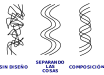
\includegraphics[width=0.55\textwidth]{img/composicion_1.png}
      \caption{Visualización de la separación de diferentes cosas y su composición}
      \label{fig_composicion_1}
   \end{center}
\end{figure}

\section{Extraer los cálculos de las acciones}
Observe la función \textit{grabar\_caudal()} que se muestra en el siguiente fragmento de código:

\vspace{0.7em}
\begin{Codigo}
fn grabar_caudal() {
   let velocidad = leer_sensor();
   let caudal = 1.8 * velocidad.powf(3.2);
   save_caudal_to_database(caudal);
}
\end{Codigo}

La función lee el valor de la velocidad de un sensor, realiza el cálculo del caudal asociado a esa velocidad y graba el resultado en una base de datos. La función es una acción: no tiene ningún argumento de entrada ni devuelve ningún resultado, pero tiene una entrada de datos implícita a través de la función \textit{leer\_sensor()} y una salida de datos implícita que graba datos en la base de datos utilizando la función \textit{save\_caudal\_to\_database()}.  

Además, la función incluye un cálculo, que aquí se ha expresado mediante una operación relativamente sencilla, pero que podría ser más complicado. 

Si se quisiera hacer algún test para comprobar que el cálculo se realiza de manera correcta, no sería fácil. Una opción sería habilitar el sensor correspondiente y la base de datos asociada mientras se hacen los test. Para comprobar que el resultado calculado es correcto, seguramente habría que consultar el valor grabado en la base de datos, pues la función no devuelve ningún valor. Si se quisiera probar el cálculo con diferentes valores de velocidad, habría que \textit{trucar} el sensor, lo que puede resultar complicado.

El problema está en que se están mezclando dos cosas: una acción (en ralidad, dos) y un cálculo. La solución adecuada es extraer el cálculo a una función independiente, como se muestra en el siguiente código:

\vspace{0.7em}
\begin{Codigo}
fn grabar_caudal() {
   let velocidad = leer_sensor();
   
   let caudal = calcula_caudal(velocidad);
   
   save_caudal_to_database(caudal);
}
fn calcula_caudal(velocidad: f64) -> f64 {
   let resultado = 1.8 * velocidad.powf(3.2);
   resultado
}
\end{Codigo}

Ahora hay dos funciones: una acción y un cálculo. Es fácil realizar los test para comprobar que los cálculos se hacen de manera adecuada. Se puede probar la función \textit{calcula\_caudal()} para cualquier valor de entrada de manera sencilla.

Los pasos que se han seguido se podrían esquematizar de la siguiente forma:
\begin{itemize}
   \item En la función original, seleccionar el fragmento de código a extraer.
   \item Ponerlo en una nueva función, sustituyéndolo en la función original por una llamada a la función recién creada. Es posible que haya que añadir algún parámetro.
   \item Identificar todas las entradas y salidas en la nueva función, convirtiendo las entradas en parámetros y las salidas en valores devueltos, que habrá que asignar a alguna variable en la función original.
   \item Los argumentos y lo valores devueltos de la función recién creadas tienen que ser inmutables, de forma que la nueva función sea un cálculo.
\end{itemize}

\section{Ejemplo: eliminar entradas implícitas}
En numerosas ocasiones, una misma función hace más de una cosa. Suponga que se tiene la siguiente función:

\vspace{0.7em}
\begin{Codigo}
fn main() {
   facturar(100.0);
}
fn facturar(precio: f64) {
   let descuento = 0.10 * precio;
   println!("Precio      : {:.2}", precio);
   println!("Descuento   : {:.2}", descuento);
   println!("Precio neto : {:.2}", precio - descuento);
}
\end{Codigo}

La función \textit{facturar()} recibe como argumento el precio de un artículo, calcula el descuento a aplicar y muestra el resumen de la factura en pantalla. Está haciendo dos cosas: calcular el descuento y mostrar los resultados en pantalla. El hecho de mostrar los resultados en pantalla es un efecto secundario, una salida implícita que convierte a la función en una acción. Pero, además, tiene una entrada implícita de información. El valor $0.10$ del porcentaje de descuento que se aplica es una especie de variable global, correspondiente a la lógica de negocio de la aplicación.

No es posible eliminar la acción, de hecho, es el objetivo del programa: mostrar la factura en pantalla, una vez que se ha aplicado el descuento. Es difícil diseñar un test para probar la función. Por una parte hay que probar que los cálculos son correctos y, por otra, que la salida de la función también es correcta. Tenga en cuenta que, aunque la salida se ha planteado simplemente mostrando unos mensajes en pantalla, podría tratarse de la actualización de ciertos registros en una base de datos o cualquier otra salida. En el caso de hacer la salida a una base de datos, para probar los cálculos, habría que habilitar y tener disponible la base de datos.

Lo correcto es separar el cálculo del descuento de la salida de resultados. Pero, además, la entrada implícita del porcentaje de descuento hay que convertirla en un parámetro de la función que calcula el descuento. Podría hacerse de la siguiente forma:

\vspace{0.7em}
\begin{Codigo}
fn main() {
   let porcentaje_descuento = 0.10;
   let precio = 100.0;
   let descuento = 
       calcula_descuento(precio, porcentaje_descuento);
   facturar(precio, descuento);
}
fn calcula_descuento(precio: f64, porcentaje: f64) -> f64 {
   precio*porcentaje
}
fn facturar(precio: f64, descuento: f64) {
   println!("Precio      : {:.2}", precio);
   println!("Descuento   : {:.2}", descuento);
   println!("Precio neto : {:.2}", precio - descuento);
}
\end{Codigo}

Ahora, la función \textit{calcula\_descuento()} es una función pura, un cálculo. Sus únicas entradas se producen a través de los argumentos que recibe y su salida es el valor que devuelve. No importa cuándo se llame a la función o cuántas veces se la llame: si recibe los mismos argumentos siempre devolverá el mismo resultado. Es fácil plantear los test para probar que realiza los cálculos de manera adecuada. 

Además, el porcentaje del descuento que se tiene que aplicar se ha independizado de cualquiera de las funciones. Está centralizado en una variable accesible para otras funciones del programa. Si la empresa decidiera cambiar su política de descuentos, solo tendría que modificar el valor de la variable en un sitio y se actualizaría la política en cualquier función que haga uso de ella.

Por otra parte, la función \textit{facturar()} sigue siendo una acción, pero independiente de otras consideraciones. Si se decidiera cambiar la forma de salida de la pantalla a una base de datos, por ejemplo, solo habría que actuar en dicha función, despreocupándose del cálculo de los valores asociados. Aun siendo una acción, se han eliminado sus entradas implícitas, convirtiéndolas en parámetros.

En el ejemplo, se han realizado varias refactorizaciones:
\begin{itemize}
   \item Extraer un cálculo de una acción.
   \item Convertir una entrada implícita en un parámetro.
   \item Separar las cosas en funciones independientes.
\end{itemize}

\section{Inmutabilidad. Copy-on-write}

Al inicializar una variable, se cambia su valor. Si en las funciones solo se inicializan variables locales, nada fuera de la función ve dichos cambios, salvo que lo vean a través del valor devuelto. 

Ejemplo sin copy-on-write:

\vspace{0.7em}
\begin{Codigo}
   fn main() {
      let mut list = vec![1, 2, 3];
      list.push(4);
      assert_eq!(list, vec![1, 2, 3, 4]);
   }
\end{Codigo}

Sin copy-on-write, pero con función:

\vspace{0.7em}
\begin{Codigo}
   fn main() {
      let mut list = vec![1, 2, 3];
      modify_list(&mut list, 4);
      assert_eq!(list, vec![1, 2, 3, 4]);
   }
   fn modify_list(list: &mut Vec<i32>, x: i32) {
      list.push(x);
   }
\end{Codigo}

Con copy-on-write:

\vspace{0.7em}
\begin{Codigo}
   fn main() {
      let list = vec![1, 2, 3];
      let list = copy_on_write(list, 4);
      assert_eq!(list, vec![1, 2, 3, 4]);
   }
   fn copy_on_write(list: Vec<i32>, x: i32) -> Vec<i32> {
      let mut new_list = list;
      new_list.push(x);
      new_list
   }
\end{Codigo}

No se modifica la lista original, se transforma en una nueva lista que incorpora las modificaciones. No hay pérdida de rendimiento, la propiedad de los valores se va trasmitiendo, sin modificar su posición en memoria.

Variante usando un \textit{RefCell}:

\vspace{0.7em}
\begin{Codigo}
   fn main() {
      let list = RefCell::new(vec![1, 2, 3]);
      let list = modify_cell(list, 4);
      assert_eq!(list.take(), vec![1, 2, 3, 4]);
   }
   fn modify_cell(list: RefCell<Vec<i32>>, x: i32) 
   -> RefCell<Vec<i32>> {
      let new_list = list;
      new_list.borrow_mut().push(x);
      new_list
   }
\end{Codigo}

\vspace{0.7em}
\begin{figure}[htb]
   \begin{center}
      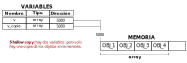
\includegraphics[width=0.8\textwidth]{img/shallow_copy.png}
      \caption{Esquema del mecanismo \textit{shallow-copy} de un \textit{array} en Java: se copian las referencias a los objetos, no los objetos en sí mismos. Al final hay dos variables apuntando a los mismos objetos en memoria.}
      \label{fig_shallow_copy_1}
   \end{center}
\end{figure}


\chapter{Colecciones}




\chapter{Patrones de diseño en la Programación Funcional}






\chapter{Grokking Simplicity}

\IndiceCapitulo

\begin{Resumen}   
   {\color{blue}Apuntes del Libro <<Grokking Simplicity>>, de Eric Norman \citep{normandGrokkingSimplicityTaming2021}}
\end{Resumen}

\section{Welcome to Grokking simplicity}

\section{Functional thinking in action}

\section{Distinguishing actions, calculations and data}

Los programadores funcionales clasifican cualquier fragmento de código como acción, cálculo o datos. Esta clasificación puede recibir otras denominaciones, pero el concepto es el mismo. 

\begin{itemize}
   \item \textbf{Acciones:} son todo aquello que dependa de en qué momento se ejecuta o de cuántas veces se ejecuta. Por ejemplo, enviar un correo es una acción.
   \item \textbf{Cálculos:} son las tareas que solo dependen de los valores de entrada para generar un resultado. Los cálculos siempre devuelven el mismo resultado, si los valores de entrada son los mismos. Además, los cálculos nunca afectan a nada que esté fuera de ellos. Esto hace que los cálculos sean fáciles de testear y que su uso sea seguro, pues no hay que preocuparse de cuántas veces se utilicen o en qué orden sean invocados: si los parámetros de entrada son los mismos, el resultado será siempre el mismo.
   \item \textbf{Datos:} los datos son información registrada acerca de los acontecimientos. Tienen propiedades conocidas. Un mismo dato se puede interpretar de manera diferente según el contexto de ejecución en el que se encuadra. Por ejemplo, la factura de una cena la puede utilizar el cliente para llevar la cuenta de sus gastos mensuales o la puede utilizar el propietario del restaurante para determinar los gustos favoritos de sus clientes.
\end{itemize}

\begin{figure}[htb]
   \centering
   \includegraphics[width=0.7\linewidth]{img/AccCalcData.png}
   \caption{Ejemplos de código: Acciones, Cálculos y Datos}
   \label{fig_acccalcdata}
\end{figure}


La proliferación de los sistemas distribuidos en los que intervienen diferentes dispositivos y peticiones cuasi simultáneas de información a las bases de datos, el problema de organizar de manera adecuada el código se hace indispensable. En general, el código de las acciones será más difícil de comprender y de testear que el código de los cálculos, ya que estos últimos no dependen del número de veces que se invocan o del orden de dichas invocaciones. Es por ello que se hace importante separar en la medida de los posible el código que corresponde a las acciones del código que corresponde a los cálculos.

La programación funcional proporciona herramientas para el correcto tratamiento de cada una de estas categorías de código. En el caso de las acciones, es importante gestionar la forma en que cambia el estado de las variables del programa a lo largo del tiempo, garantizando el número de veces y el orden en el que se realiza cada acción. Los cálculos tienen su propia estrategia para comprobar su buen funcionamiento, a veces basada en técnicas matemáticas. En el caso de los datos, es importante organizarlos en estructuras que faciliten un acceso eficiente a la información que se quiere extraer de los mismos.

Hay dos técnicas fundamentales que permiten abordar los programas con un enfoque funcional: 
\begin{itemize}
   \item Distinguir en el código las acciones, de los cálculos y los datos.
   \item Utilizar abstracciones de primera clase.
\end{itemize}

A lo largo del curso se tratará de trasmitir el razonamiento funcional a la hora de abordar un problema de codificación. El objetivo es que las técnicas que se aprendan sean independientes del lenguaje que se utilice para programar y que sean de aplicación inmediata, tanto para la realización de un programa nuevo, como para refactorizar partes de un código ya existente.

Para clasificar el código en acciones, cálculos y datos es útil seguir los principios del \textit{diseño estratificado}, separando el código en diferentes capas. Para organizar el orden en el que se ejecutan las acciones son de utilidad los \textit{diagramas de tiempos} y la utilización de funciones de \textit{primera clase}, que permiten utilizar otras funciones como parámetros o resultados.

En el diseño estratificado, se organiza el código en diferentes capas, ordenadas en función de la mayor o menor probabilidad de cambios en el código correspondiente a lo largo de la vida útil de la aplicación. Se suelen considerar tres capas principales:

\begin{itemize}
   \item \textbf{Nivel técnico:} correspondería a la parte de la aplicación que tiene menos probabilidades de cambiar. Por ejemplo, el lenguaje de programación de la aplicación o las estructuras de datos que se utilizarán para almacenar la información.
   \item \textbf{Reglas del dominio de la aplicación:} si por ejemplo se está haciendo una aplicación para gestionar unos cultivos de hortalizas, las distancia optima a la que hay que poner las plantas en el terreno o la cantidad de humedad que necesitan corresponden al campo de conocimiento de dicho dominio técnico y es difícil que cambien durante la vida útil de la aplicación.
   \item \textbf{Reglas del negocio:} se consideran aquí reglas que vienen marcadas por la aplicación concreta que se esté desarrollando. En el ejemplo de los cultivos podrían ser los precios de los factores de producción o la disponibilidad de determinados recursos.
\end{itemize}

Cada capa de la aplicación se desarrolla sobre las demás y solo debe depender de las capas que hay situadas por debajo de ella. De esta forma, si se produce una modificación en algún elemento, se sabe que solo puede afectar a los elementos que estén situados en la misma capa o en las capas superiores. La Figura \ref{fig_stratified} muestra un ejemplo de organización en capas de una aplicación para gestionar cultivos.

\vspace{1em}
\begin{figure}[htb]
   \centering \fbox{
      \includegraphics[width=0.8\textwidth]{img/stratified.png}
   }
   \caption{Esquema de capas en el diseño estratificado}
   \label{fig_stratified}
\end{figure}

\subsection{Líneas de tiempos}
En todas las aplicaciones hay que establecer el orden en el que se tienen que realizar las acciones. En aplicaciones sencillas, una distribución secuencial de las acciones puede ser suficiente. Pero, en sistemas distribuidos, en los que distintas tareas pueden correr a cargo de distintos componentes que pueden trabajar en paralelo o de forma concurrente, es importante establecer el orden en el que se tienen que realizar todas las acciones y los puntos en los que determinadas acciones no pueden ejecutarse si antes no se ha finalizado determinada acción anterior. Hay que cortar la línea de tiempos en algunos puntos para indicar que la ejecución no puede continuar hasta que se completen todas las tareas anteriores.

La Figura \ref{fig_timeline_1} muestra la línea de tiempos de una aplicación en la que, para poder ejecutarse las acciones \textit{D} y \textit{E} es necesario que primero se hayan completado las tareas llevadas a cabo por los componentes \textit{A}, \textit{B} y \textit{C}.

\vspace{1em}
\begin{figure}[htb]
   \centering \fbox{
      \includegraphics[width=0.65\textwidth]{img/timeline_1.png}
   }
   \caption{Cortando la línea de tiempo para garantizar el orden de ejecución de las acciones}
   \label{fig_timeline_1}
\end{figure}

La línea de tiempos ayuda a coordinar distintas acciones y a determinar los puntos en los que se pueden producir cuellos de botella durante la ejecución de los programas en sistemas distribuidos.

\section{Distinción entre acciones, cálculos y datos}
Antes de ponerse a codificar una aplicación nueva, conviene razonar .para distinguir qué elementos del programa serán acciones, cálculos o datos. En general, el orden de implementación consistirá en definir primero los datos, luego los cálculos y, por último, las acciones.

Cuando se está analizando un código ya existente, habrá que identificar igualmente las funciones que incluyen acciones. En muchos casos, una misma función incluirá acciones y cálculos. En esos casos, conviene refactorizar para separar las acciones de los cálculos.  

Como se ha comentado, las acciones dependen de cuándo se ejecutan o de cuantas veces se ejecutan. Las funciones que implementan acciones se suelen denominar \textit{funciones impuras} o \textit{funciones con efectos secundarios}. Enviar un correo o leer datos de una base de datos serían ejemplos de acciones.

Por el contrario, los cálculos solo dependen del valor de los parámetros de entrada y no producen efectos secundarios. Se denominan \textit{funciones puras} o \textit{funciones matemáticas}. Calcular el máximo de una serie de números o comprobar si determinada dirección de correo es válida podrían ser ejemplos de funciones puras. 

Se dice que los cálculos son \textit{referencialmente trasparentes}. La trasparencia referencial significa que se puede sustituir el cálculo por el resultado sin que el programa se vea afectado. Por ejemplo, si una función realiza la suma de dos números, en los lugares del programa donde se hace la llamada a la función se puede sustituir ésta por el resultado de la suma y el programa no se verá afectado.

Los datos son hechos.

\subsection{Entradas y salidas implícitas}
Los parámetros de una función son el procedimiento de \textit{entrada explícita} de datos a la función. El valor devuelto por la función es la salida \textit{explícita}. 
Cuando una función es impura, tiene entradas o salidas implícitas. Se denomina \textit{entrada implícita} a la entrada de datos a la función que no procede de un parámetro. Se denomina \textit{salida implícita} al valor que sale de la función sin hacerlo a través del valor devuelto por la misma.

El código del ejemplo muestra una función denominada \textit{contador\_impuro()} que no tiene parámetros ni devuelve ningún valor. En cambio, la función recibe como entrada implícita el valor de un contador existente en la base de datos, a través de un método llamado \textit{get\_contador\_from\_database()}, y realiza una salida también implícita reescribiendo en la base de datos el valor incrementado de dicho contador a través del método \textit{update\_contador\_in\_database()}. La salida implícita de la función es, además, un efecto secundario de la misma, convirtiendo a dicha función en una \textit{acción}.

\begin{EjemploCodigo}[Entradas y salidas implícitas]{ejimplicita1}
   fn contador_impuro() {
      let contador = get_contador_from_database(); // Entrada implícita
      update_contador_in_database(contador+1); // Salida implícita
   }
\end{EjemploCodigo}

El acceso a variables globales dentro de una función es una forma de entrada o salida implícita.

En la medida de lo posible, hay que evitar las entradas y salidas implícitas, pues complican la trazabilidad y la facilidad de testeo de las funciones. En muchas ocasiones, las entradas implícitas se pueden sustituir por parámetros de la función. De la misma forma, las salidas implícitas es posible sustituirlas por valores devueltos por las funciones.


\section{Ejemplo}

\begin{EjemploCodigo}[Ejemplo carrito]{}
   struct Producto {
      name: String,
      precio: f64,
   }
   fn main() {
      let mut carrito = Vec::<Producto>::new();
      let mut total_compra: f64 = 0.0;
      let producto = Producto{name: "Sandalias".to_string(), precio: 12.5};
      add_producto(producto, &mut carrito, &mut total_compra);
   }
   fn add_producto(producto: Producto, carrito: &mut Vec<Producto>, total_compra: &mut f64) {
      carrito.push(producto);
      calc_total_carrito(carrito, total_compra);
   }
   fn calc_total_carrito(carrito: &mut Carrito, total_compra: &mut f64) {
      *total_compra = 0.0;
      for producto in &carrito.items {
         *total_compra = *total_compra + producto.precio;
      }
      actualiza_web_total_compra( *total_compra);	
   }
   fn actualiza_web_total_compra(total_compra: f64) {  }
\end{EjemploCodigo}

\section{Extracting calculations from actions}
\section{Improving the design of actions}
\section{Staying inmutable in a mutable language}
\section{Staying inmutable with untrusted code}


\section{Stratified design (I)}
\section{Stratified design (II)}
\section{First-class functions (I)}
\section{First-class functions (II)}
\section{Functional iteration}
\section{Chaining functional tools}
\section{Functional tools for nested data}
\section{Isolating timelines}
\section{Sharing resources between timelines}
\section{Coordinating timelines}
\section{Reactive and onion architectures}
\section{The functional journey ahead}


%\begin{EjemploCodigo}[]{}
%\end{EjemploCodigo}

%
%
%\begin{EjemploCodigo}[]{}
%	
%\end{EjemploCodigo}

\chapter{Functional Programming made easier (Scalfani)}

\section{1.- Discipline is freedom}
\subsection{Global State}
El uso de varibles globales conlleva determinados inconvenientes:
\begin{itemize}
   \item Cualquiera desde cualquier módulo puede cambiar el valor de las variables globales.
   \item Se producen acoplamientos de las variables globales entre sí y de unos módulos con otros.
   \item En programación concurrente no hay garantías respecto de la modificación de las variables.
   \item Colisión de nombres entre las variables globales y otros identificadores en cualquier módulo.
\end{itemize}

En el caso de la programación orientada a objetos se produce la misma circunstancia con el patrón \textit{Singleton}.

Los lenguajes de PF prohíben la existencia de variables globales. Rust permite solo la existencia de constantes globales.

\subsection{Mutable State}
La posibilidad de que las variables puedan cambiar de valor también tiene algunos inconvenientes. Por ejemplo, es más difícil razonar sobre el código, pues los valores que pueden cambiar pueden hacer cambiar también la semántica del programa, o hacer el código más frágil.

En los lenguajes funcionales, las variables son inmutables y ello da lugar a algunas consecuencias.
\begin{itemize}
   \item Las expresiones del tipo $x = x +1$ no tienen sentido. Una vez que se asigna un valor a $x$, no se puede cambiar.
   \item Las asignaciones como $x=20$ son \textit{expresiones referencialmente trasparentes}, esto es, en cualquier parte del programa se puede utilizar indistintamente $x$ o $20$ con la seguridad de que el programa seguirá funcionando igual. La trasparencia referencial permite una evaluación \textit{lazy} de la sustitución de $x$ por su valor en el código.
\end{itemize}

Si las variables no pueden cambiar de estado, no es posible hacer bucles. En los lenguajes funcionales, los bucles se sustituyen por la recursividad. Cualquier bucle se puede ejecutar mediante recursividad y viceversa.

Por ejemplo, la definición matemática del factorial de un número se podría hacer de la siguiente forma:
\begin{equation}
   \label{eq_factorial_1}
   n! = 1.2...(n-2).(n-1).n \quad \forall n \in \mathds{N} 	
\end{equation}
Con esta definición, parecería inmediato resolver el problema con un bucle, como se hace en el Ejemplo \ref{ejfactorial1}.

\vspace{1em}
\begin{EjemploCodigo}[Factorial calculado con un bucle]{ejfactorial1}
   fn factorial_bucle(n: u32) -> u32 {
      let mut prod = 1;
      for i in 1..=n {
         prod = prod*i;
      }
      prod
   }
\end{EjemploCodigo}

Si en la Expresión \ref{eq_factorial_1} se cambia el orden del producto, los términos se podrían agrupar de la siguiente manera:
\begin{equation}
   \label{eq_factorial_2}
   n! = n.(n-1)...2.1 \quad = n . (n-1)! \quad \forall n \in \mathds{N} 	
\end{equation}

Con esta definición surge el problema de calcular $0!$, pero su valor se puede deducir. De la Expresión \ref{eq_factorial_1} se sabe que $!1 = 1$. Se podría operar de la siguiente forma:
\begin{align*}
   1! &= 1 \\
   1! &= 1. (1-1)! = 1 . 0! \\
   1  &= 1 . 0! = 0! \\
\end{align*}

Con lo que finalmente queda que:
\begin{equation}
   \label{eq_factorial_3}
   0! = 1
\end{equation}
Una vez calculado el valor de $0!$, se puede proceder a definir el factorial de cualquier número natural con la siguiente definición recursiva:
\begin{align} \label{eq_factorial_4}		
   0! &= 1 \nonumber \\
   n! &= n . (n-1)! \quad \forall n \in \mathds{N} 
\end{align}

Esta definición de factorial se podría codificar como se hace en el Ejemplo \ref{ejfactorial2}.

\vspace{1em}
\begin{EjemploCodigo}[Factorial calculado de manera recursiva]{ejfactorial2}
   fn factorial_recursivo(n: u32) -> u32 {
      match n {
         0 => 1,
         _ => n*factorial_recursivo(n-1)
      }
   }
\end{EjemploCodigo}



\section{Variables globales}
Vamos a ver en primer lugar cómo no se pueden usar las variables globales en Rust. Podríamos estar tentados de usar sentencias \textit{let}, como en la variables locales de cualquier función:

\vspace{0.7em}
\begin{Codigo}
   use chrono::Utc;
   
   let START_TIME: String = Utc::now().to_string();
   
   fn main() {
      ...
   }
\end{Codigo}

El código anterior no compila, no se pueden usar asignaciones \textit{let} en el ámbito global, pues la instrucción \textit{let} crea una variable en la memoria stack, que no se inicializa hasta que se ejecuta el programa. Las variables globales solo se pueden crear utilizando las cláusulas \textit{const} o \textit{static}, que utilizan la memoria del segmento de datos (\textit{data segment}) del programa. 

Tampoco se puede compilar la siguiente inicialización:

\vspace{0.7em}
\begin{Codigo}
   use chrono::Utc;
   
   static START_TIME: String = Utc::now().to_string();
   
   fn main() {
      ...
   }
\end{Codigo}

El compilador avisa que no se pueden utilizar funciones no constantes en la inicialización de variables globales. No se puede ejecutar ningún tipo de código antes de que el programa comience. El valor de una variable global debe ser conocido en el momento de la compilación, antes de la ejecución. 

Tampoco valdría declarar la variable global y tratar de asignarle valor en \textit{main()}:

\vspace{0.7em}
\begin{Codigo}
   use chrono::Utc;
   
   static START_TIME: String;
   
   pub fn main() {
      START_TIME =  = Utc::now().to_string();
      println!("{}", START_TIME);
   }
\end{Codigo}

El código anterior tampoco compila, el compilador nos avisa de que hay que asignar algún valor a la variable \textit{static}. Podríamos pensar en asignarle un valor \textit{None}

\vspace{0.7em}
\begin{Codigo}
   use chrono::Utc;
   
   static mut START_TIME: Option<String> = None;
   
   pub fn main() {
      START_TIME = Some(Utc::now().to_string());
      println!("{}", START_TIME);
   }	
\end{Codigo}

Pero el código anterior tampoco compila, el compilador nos avisa de que una variable global mutable solo se puede utilizar dentro de un bloque inseguro \textit{unsafe{}}. Finalmente, si encerramos el código dentro de \textit{main()} en un bloque \textit{unsafe{}}, sí que compila:

\begin{Codigo}
   use chrono::Utc;
   
   static mut START_TIME: Option<String> = None;
   
   pub fn main() {
      unsafe{
         START_TIME =  Some(Utc::now().to_string());
         println!("{}",  START_TIME.clone().unwrap());
      };
   }
\end{Codigo}

Ahora, el código compila y se puede ejecutar, pero no parece una forma muy cómoda de utilizar, aunque en algunas ocasiones pudiera ser útil.

Vamos a ver otro problema relacionado con la extensión del dominio de las variables. En un programa como el anterior, no se necesitaría declarar la variable como global, se podría declarar dentro de la función \textit{main()}. Pero suponga que lo que se quiere es utilizar la variable en un hilo diferente creado dentro de \textit{main()}

\begin{Codigo}
   use chrono::Utc;
   
   pub fn main() {
      let start_time = Utc::now().to_string();
      
      let thread_1 = std::thread::spawn(||{
         println!("Started {}, called thread 1 {}", &start_time, Utc::now());
      });
      
      thread_1.join().unwrap();
   }
\end{Codigo}

Si tratamos de compilar este código, el compilador nos dirá que el hilo \textit{thread\_1} podría vivir más tiempo que la variable \textit{start\_time} que se ha creado en el marco de datos en el stack de la función \textit{main()} y no está garantizado que la variable sobreviva lo suficiente. Nosotros, viendo el código, sabemos que al hacer el \textit{join()} antes de salir de \textit{main()} estamos garantizando esa supervivencia, pero el compilador no nos deja compartir con otros hilos variables que no tengan una vida útil \textit{\&static}.

Hay un par de soluciones posibles sin utilizar variables globales. La primera sería clonar la variable \textit{start\_time} y pasar a la closure la propiedad del valor clonado:

\begin{Codigo}
   pub fn main() {
      let start_time = Utc::now().to_string();
      let cloned_start_time = start_time.clone();
      let thread_1 = std::thread::spawn( move ||{
         println!("Started {}, called thread 1 {}", &cloned_start_time, Utc::now());
      });
      thread_1.join().unwrap();
   }	
\end{Codigo}

Esta solución puede servir para una variable de cadena de caracteres como la anterior, pero si hubiera que clonar una variable de mayor tamaño podría no ser la solución óptima. En esos casos se podría envolver la variable con un puntero \textit{Arc}:



\begin{Codigo}
   use chrono::Utc;
   use std::sync::Arc;
   
   pub fn main() {
      let start_time = Arc::new(Utc::now().to_string());
      let cloned_start_time = Arc::clone(&start_time);
      let thread_1 = std::thread::spawn(move ||{
         println!("Started {}, called thread 1 {}", &cloned_start_time, Utc::now());
      });
      
      thread_1.join().unwrap();
   }
\end{Codigo}

Si además se necesitara mutabilidad interior de la variable, se podría envolver en un \verb+ Arc<Mutex<String>>+.

\subsection{Valor conocido en tiempo de compilación}
Cuando el valor de la variable global se conoce en tiempo de compilación, hay básicamente dos soluciones:
\begin{itemize}
   \item \textbf{const:} valores constantes que se conocen en tiempo de compilación. No permiten la mutabilidad interior. El compilador resuelve sustituyendo el valor en línea (inline)\footnote{Conviene consultar el apartado de la cláusula \textit{const} en la documentación en  \url{https://doc.rust-lang.org/std/keyword.const.html} y del concepto de \textit{expresiones constantes} en \url{https://doc.rust-lang.org/reference/const_eval.html}}. 
   \item \textbf{static:} las variables reciben un espacio de memoria en el segmento de datos. Es posible la mutabilidad interior.
\end{itemize}

Si se necesita mutabilidad interior, para los tipos primitivos se pueden utilizar valores \textit{atomic} \footnote{Ver libro en líne de Mara Bos \url{https://marabos.nl/atomics/}} y, para tipos más complejos, se pueden usar \textit{locks} en la forma \textit{read-write lock}, \textit{RwLock} o en la forma \textit{mutual exclusion lock}, \textit{Mutex}. 

Si lo que se necesita es calcular el valor en tiempo de ejecución, las soluciones con \textit{const} y \textit{static} no sirven.

\chapter{Railway Oriented Programming}

El \textit{Railway Oriented Programming} es un término acuñado por Scott Wlaschin que propone un modelo del tratamiento de errores en la programación funcional.

\begin{itemize}
   \item Railway Oriented Programming: \url{https://fsharpforfunandprofit.com/rop/}
   \item Monoids without tears: \url{https://fsharpforfunandprofit.com/posts/monoids-without-tears/}
\end{itemize}

\section{Monoides}

\textbf{Morfismo:} en varios campos de las matemáticas, se llaman \textit{morfismos} (u \textit{homomorfismos}) a las aplicaciones entre estructuras matemáticas que preservan la estructura interna. Por ejemplo, en teoría de conjuntos, los morfismos son las aplicaciones entre conjuntos; en álgebra lineal, las transformaciones lineales; y en topología, las funciones continuas. En \textit{teoría de las categorías}, el morfismo tiene una noción más general.

\textbf{Categoría:} una categoría viene dada por dos tipos de datos: una clase de objetos y, para cada par de objetos X e Y, un conjunto de morfismos desde X hasta Y. En el caso de una categoría concreta, X e Y son conjuntos de cierto tipo y un morfismo \textit{f} es una función desde X a Y que satisface alguna condición.

Los morfismos se representan frecuentemente como flechas entre los objetos. Esto origina la notación:
\begin{equation}
   f : X \rightarrow Y   
\end{equation}



\chapter{NaN an Inf}
   
   \url{https://stackoverflow.com/questions/14682005/why-does-division-by-zero-in-ieee754-standard-results-in-infinite-value}

\section{Artículos para recomendar a los alumnos}
The Mediocre Programmer's Guide to Rust:

{\footnotesize \url{https://www.hezmatt.org/~mpalmer/blog/2024/05/01/the-mediocre-programmers-guide-to-rust.html} \par}

%\input{apendices}

\pagestyle{empty}
\bibliography{../../Mibiblioteca.bib}


\end{document}

